%% 使用 scutthesis 文档类生成南京大学学位论文的示例文档
%%
%% 作者:胡海星,starfish (at) gmail (dot) com
%% 项目主页: http://haixing-hu.github.io/nju-thesis/
%%
%% 本样例文档中用到了吕琦同学的博士论文的提高和部分内容,在此对他表示感谢。
%%
\documentclass[phd,nobackinfo]{scutthesis}
%% scutthesis 文档类的可选参数有:
%%   nobackinfo 取消封二页导师签名信息。注意,按照南大的规定,是需要签名页的。华工则不需要,
%%   故开启该选项
%%   phd/master/bachelor 选择博士/硕士/学士论文

% 使用 blindtext 宏包自动生成章节文字
% 这仅仅是用于生成样例文档,正式论文中一般用不到该宏包
\usepackage[math]{blindtext}

% 物理化学类论文所需的,额外的宏包
\usepackage{siunitx}
\usepackage[version=4]{mhchem}
% for table landscape
\usepackage{pdflscape}
% for code listings
% Listings
\usepackage{listings}
% \usepackage{lstlinebgrd}
\lstset{
    backgroundcolor=\color{white},
    extendedchars=true,
    basicstyle=\ttfamily\scriptsize,
    upquote=true, % Handle quotation marks in code correctly, requires textcomp package
    showstringspaces=false,
    showspaces=false,
    numbers=none,
    numberstyle=\scriptsize,
    numbersep=9pt,
    tabsize=4,
    breaklines=true,
    showtabs=false,
    captionpos=b,
%     linebackgroundcolor=\color{white},
    escapeinside={(*@}{@*)}
}

% for figure drawing
% Tikz
\usepackage{tikz}
\usetikzlibrary{arrows,automata,calc,positioning,shadows.blur,decorations.pathreplacing,decorations.markings,pgfplots.groupplots}

\tikzstyle{class}=[
    rectangle,
    draw=black,
    text centered,
    anchor=north,
    text=black,
    text width=3cm,
    bottom color=white,
    top color=white]

\usepackage{pgfplots}

%%%%%%%%%%%%%%%%%%%%%%%%%%%%%%%%%%%%%%%%%%%%%%%%%%%%%%%%%%%%%%%%%%%%%%%%%%%%%%%
% 设置《国家图书馆封面》的内容,仅博士论文才需要填写

% 设置论文按照《中国图书资料分类法》的分类编号
\classification{0175.2}
% 学校代号,华工代号为10561
\schoolid{10561}
% 学号
\studentnum{201710105133}
% 论文的密级。需按照GB/T 7156-2003标准进行设置。预定义的值包括:
% - \openlevel,表示公开级:此级别的文献可在国内外发行和交换。
% - \controllevel,表示限制级:此级别的文献内容不涉及国家秘密,但在一定时间内
%   限制其交流和使用范围。
% - \confidentiallevel,表示秘密级:此级别的文献内容涉及一般国家秘密。
% - \clasifiedlevel,表示机密级:此级别的文献内容涉及重要的国家秘密 。
% - \mostconfidentiallevel,表示绝密级:此级别的文献内容涉及最重要的国家秘密。
% 此属性可选
% 华工格式与标准略为不同,公开级为空。
\securitylevel{\openlevel} % 非保密论文此处值为空,否则格式为密级加年限
% 如下
% \securitylevel{\confidentiallevel \bigstar 5年}
% 设置论文按照《国际十进分类法UDC》的分类编号
% 该编号可在下述网址查询:http://www.udcc.org/udcsummary/php/index.php?lang=chi
% \udc{004.72}
% 国家图书馆封面上的论文标题第一行,不可换行。此属性可选,默认值为通过\title设置的标题。
\nlctitlea{二维硼化钛的高通量计算}
% 国家图书馆封面上的论文标题第二行,不可换行。此属性可选,默认值为空白。
\nlctitleb{及其超导性质的第一性原理研究}
% 国家图书馆封面上的论文标题第三行,不可换行。此属性可选,默认值为空白。
% \nlctitlec{(第三行提名或副提名)}
% 导师的单位名称及地址
\supervisorinfo{华南理工大学物理与光电学院~~广州市天河区五山路381号~~510641}
% 答辩委员会主席
\chairman{张三丰~~教授}
% 第一位评阅人
\reviewera{阳顶天~~教授}
% 第二位评阅人
\reviewerb{张无忌~~副教授}
% 第三位评阅人
\reviewerc{黄裳~~教授}
% 第四位评阅人
\reviewerd{郭靖~~研究员}

%%%%%%%%%%%%%%%%%%%%%%%%%%%%%%%%%%%%%%%%%%%%%%%%%%%%%%%%%%%%%%%%%%%%%%%%%%%%%%%
% 设置论文的中文封面
\titlea{二维硼化钛的高通量计算}
\titleb{及其超导性质的第一性原理研究}

% 论文作者姓名
\author{余桔颂}
% 论文作者联系电话
\telphone{18933996792}
% 论文作者电子邮件地址
\email{morty.yeu@gmail.com}
% 论文作者学生证号
% \studentnum{MG0033011}
% 论文作者入学年份(年级)
\grade{2017}
% 导师姓名职称
\supervisor{杨小宝~~教授}
% 导师的联系电话
\supervisortelphone{???}
% 论文作者的学科与专业方向
\major{物理电子学}
% 论文作者的研究方向
\researchfield{计算凝聚态物理}
% 论文作者所在院系的中文名称
\department{物理与光电学院}
% 论文作者所在学校或机构的名称。此属性可选,默认值为``南京大学''。
\institute{华南理工大学}
% 论文的提交日期,需设置年、月、日。
\submitdate{2021年4月10日}
% 论文的答辩日期,需设置年、月、日。
\defenddate{2021年6月1日}
% 学位授予日期,需设置年、月、日。
\awarddate{2021年6月20日}
% 论文的定稿日期,需设置年、月、日。此属性可选,默认值为最后一次编译时的日期,精确到日。
%% \date{2013年5月1日}

%%%%%%%%%%%%%%%%%%%%%%%%%%%%%%%%%%%%%%%%%%%%%%%%%%%%%%%%%%%%%%%%%%%%%%%%%%%%%%%
% 设置论文的英文封面

% 论文的英文标题,不可换行
\englishtitle{A Research on Network Infrastructures for Data Centers}
% 论文作者姓名的拼音
\englishauthor{WEI Xiao-Bao}
% 导师姓名职称的英文
\englishsupervisor{Professor CHEN Jin-Nan}
% 论文作者学科与专业的英文名
% \englishmajor{Computer Software and Theory}
% 论文作者所在院系的英文名称
\englishdepartment{Department of Computer Science and Technology}
% 论文作者所在学校或机构的英文名称。此属性可选,默认值为``Nanjing University''。
\englishinstitute{South China University of Technology}
% 论文作者所在学校或机构的英文所属地,默认为``Guangzhou, China''。
\englishlocation{Guangzhou, China}
% 论文完成日期的英文形式,它将出现在英文封面下方。需设置年、月、日。日期格式使用美国的日期
% 格式,即``Month day, year'',其中``Month''为月份的英文名全称,首字母大写;``day''为
% 该月中日期的阿拉伯数字表示;``year''为年份的四位阿拉伯数字表示。此属性可选,默认值为最后
% 一次编译时的日期。
% \englishdate{May 1, 2013}

%%%%%%%%%%%%%%%%%%%%%%%%%%%%%%%%%%%%%%%%%%%%%%%%%%%%%%%%%%%%%%%%%%%%%%%%%%%%%%%
% 设置论文的中文摘要

% 设置中文摘要页面的论文标题及副标题的第一行。
% 此属性可选,其默认值为使用|\title|命令所设置的论文标题
% \abstracttitlea{数据中心网络模型研究}
% 设置中文摘要页面的论文标题及副标题的第二行。
% 此属性可选,其默认值为空白
% \abstracttitleb{}

%%%%%%%%%%%%%%%%%%%%%%%%%%%%%%%%%%%%%%%%%%%%%%%%%%%%%%%%%%%%%%%%%%%%%%%%%%%%%%%
% 设置论文的英文摘要

% 设置英文摘要页面的论文标题及副标题的第一行。
% 此属性可选,其默认值为使用|\englishtitle|命令所设置的论文标题
\englishabstracttitlea{A Research on Network Infrastructures}
% 设置英文摘要页面的论文标题及副标题的第二行。
% 此属性可选,其默认值为空白
\englishabstracttitleb{for Data Centers}

%%%%%%%%%%%%%%%%%%%%%%%%%%%%%%%%%%%%%%%%%%%%%%%%%%%%%%%%%%%%%%%%%%%%%%%%%%%%%%%
\begin{document}

%%%%%%%%%%%%%%%%%%%%%%%%%%%%%%%%%%%%%%%%%%%%%%%%%%%%%%%%%%%%%%%%%%%%%%%%%%%%%%%

% 制作国家图书馆封面(博士学位论文才需要)
\makenlctitle
% 制作中文封面
\maketitle
% 制作英文封面
\makeenglishtitle

\makelicense


%%%%%%%%%%%%%%%%%%%%%%%%%%%%%%%%%%%%%%%%%%%%%%%%%%%%%%%%%%%%%%%%%%%%%%%%%%%%%%%
% 开始前言部分
\frontmatter

%%%%%%%%%%%%%%%%%%%%%%%%%%%%%%%%%%%%%%%%%%%%%%%%%%%%%%%%%%%%%%%%%%%%%%%%%%%%%%%
% 论文的中文摘要
\begin{abstract}
二维硼材料在结构和性质上展现了丰富的特性,实验上研究人员已经能够生长出一定尺寸的单层硼材料。
理论预测表明二维硼材料以及硼与其他元素所形成的二维化合物会表现出许许多多丰富的物理化学性质,
尤其是当硼和过渡金属原子形成二维化合物时,许多理论计算的工作报道,这类化合物会有许多新奇的性质。
这使得二维硼化合物不但具有应用上的潜力,同时也可以作为合适的研究对象以研究新的物理现象。
但硼在结构上有丰富的多样性,一方面这是其丰富的性质多样性的来源,
但另一方面这也使得其合成和稳定结构的确定变得困难。
如何发现和理论预测满足特定结构特定性质的二维硼材料,是本文研究的出发点。
如果能从理论上预测具有优秀物理化学性质的二维硼材料,并对预测的材料的结构稳定性、结构特征、材料性质进行深入的研究,
则能够快速地指导实验上此类材料的发现和应用,从而大大减少材料科学中实验的人工成本和材料成本。

在周期性体系晶格的格点位置放置不同的元素,从原胞出发能够拓展出各种各样的衍生结构,
而这些衍生结构中存在大量的物理等价的构型。
构型的总数随着超胞体积的扩大增加的非常迅速,因此通过结构上,简单的两两之间的几何对比很难对数量如此巨大的构型集合进行唯一性的挑选。
我们通过使用厄米标准型矩阵(HNF)来对表示衍生的晶格,并通过对晶格作用对称操作后进行对比查重,来得到确定体积的超晶格中物理不等价的晶格。针对固定的衍生晶格,我们对晶格位点进行了编号,后续晶体所属空间群的对称操作能够等价于一个对编号的置换操作。同时合并使用对不同的衍生的超晶格的厄米标准型矩阵(HNF)进一步划分归类,将具有相同的史密斯标准型矩阵(SNF)的超晶格归为同类。同类超晶格可以有相同的商群,因而有相同的不等价的标号顺序。因为SNF矩阵的数量要远远少于HNF矩阵的数量,通过这个方法,我们能够快速的对一系列具有相同SNF矩阵的晶格排除平移操作,因此大大提高了查重效率。
我们从实践上通过自己编写的软件实现了对这类衍生结构的查询,并向用户提供了友好的命令行以及网页端的接口来完成查重任务。

大型计算机大大增长的计算能力和不断发展的计算方法的发展都使得计算材料学得到了长足的发展。但是,这些发展同样带来了对海量数据计算和管理的新的挑战。计算能力的发展使得高通量计算中,流程的自动化和数据量的可拓展性和易快速查询变得非常重要。同时,当数据量变得巨大,数据产生和获取过程将变得难以回溯,而这又与“可重复性”这一科学的重要原则相违背。因此,在高通量计算材料学中,为了保持1)流程自动化2)数据体量易拓展3)数据快速查询4)过程可重复等原则,科学家们开发了许多的工作流和数据库工具。AiiDA这一高通量工具就满足了这些特点,它能够简化和统一用户端对集群服务端的操作,并对复杂计算流程的中间详细信息和输入输出进行清晰的记录。本人负责对其引擎的老旧的并发库依赖进行了更新,全面用\texttt{asyncio}替换并移除了其对第三方并发库\texttt{tornado}的依赖,使其在插件等开发过程中能够使用最新的软件依赖。

针对二维硼材料结构上的共性,我们认为使用加入结构相关的先验知识进行有偏向性的筛选和搜索(biased-screening)的效果会优于使用全局搜索算法的无偏向性的结构搜索(unbiased-screening)。通过加入硼二维材料中硼原子之间倾向于保持包含空位的硼平面三角网格的结构,我们使用结构查重软件优先构建了尽可能均匀分布于势能面空间中目标结构能量局域极小值点附近的初始构型。再对所有的生成的结构进行精确的第一性原理计算获得准确的能量和性质。
使用结构生成查重工具并合并使用高通量工作流工具AiiDA,我们对单层钛硼结构进行了结构稳定性和超导性质的理论研究。
通过该研究,我们不但发现了各个不同配比下已经报道过的几个钛硼单层材料,还发现了能量更低且具有优秀超导性质的\ce{TiB7}单层构型。需要强调的是,通过加入先验的结构信息,我们所生成和计算的结构总数相比全局搜索算法所涉及的结构数量大大减少,该方法还更容易进行计算的管理,并且还获得了更好的结果。因此,我们认为对于特定材料,如果其结构随上拥有固定特征,可以考虑使用该方法首先生成合理构型,来快速的筛选符合指定目标的结构。

% 中文关键词。关键词之间用中文全角分号隔开,末尾无标点符号。
\keywords{小世界理论;网络模型;数据中心}
\end{abstract}

%%%%%%%%%%%%%%%%%%%%%%%%%%%%%%%%%%%%%%%%%%%%%%%%%%%%%%%%%%%%%%%%%%%%%%%%%%%%%%%
% 论文的英文摘要
\begin{englishabstract}
\blindtext
% 英文关键词。关键词之间用英文半角逗号隔开,末尾无符号。
\englishkeywords{Small World, Network Model, Data Center}
\end{englishabstract}

% %%%%%%%%%%%%%%%%%%%%%%%%%%%%%%%%%%%%%%%%%%%%%%%%%%%%%%%%%%%%%%%%%%%%%%%%%%%%%%%
% % 论文的前言,应放在目录之前,中英文摘要之后
% %
% \begin{preface}
%
% 复杂网络的研究可上溯到20世纪60年代对ER网络的研究。90年后代随着Internet
% 的发展,以及对人类社会、通信网络、生物网络、社交网络等各领域研究的深入,
% 发现了小世界网络和无尺度现象等普适现象与方法。对复杂网络的定性定量的科
% 学理解和分析,已成为如今网络时代科学研究的一个重点课题。
%
% 在此背景下,由于云计算时代的到来,本文针对面向云计算的数据中心网络基础
% 设施设计中的若干问题,进行了几方面的研究。本文的创造性研究成果主要如下
% 几方面:
%
% \begin{enumerate}
% \item 基于簇划分的思想,提出并设计了WarpNet网络模型。该网络模型基于随机
%   散列,以节点微路由链接多种散列分布,实现网络互联。并对网络的带宽等指
%   标进行理论分析并给出定量描述。最后对比了理论分析、仿真测试结果,并在
%   实际物理环境中进系真实部署,通过6节点的小规模实验以及1000节点虚拟机的
%   大规模实验,表明该模型的理论分析、仿真测试与实际实验吻合,并在网络性
%   能、容错能力、伸缩性灵活性方面得到较大提升。
% \item 提出DS小世界模型并构造SIDN网络,解决了把小世界理论应用于数据中心
%   网络布局构建中的最大度限制问题。分析了在带有最大度限制约束下,所构成
%   网络的平均直径、网络总带宽、对故障的容错能力等各项网络参数。理论分析
%   与仿真实验证明,SIDN网络具有很好的扩展能力,网络总带宽与网络规模成近
%   似线性增长的关系;具有很强的容错能力,链路损坏与节点损坏几乎无法破坏
%   网络的联通性,故障率对网络性能的影响与破坏节点/链路占总资源比率线性相
%   关。
% \item 分析了无尺度网络在数据中心网络构建应用中的理论方面问题。在引入节
%   点最大度限制之后,给出无尺度网络的各项网络参数。并进一步分析了交换机
%   节点以及计算节点两种角色在不同比率的组合下对网络性能的影响,给出最高
%   性价比的比率参数。最后通过理论分析与仿真实验证明,在引入了无尺度现象
%   之后,提高了网络的聚类系数,从而显著的提升了网络的性能。
%
% \item 针对网络模型研究这一类工作的共性,设计构造通用验证平台系统。以海
%   量虚拟机和虚拟分布式交换机的形式,实现了基于少量物理节点,对大规模节
%   点的模拟。其模拟运行的过程与真实运行在实现层面完全一致,运行的结果与
%   真实环境线性相关。除为本文所涉若干网络模型提供验证外,可进一步推广到
%   更为广泛的领域,为各种网络模型及路由算法的研究工作,提供分析、指导与
%   验证。
% \end{enumerate}
%
% 复杂网络的研究可上溯到20世纪60年代对ER网络的研究。90年后代随着Internet
% 的发展,以及对人类社会、通信网络、生物网络、社交网络等各领域研究的深入,
% 发现了小世界网络和无尺度现象等普适现象与方法。对复杂网络的定性定量的科
% 学理解和分析,已成为如今网络时代科学研究的一个重点课题。
%
% 在此背景下,由于云计算时代的到来,本文针对面向云计算的数据中心网络基础
% 设施设计中的若干问题,进行了几方面的研究。本文的创造性研究成果主要如下
% 几方面:
%
% \begin{enumerate}
% \item 基于簇划分的思想,提出并设计了WarpNet网络模型。该网络模型基于随机
%   散列,以节点微路由链接多种散列分布,实现网络互联。并对网络的带宽等指
%   标进行理论分析并给出定量描述。最后对比了理论分析、仿真测试结果,并在
%   实际物理环境中进系真实部署,通过6节点的小规模实验以及1000节点虚拟机的
%   大规模实验,表明该模型的理论分析、仿真测试与实际实验吻合,并在网络性
%   能、容错能力、伸缩性灵活性方面得到较大提升。
% \item 提出DS小世界模型并构造SIDN网络,解决了把小世界理论应用于数据中心
%   网络布局构建中的最大度限制问题。分析了在带有最大度限制约束下,所构成
%   网络的平均直径、网络总带宽、对故障的容错能力等各项网络参数。理论分析
%   与仿真实验证明,SIDN网络具有很好的扩展能力,网络总带宽与网络规模成近
%   似线性增长的关系;具有很强的容错能力,链路损坏与节点损坏几乎无法破坏
%   网络的联通性,故障率对网络性能的影响与破坏节点/链路占总资源比率线性相
%   关。
% \item 分析了无尺度网络在数据中心网络构建应用中的理论方面问题。在引入节
%   点最大度限制之后,给出无尺度网络的各项网络参数。并进一步分析了交换机
%   节点以及计算节点两种角色在不同比率的组合下对网络性能的影响,给出最高
%   性价比的比率参数。最后通过理论分析与仿真实验证明,在引入了无尺度现象
%   之后,提高了网络的聚类系数,从而显著的提升了网络的性能。
%
% \item 针对网络模型研究这一类工作的共性,设计构造通用验证平台系统。以海
%   量虚拟机和虚拟分布式交换机的形式,实现了基于少量物理节点,对大规模节
%   点的模拟。其模拟运行的过程与真实运行在实现层面完全一致,运行的结果与
%   真实环境线性相关。除为本文所涉若干网络模型提供验证外,可进一步推广到
%   更为广泛的领域,为各种网络模型及路由算法的研究工作,提供分析、指导与
%   验证。
% \end{enumerate}
%
% \vspace{1cm}
% \begin{flushright}
% 韦小宝\\
% 2013年夏于南京大学
% \end{flushright}
%
% \end{preface}

%%%%%%%%%%%%%%%%%%%%%%%%%%%%%%%%%%%%%%%%%%%%%%%%%%%%%%%%%%%%%%%%%%%%%%%%%%%%%%%
% 生成论文目次
\tableofcontents

%%%%%%%%%%%%%%%%%%%%%%%%%%%%%%%%%%%%%%%%%%%%%%%%%%%%%%%%%%%%%%%%%%%%%%%%%%%%%%%
% 生成插图清单。如无需插图清单则可注释掉下述语句。
\listoffigures

%%%%%%%%%%%%%%%%%%%%%%%%%%%%%%%%%%%%%%%%%%%%%%%%%%%%%%%%%%%%%%%%%%%%%%%%%%%%%%%
% 生成附表清单。如无需附表清单则可注释掉下述语句。
\listoftables

%%%%%%%%%%%%%%%%%%%%%%%%%%%%%%%%%%%%%%%%%%%%%%%%%%%%%%%%%%%%%%%%%%%%%%%%%%%%%%%
% 开始正文部分
\mainmatter

%%%%%%%%%%%%%%%%%%%%%%%%%%%%%%%%%%%%%%%%%%%%%%%%%%%%%%%%%%%%%%%%%%%%%%%%%%%%%%%
% 学位论文的正文应以《绪论》作为第一章
%\chapter{绪论}\label{chapter_introduction}
\chapter{绪论}\label{chapter_introduction}
硼化合物自从人类文明开始以来被广为使用,如古代陶器制作中所
上色的釉彩就用到了硼化物。进入现代社会之后,硼化物在各个领域得到了更为广泛的
应用,比如超硬材料、半导体、医用药材等,目前硼化物在材料大家庭中正日益扮演着
更加重要的角色\cite{albert2009boron}。

\section{二维过渡金属硼化物研究进展}

硼元素作为周期表中碳元素的近邻元素有三个价层电子,由于其不能够通过经典的二中心二电子(2c-2e)硼-硼键形成满足八电子规则的构型,硼元素在形成化合物时会展现出极其丰富的成键形式,这个原因导致了硼的化合物有极为丰富的结构多样性。
稳定的硼材料中通常都存在缺电子的成键类型,比如,在许多硼材料中都能够发现三中心二电子键(3c-2e)的存在。其中,二维硼平面的多样性丰富且存在许多新奇的物理化学性质。
近些年,基于硼元素的二维材料设计吸引了广泛的研究关注。大量的二维稳定硼结构被理论预测报道,其中一些还展现出非常优秀的电学、力学性质,如能带中存在狄拉克锥、力学上有高的延展性等。
理论预测硼元素在特定的金属衬底上更易成核并生长为二维材料\cite{liu2013probing,liu2013boron,zhang2015two},依据该结论三个不同的研究组分别成功在不同衬底上合成了二维硼材料\cite{mannix2015synthesis,zhong2017metastable,zhong2017synthesis,li2018experimental,feng2016experimental} 。

过渡金属因为外层具有未满的$d$轨道,其形成化合物时存在许多可变的价态,这个原因导致含有过渡金属的化合物会表现许多丰富的物理化学性质。硼和金属形成化合物,如在硼平面或硼团簇中嵌入金属元素,尤其是过渡金属元素,使得硼元素化合物在结构多样性更加的丰富,同时也可能产生更为丰富的物理化学性质。在这一节我们将介绍二维硼材料的结构多样性,以及在二维硼中嵌入过渡金属元素后,所得到的新颖化合物及其性质的理论计算方面的研究。

\subsection{二维硼材料结构与稳定性}
石墨烯\cite{novoselov2005two, zhang2005experimental, ferrari2006raman,yan2012first, lu2009tuning}的发现,
使得二维材料如硼氮平面\cite{watanabe2004direct},硅烯\cite{liu2014comparison, molle2018silicene, li2018stable},锗烯\cite{liu2015multiple},
磷烯\cite{hu2018strong},过渡金属双硫化合物\cite{cai2014constructing, wang2012electronics, pei2015exciton},砷烯\cite{zhang2015atomically}等,
在近十多年间得到了广泛的研究关注,而且有越来越多的二维材料被实验合成或被理论预测报道。
由于二维材料独特的物理化学性质(如费米能级附近的高导电性,高导热性,高机械强度),二维材料在电器件、能源储存等领域有重要的应用前景。
从2015年第一次在银衬底上合成硼平面至今,二维硼结构的研究在凝聚态物理、化学和纳米材料领域得到快速的发展和广泛关注。由于其独特的物理化学性质,二维硼材料有很大的应用前景和研究价值。

硼烯是由硼原子所构成的单层结构,它能够在高真空环境下生长在银衬底上\cite{zhang2015two}。
被实验合成的四个相为:2-$Pmmn$, $\beta_{12}$, $\chi_3$, 蜂窝相,如图\ref{fig:boron4phase}所示,这四个相均为金属性。性质方面,有研究分别报道了其机械性能、电子结构、晶格热导、超导、原子吸附等\cite{penev2016can, xu2016nucleation, lopez2016electronic, peng2016electronic, carrete2016physically, wang2016strain, xiao2016enhanced, gao2017prediction, liu2016stable, yang2008ab, zabolotskiy2016strain, yuan2015effect, liu2013boron, zhang2016borophene, shu2016unveiling},我们将在该小节后续内容中展开介绍这些性质方面的研究工作。
由于硼平面的能量相比于体相的硼高出了不少,因此硼平面的合成难度很大。其中2-$Pmmn$相的硼平面的能量和$\alpha$-六方晶系的体相硼之间的能量差为\SI{555}{\meV/atom}\cite{lherbier2016electronic}。已经被合成的二维硼的四个结构相均是在实验合成之前就已经被理论预测所报道,这展现了理论预测的巨大作用。扫描隧道显微镜(STM)获取的的图像和结构的建模如图\ref{fig:boron4phase}所示,其中硼烯2-$Pmmn$相显示很大的各向电子异性,同时实验还报道了它特殊的机械性质。该相在衬底上呈褶皱分布,隆起处垂直方向的高度为\SI{0.91}{\angstrom}。$\beta_{12}$和$\chi_3$相可以在银的111面衬底上合成,这两相都是平面结构,竖直方向上没有隆起,两相的区别在于水平方向上的硼原子和空位分布是不同的。
2019年研究人员在铝的111面衬底上生长得到的石墨烯形状的硼烯结构\cite{li2018experimental},该结构在铝111面衬底上比在银111面衬底上要稳定的多。原因是,与石墨烯相比,该硼烯中每个硼原子有一个电子的缺失,但银衬底相比铝衬底更不容易出现电荷转移,铝向硼平面转移了更多的电子从而稳定结构。这四个稳定的二维硼烯的合成大大激励了研究人员对硼烯的研究热度,同时也为硼烯在纳米器件和能源领域的应用提供了可能。

\begin{figure}[bt]
  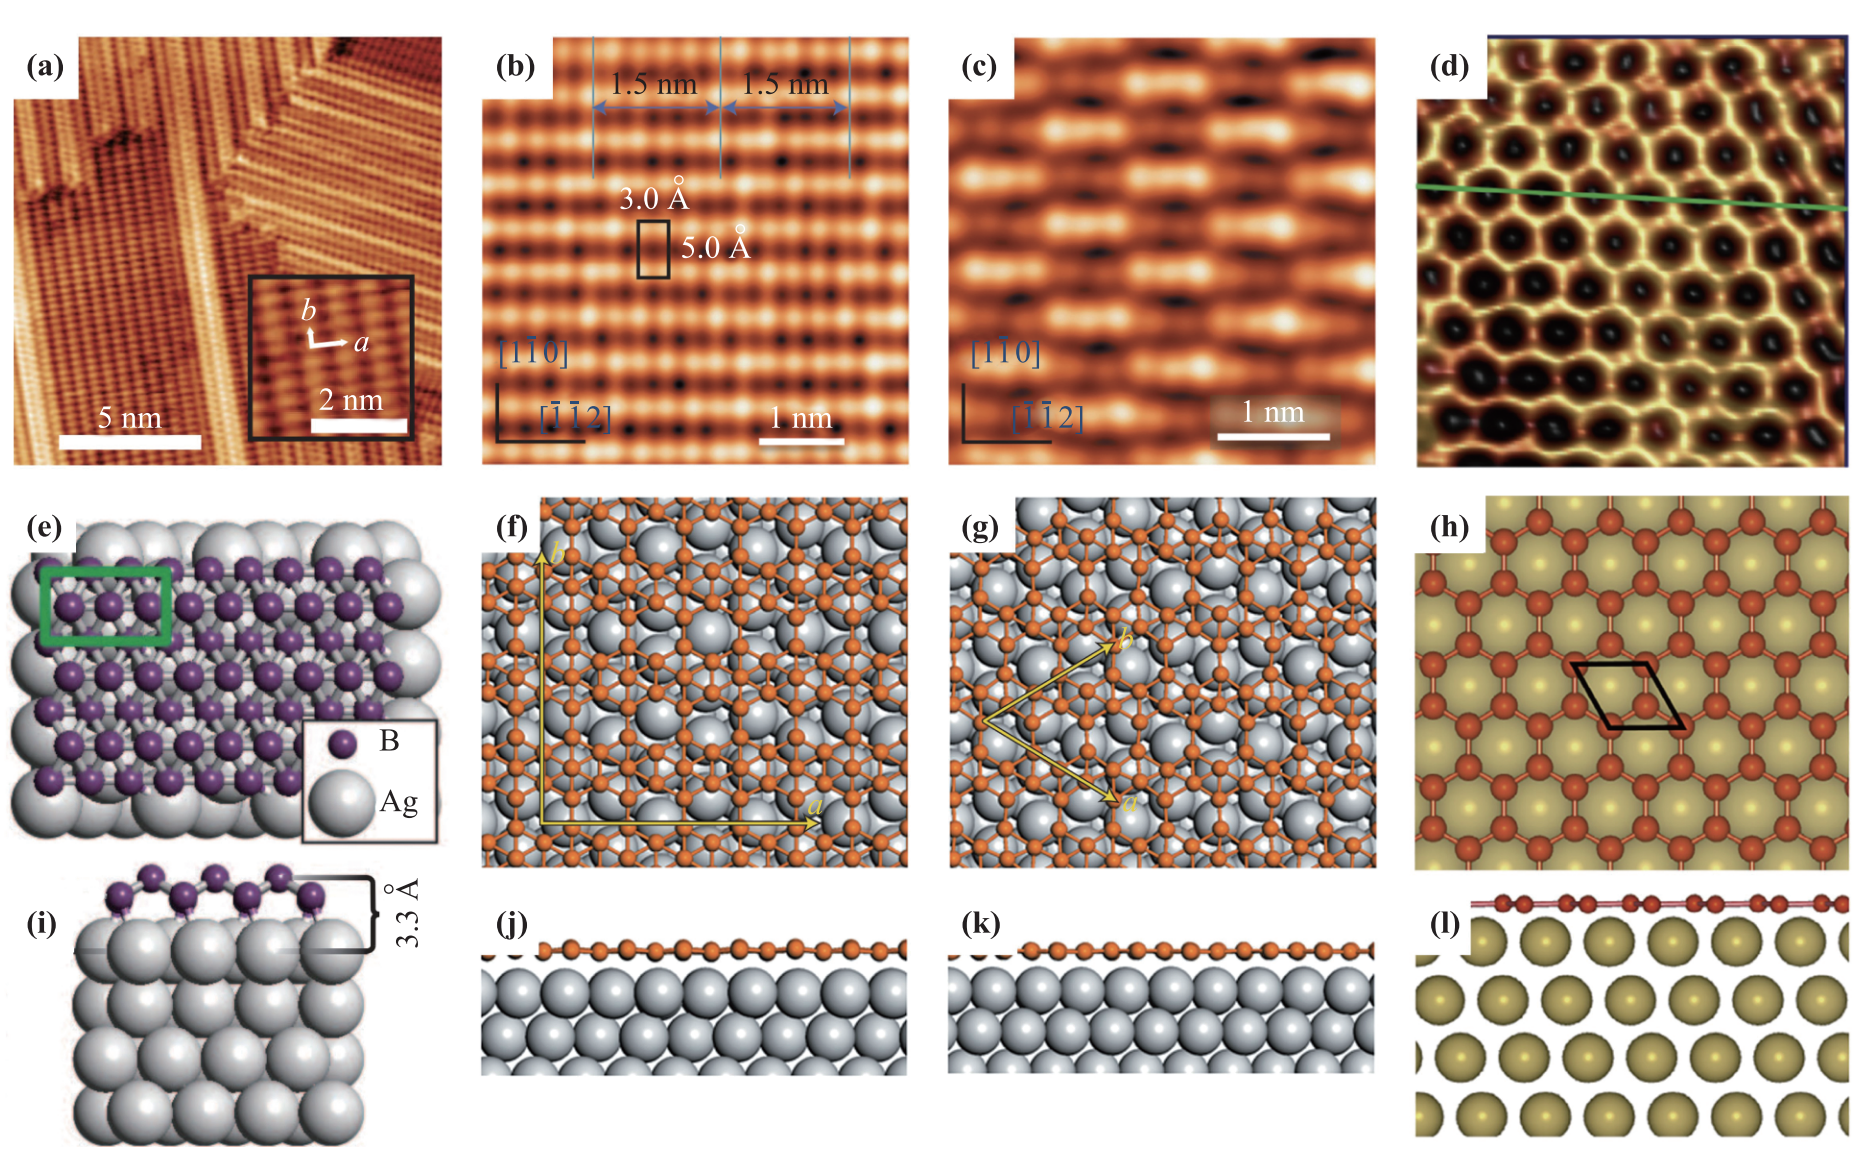
\includegraphics[width=1.0\textwidth]{figs/ch1_boron4phase.png}
  \centering
  \caption{硼在银/铝衬底上生长的2-$Pmmn$, $\beta_{12}$, $\chi_3$, 蜂窝相,(a-d)为STM电镜图,(e-h)为俯视图,(i-l)为侧视图,图片来源并整理自文献\cite{mannix2015synthesis,li2018experimental,feng2016experimental}}
  \label{fig:boron4phase}
\end{figure}

其它的二维硼的同素异形体都是由理论预测所报道的\cite{liu2018intermixing, liu2013probing, penev2012polymorphism, zhang2017elasticity, zhao2016superconductivity, yang2008ab, zhang2016polyphony, tsafack2016thermomechanical, zhang2016substrate, ma2016graphene}。
硼烯的稳定性与硼平面中空位的浓度有重要的联系,我们设平面三角网格中六角空位的比例为$x$,则$x$可能的取值必定在完全的三角网格和石墨烯形的六角格子的空位率之间。
如图\ref{fig:ch1_formation_boronphenes}所示,硼平面的形成能的空位率的变化呈现V型的关系,即从完全的三角格子向六角格子过渡,形成能先随着空位率的增加而降低(变得更稳定),在达到一定数值后又随着空位率的增加而升高(变得不稳定)。在空位率为$x=1/9$时\cite{penev2012polymorphism},可以得到对应的最为稳定的结构,同时在相近的空位率为$x=1/8$和$x=2/15$时,同样有很低的形成能,因此认为这些结构都有可能稳定地存在。
与其他二维材料如石墨烯、硅烯、锗烯、氮化硼以及黑磷所不同的是,硼烯的各种平面结构中在最稳定的结构附近,存在大量形成能相近的构型。

\begin{figure}[bt]
  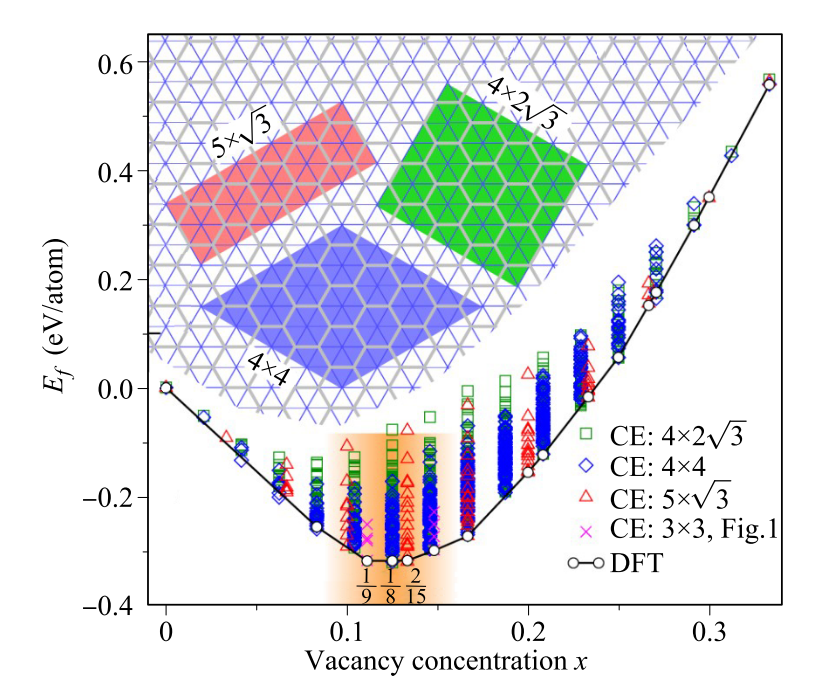
\includegraphics[width=1.0\textwidth]{figs/ch1_formation_boronphenes.png}
  \centering
  \caption{硼平面形成能$E_f$与硼平面空位率$x$的关系,图片来源文献\cite{penev2012polymorphism}}
  \label{fig:ch1_formation_boronphenes}
\end{figure}

除了和空位率相关,如前面所列举的,硼烯的稳定性还受到了衬底的影响。
Yakobson等提出\cite{zhang2015two},无衬底时的基态结构虽然形成能较低,但生长在衬底时却不一定是最稳定的。
如图\ref{fig:ch1_borophene_energy_spectra}所示,在银的111面衬底上,$\beta_{12}$相是最稳定的硼烯,其空位率为$x=1/6$.第二稳定和第三稳定的构型的空位率分别为$x=1/8$和$x=1/12$。
相应的形成能比最稳定的$\beta_{12}$构型要高出\SI{0.4}{\meV}和\SI{2.1}{\meV}。
在铜的111表面上能量最低的三种构型的空位率均为$x=1/6$,相比于能量最低的构型,次低和第三稳定的构型的形成能分别高出\SI{15.1}{\meV}的\SI{28.9}{\meV}\cite{zhang2015two}。这个结果表明,在铜的衬底上更有可能形成特定的统一的硼烯构型。

\begin{figure}[bt]
  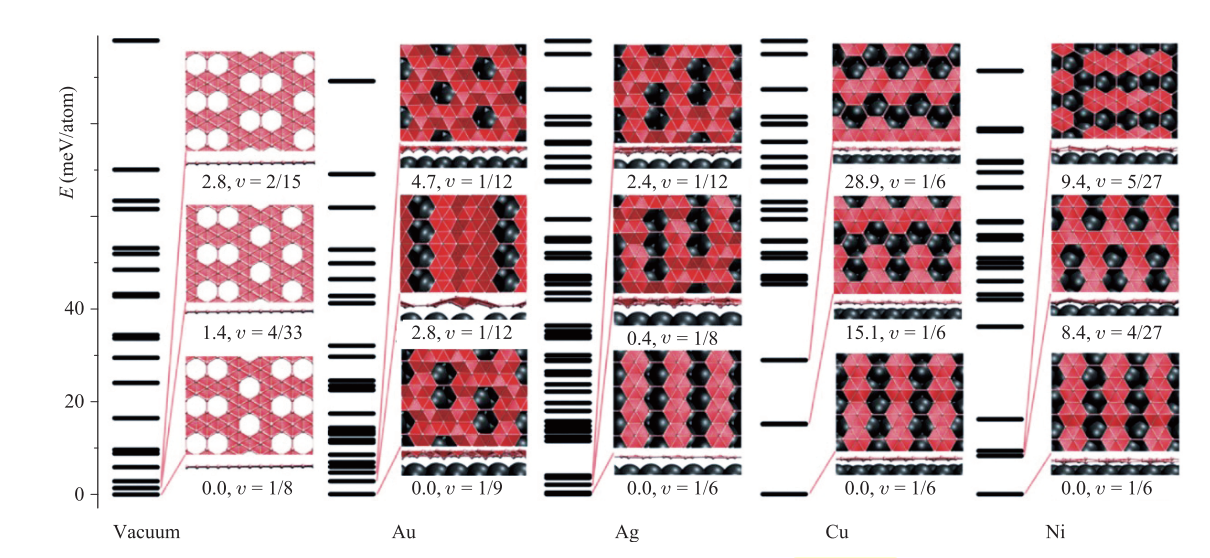
\includegraphics[width=1.0\textwidth]{figs/ch1_borophene_energy_spectra.png}
  \centering
  \caption{理论预测硼烯在金、银、铜、镍衬底上生长的能量谱,图片来源文献\cite{zhang2015two}}
  \label{fig:ch1_borophene_energy_spectra}
\end{figure}

除了空位率和衬底外,官能团修饰是调节硼烯物理和化学性质的另外一个有效手段。比如在其他二维材料如石墨烯、硅烯、锗烯中,
能够使用氢化的方法来增加半导体材料的带隙,或打开金属性材料的带隙将材料从金属变为半导体\cite{balog2010bandgap,bhattacharya2011strain,houssa2011electronic}。
同时官能团修饰后的材料在结构上也会发生明显的改变。石墨烯是完全平面的二维材料,但完全氢化后石墨烯结构呈现隆起状。
与石墨烯类似,硼烯也同样能通过官能团修饰的方法改性,通过氢化能改变硼平面结构的稳定性,比如对2-$Pmmn$相的硼烯进行氢化,声子谱在$\Gamma$点处的虚频消失,结构上更加稳定\cite{xu2016hydrogenated,wang2016high}。
氢化还会改变构型的电子结构\cite{xu2016hydrogenated},在对2-$Pmmn$相的硼烯氢化后,原结构对应电子结构中电子占据的反键部分的电子向氢原子发生转移,使得面内的成键轨道完全占据,反键轨道无占据,从而使结构更加稳定。而且,该氢化后的结构在布里渊区的$X-\Gamma$方向存在狄拉克锥的电子结构,狄拉克点处的电子速度为\SI{3.5e6}{\metre\per\second}\cite{xu2016hydrogenated}。另外,氢化后结构的力学性质也得到了改善,其面内两个方向的杨氏模量分别为\SI{172.24}{\N\per\meter}和\SI{110.59}{\N\per\meter}\cite{wang2016high}。

\subsection{二维硼材料的性质}
热传导性能是纳米器件使用性能和耐用性的重要指标。
有一系列的文献\cite{li2018stretch, mortazavi2018borophene, zhou2017superior, liu2017anisotropic, sun2016first, mortazavi2017anomalous}报道了二维硼材料有关这一性质的研究。
硼烯2-$Pmmn$相为各向异性,其热导也表现出极大的各向异性。室温时,2-$Pmmn$相沿锯齿状(zigzag)方向和沿椅式状(armchair)方向的热导分别为\SI{75.9}{\W\per\meter\per\kelvin}和\SI{147.0}{\W\per\meter\per\kelvin}。这两个方向的声子平均有效自由路程为\SI{16.7}{\nm}和\SI{21.4}{\nm}。
$\alpha$-硼平面具有各向同性,其热导为\SI{14.34}{\W\per\meter\per\kelvin}。硼烯中热导主要是由高频声子的振动模式所贡献的,这不同于在其他二维材料如石墨烯,硅烯,磷烯,这些材料的热传导性质主要是由低频的声子模式所决定的\cite{gu2015first,qin2015anisotropic}。

从实验上合成得到的单层硼平面结构,研究人员对其进行了系统的电子结构性质的研究。实验测试和理论计算的结果显示,得到的单层硼烯平面,原子起伏的2-$Pmmn$相,$\beta_{12}$相以及$\chi_3$相,都是金属\cite{shu2016unveiling},Yakobson等\cite{penev2016can}通过理论计算预测,这种金属单层硼平面应该具有超导电性质。同时,他们还进一步研究了该类金属二维材料其表面的光学性质\cite{huang2017two}。
Feng等\cite{feng2017dirac,feng2018discovery}人通过角分辨光电子能谱(ARPES)测量技术揭示(如图\ref{fig:ch1_boron_arpes}),在实验上对应的两种单层硼的相的电子结构能带中存在非平庸的狄拉克点,因此认为其有可能是二维拓扑材料。
之后,又有进一步的理论计算工作预言了在其他类型的单层硼平面的能带结构中,不但存在各项异性的狄拉克锥, 而且还存在有节线(node-line)特征的非平庸的色散关系\cite{zhang2017dirac}。
Du等\cite{jiao2016two}人的理论工作指出,六角晶格的单层硼平面,如果硼原子表面用氢原子修饰,也会实现各向异性的狄拉克点。

\begin{figure}[bt]
  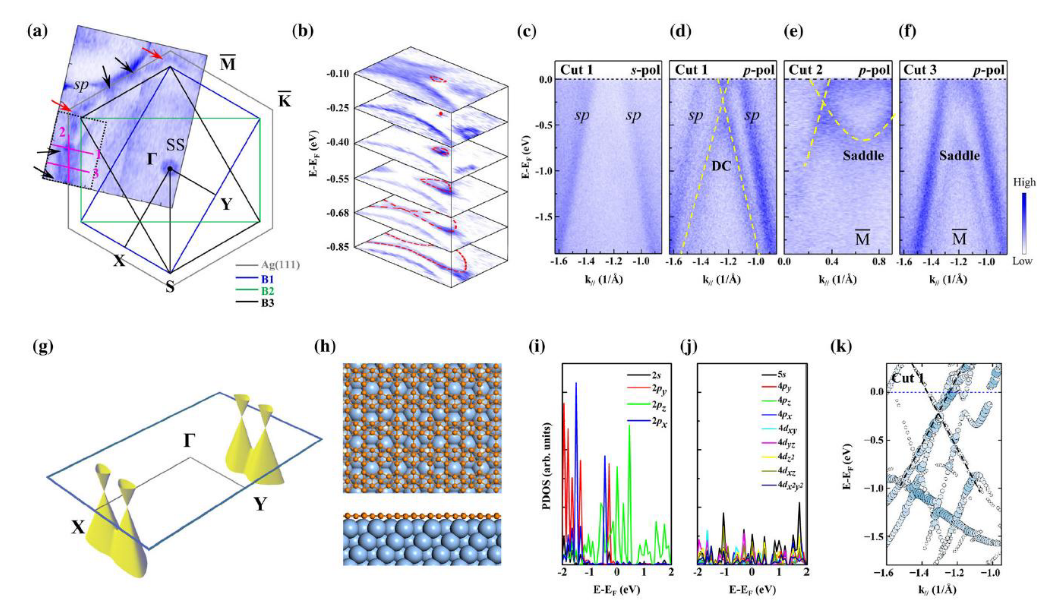
\includegraphics[width=1.0\textwidth]{figs/ch1_boron_arpes.png}
  \centering
  \caption{实验和理论计算的的$\beta_{12}$相在银111衬底上的电子能带结构,图片源于文献\cite{feng2017dirac}}
  \label{fig:ch1_boron_arpes}
\end{figure}

需要提及的是,理论预测不但辅助实验合成得到了二维单原子层硼平面,理论还预言了硼存在二维薄膜结构。然而,到目前为止并没有发现硼的层状体相材料的存在,目前已知所有的硼的体相构型都具有高配位的极其复杂的成键方式。如果使用全局构型搜索的方法,当不限制搜索时二维的材料的厚度时,有理论工作表明,多层的硼结构会比孤立单层硼平面更加稳定。
比如Zhou等\cite{zhou2014semimetallic}通过遗传算法理论预测了稳定的非单层的有狄拉克点的二维硼材料。
Du等\cite{ma2016graphene}的也发现了一种新型的具有双狄拉克色散的二维硼薄膜。
实验上,2015年南京航空航天大学科研团队在铜表面以硼和\ce{B2O3}为前驱体,通过加\ce{H2}还原的方式得到了二维硼薄膜\cite{tai2015synthesis},该硼薄膜被认为是从体相硼$\gamma_{28}$中切割出的单层结构。
他们理论计算表明,该硼薄膜材料是一种宽直接带隙的半导体材料,其相应的带隙值为\SI{2.07}{\eV},使其有可能被作为具有优秀光吸收性质的材料。
然而,后续又有其他的理论工作\cite{kou2016high}认为这种二维薄膜其实是金属,但如果在其表面通过氢原子进行修饰,可以容易的实现金属和半导体之间的调控。

单层硼平面的结构多样性非常丰富,然而,大多数理论计算和实验发现的单层硼平面都是金属\cite{zhang2017two},Yakobson等\cite{penev2012polymorphism,penev2016can}在多篇文献中认为,单层硼平面之所以呈现金属性,是因为其体系的费米能级一定会穿过由体系构型中平面结构面外垂直方向的$p_z$ 轨道所构成的能带。
但是体系本身的面内轨道($s$, $p_x$ 和 $p_y$轨道) 在费米能级处是可能存在带隙的。
所以普遍的观点认为,单层硼平面所有构型都不会表现出半导体性质。但我们课题组2017年的工作\cite{xu2017two}报道了理论预测的表现为半导体的几种硼平面构型,这大大的拓展了硼平面的性质。

对于石墨烯结构,可以将孤立的锂原子吸附在石墨烯表面。有理论计算指出\cite{profeta2012phonon},通过控制锂元素的覆盖度变化,可以得到不同的超导转变温度的二维超导体。随后,有另外的研究者\cite{wu2016lithium}将同样的思路拓展到单层硼平面的锂吸附性质上,通过结合集团展开来评估体系能量,他们预测了一系列随覆盖度变化而变化的\ce{Li/B} 超导体,其中所预测的\ce{Li2B7}构型的超导转变温度为\SI{6.2}{\kelvin}。 该研究说明了,通过控制覆盖度以及平面上的孤立原子的吸附位点,可制备出一系列超过液氦温度的传统BCS二维超导体。也正是这个研究引导了本论文关于钛硼单层超导性质的研究思路。

另外,硼平面的化学活性也有不少的相关研究,因为硼单层平面与金属锂具有强的吸附作用,被锂修饰的硼单层平面材料可以被设计用来作为高性能的储氢材料。
有理论\cite{li2015ultrahigh}预测稳定了具有$x=1/8$空位浓度的硼单层平面可能具有较理想的储氢性能。并且,实验上合成得到的硼平面结构也被用来实现锂离子电池的设计。
通过理论计算\cite{jiang2016borophene}发现,2-$Pmmn$相的起伏三角格子的二维硼结构沿其起伏形成的通道方向,其锂离子的扩散非常容易,对应的扩散势垒仅有\SI{2.6}{\meV}。
并且,实验上所合成得到的两种基态构型$\beta_{12}$相和$\chi_3$相本身就有较多的空位的分布,空位连接成链时其可以被看作是理想的离子扩散通道\cite{zhang2016borophene},但不理想的是,由于硼原子的缺电子性,这些空位对应的是较强的金属吸附,导致了锂原子沿这类链状空位路径扩散时的势垒约为\SI{0.6}{\eV}。
如下图\ref{fig:ch1_lina_borophene}所示,分别是$\beta_{12}$相和$\chi_3$相锂离子扩散和钠离子扩散的模拟路径。
相比于其他的二维材料,单层硼烯具有较大的吸附能。
理论计算表明\cite{ling2017nanosheet},在实验上单层$\beta_{12}$平面的六角空位处吸附孤立的金属原子铋,可以作为一个非常有效的单原子催化载体从而可以实现水分解,$\beta_{12}$平面还可作为绿色环境材料用于实现对温室气体\ce{CO2}的高效捕获\cite{tan2017borophene}。

\begin{figure}[bt]
  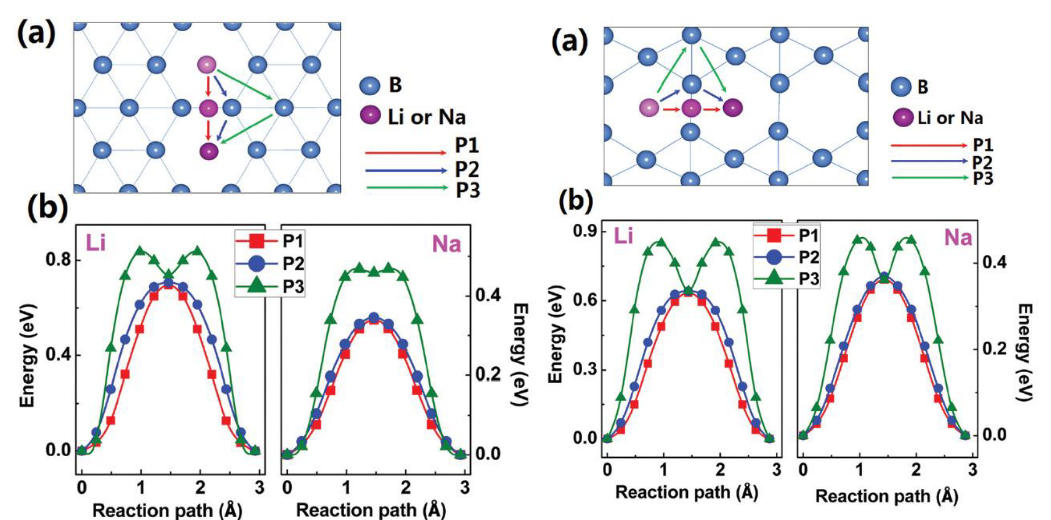
\includegraphics[width=1.0\textwidth]{figs/ch1_lina_borophene.png}
  \centering
  \caption{理论模拟的锂/钠离子在$\beta_{12}$和$\chi_3$表面的扩散路径,图片源于文献\cite{zhang2016borophene}}
  \label{fig:ch1_lina_borophene}
\end{figure}

\subsection{过渡金属硼平面及其理论计算研究进展}
研究原子团簇结构和性质之间的关系,对理解化学键本质以及设计性质可调控的纳米材料有重要的意义。
硼原子由于其缺电子性,较少的硼原子在形成团簇时倾向于形成平面团簇结构\cite{xu2017practical},这一特征和硼的体相结构及体相含硼化合物中的硼复杂网络结构形成鲜明对比。
硼的阴离子团簇最大可达到23个原子\cite{alexandrova2004molecular, alexandrova2004electronic, kiran2005planar, alexandrova2006all, sergeeva2008photoelectron, huang2010concentric, sergeeva2011all, piazza2012photoelectron, sergeeva2012b22, zhai2003hydrocarbon, zhai2003hepta},
在硼原子数量为16的硼阳离子团簇和硼原子数量为20的中性硼原子团簇中,均发现了结构从二维到三维的转变\cite{kiran2005planar, tai2012structure, oger2007boron}。
所有实验发现的硼平面团簇\cite{romanescu2013transition},都是由一圈通过二中心二电子(2c-2e)硼硼键所形成的硼环围绕一个中心原子,硼和中心原子通过$\sigma$键连接,整个平面团簇在水平方面形成一个大$\pi$键来稳定团簇。
我们可以注意到,在阴离子硼团簇中,中心原子通常和多个硼原子形成多中心键,一个典型的例子是\ce{B19^-}(\ce{B}@\ce{B5}@\ce{B13})\cite{huang2010concentric},其中就包含两种不同的离域$\pi$键。
这种离域表示了中心硼原子与中间层的\ce{B5}环,\ce{B5}环与最外层\ce{B13}环之间的相互作用。有趣的是,内层的\ce{B}@\ce{B5}结构可以在\ce{B13}环中自由旋转,这使其成为了分子器件的一个潜在候选。

当八个或九个硼原子成环时,可以在环的中央放入金属离子而形成稳定的团簇结构,这两种轮状团簇是有高对称性的轮状分子,其中硼元素组成的环符合$(4N+2)$休克尔规则,使得结构能够稳定存在\cite{zhai2003hepta,alexandrova2004molecular}。
已经被实验报道的有\ce{AlB7^-}($C_{7v}$)和\ce{AlB^-}($C_{8v}$)\cite{galeev2011valence},结构中的铝元素分别和\ce{B7}与\ce{B8}环通过离子相互作用结合,
金属-硼之间的成键并不离域。2013年Romanescu等通过激光蒸发喷射超快团簇束的方法得到了一系列以过渡金属为中心与硼环形成的轮状分子结构,\ce{Co}@\ce{B8^-}, \ce{Ru}@\ce{B9^-}, \ce{Rh}@\ce{B9^-},\ce{Ir}@\ce{B9^-}, \ce{Nb}@\ce{B9^-}以及 \ce{Ta}@\ce{B9^-} \cite{romanescu2011aromatic,galeev2011valence,li2012transition},
这些实验发现的结构(如图\ref{fig:ch1_boron_wheel01}和图\ref{fig:ch1_boron_wheel02}所示)也同样被理论证实是该化学配比下能量最低的平面团簇结构。

\begin{figure}[bt]
  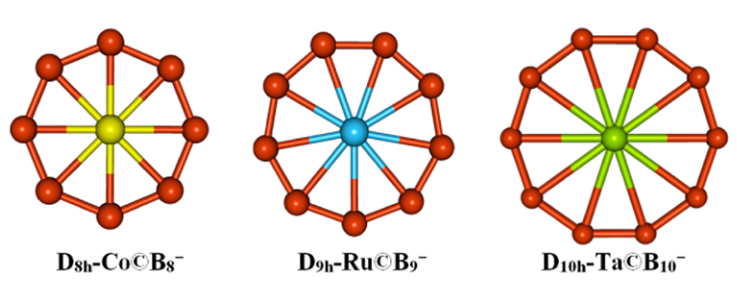
\includegraphics[width=0.86\textwidth]{figs/ch1_boron_wheel01.png}
  \centering
  \caption{轮状结构的\ce{Co}@\ce{B8^-},\ce{Ru}@\ce{B9^-}和\ce{Ta}@\ce{B10^-},图片源于文献\cite{romanescu2013transition}}
  \label{fig:ch1_boron_wheel01}
\end{figure}

\begin{figure}
  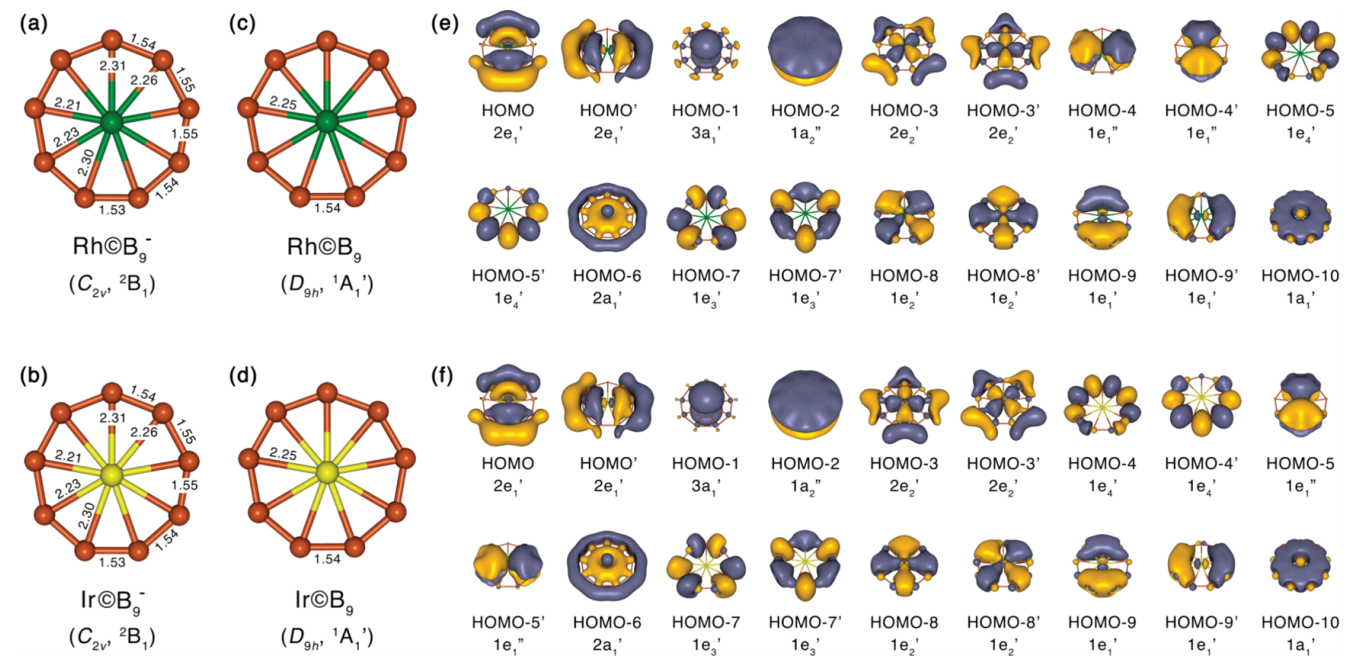
\includegraphics[width=1.0\textwidth]{figs/ch1_boron_wheel02.png}
  \centering
  \caption{优化后的金属硼团簇轮状结构(a)\ce{Rh}@\ce{B9^-},(b)\ce{Ir}@\ce{B9^-},(c)\ce{Rh}@\ce{B9}和(d)\ce{Ir}@\ce{B9}以及理论计算的价层电子分子轨道,图片源于文献\cite{li2012transition}}
  \label{fig:ch1_boron_wheel02}
\end{figure}

\begin{figure}[bt]
  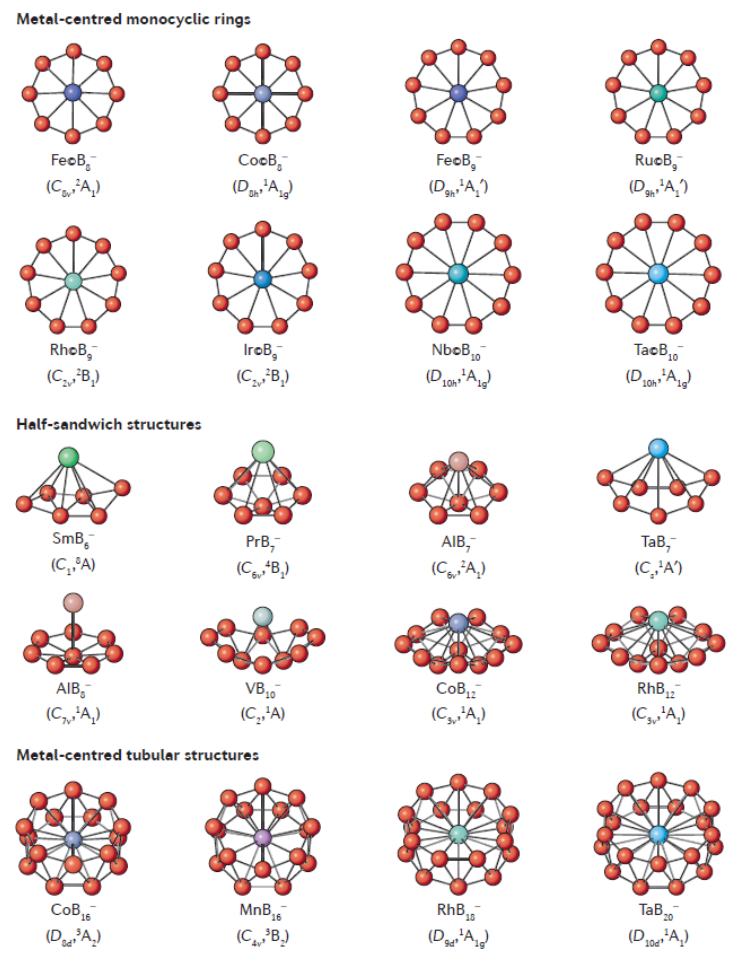
\includegraphics[width=0.96\textwidth]{figs/ch1_boron_metal_cluster.png}
  \centering
  \caption{金属原子与硼团簇结合后形成的稳定纳米结构。本图源于文献\cite{li2017planar}}
  \label{fig:ch1_boron_metal_cluster}
\end{figure}

结合过渡金属与硼形成的轮状结构的稳定性和硼平面的多样性,我们可以将过渡金属硼平面看作是由过渡金属嵌入硼平面中所形成的稳定构型。理论预测报道了许多这样的材料并报道了它们相关的物理化学性质。

Qu等\cite{qu2017two}使用粒子群算法对钛硼比例为$1:4$的结构进行了搜索,找到了全平的二维单层钛硼结构,如图\ref{fig:ch1_tib4}所示,其中钛原子被八个硼原子环绕形成八配位的钛硼轮状结构,八个硼原子到钛原子的距离均相等。他们计算了该结构的动力学性质,认为其十分稳定因而可能够被实验所合成。同时他们认为该结构的稳定性源于钛和硼形成的八配位的稳定轮状团簇,因为钛向硼提供了电子弥补了硼的缺电性使硼原子之间形成了$sp^2$杂化轨道构成的稳定网络。受该结构启发,他们还对该钛硼结构进行了其他金属原子的替换,将钛替换为钒,镉,锰,钨元素形成平面或准平面结构并讨论了这些结构的稳定性。

\begin{figure}[bt]
  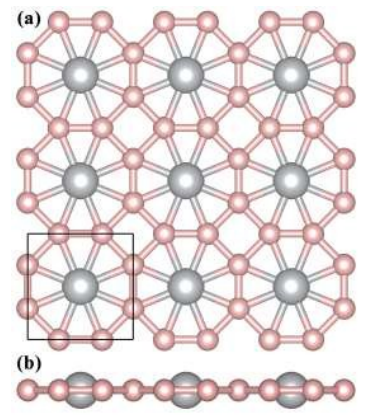
\includegraphics[width=0.42\textwidth]{figs/ch1_tib4.png}
  \centering
  \caption{\ce{TiB4}单层平面的俯视图(a)和侧视图(b),图片源于文献\cite{qu2017two}}
  \label{fig:ch1_tib4}
\end{figure}

Bo等\cite{bo2019tetragonal}通过第一性原理结合粒子群算法,发现并研究了两种\ce{Mo2B2}单层的稳定性,电子结构,晶格动力学性质以及其在电池材料中作为阴极材料时的性质。声子谱和电子结构的信息展示了正方和三方晶系\ce{Mo2B2}结构(如图\ref{fig:ch1_mo2b2})的高电导性质以及高的稳定性。这两个结构对锂原子和钠原子的吸附能在电池的工作范围内都非常大,确保了其工作效率。其中正方晶系\ce{Mo2B2}的锂离子和钠离子容量均为约\SI{251}{\mA\hour\per\g}, 三方晶系\ce{Mo2B2}的锂离子和钠离子容量分别为约\SI{251}{\mA\hour\per\g}和\SI{188}{\mA\hour\per\g}。
三方晶系的\ce{Mo2B2}对锂离子和钠离子的扩散势垒分别为\SI{0.023}{\eV}和\SI{0.013}{\eV},四方晶系\ce{Mo2B2}对锂钠离子的扩散势垒分别为\SI{0.029}{\eV}和\SI{0.010}{\eV},较低的扩散势垒说明他们有很好的充放电效率。
相同研究组的研究人员还在另一工作中对六方晶系\ce{Ti2B2}\cite{bo2018hexagonal}进行了锂离子和钠离子电池性质的研究,该材料的锂钠离子的容量分别为\SI{456}{\mA\hour\per\g}和\SI{1027}{\mA\hour\per\g}。
值得一提的是该材料对锂离子和钠离子的扩散势垒非常低分别仅为\SI{0.017}{\eV}和\SI{0.008}{\eV},因此推断其具有非常优良的充放电性质。

\begin{figure}[bt]
  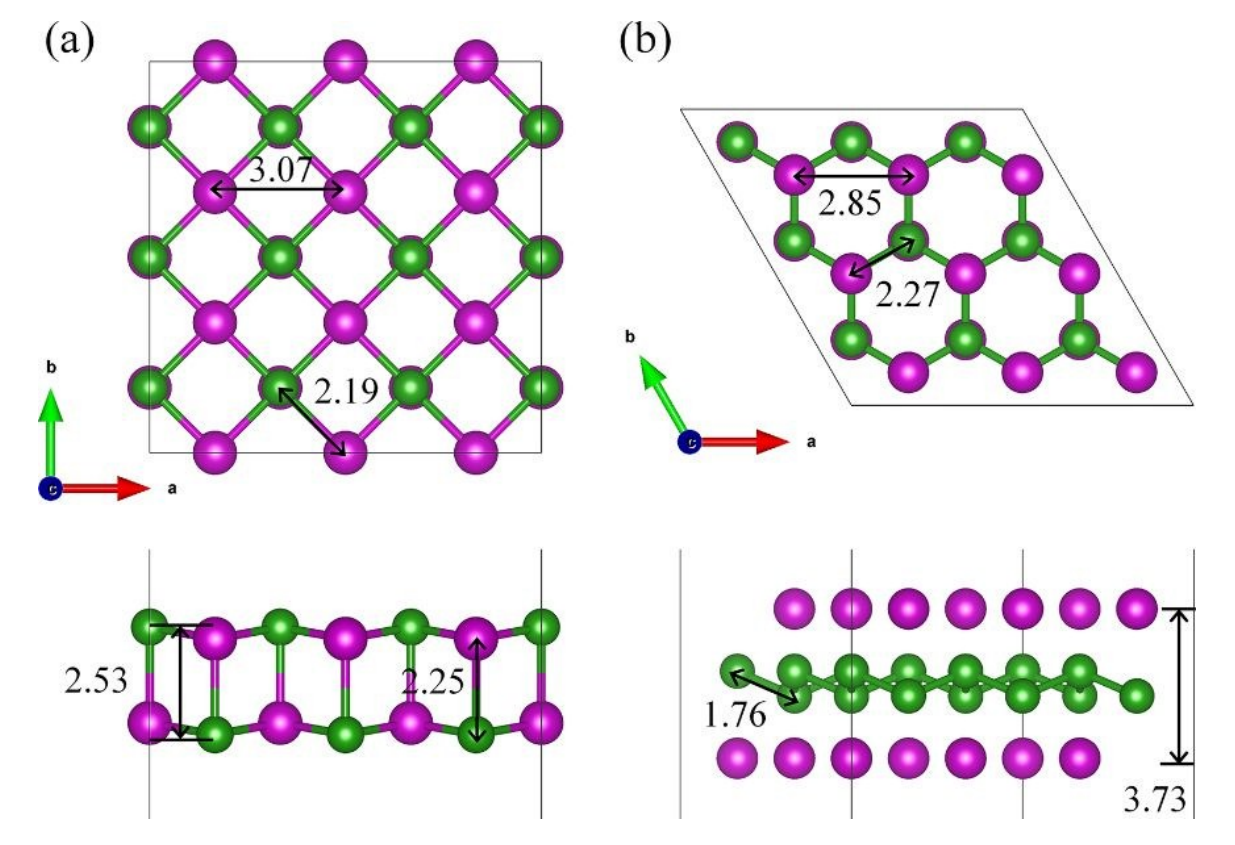
\includegraphics[width=0.86\textwidth]{figs/ch1_mo2b2.png}
  \centering
  \caption{正方和三方晶系Mo2B2结构的俯视图和侧视图,图片源于文献\cite{bo2019tetragonal}}
  \label{fig:ch1_mo2b2}
\end{figure}

Tang等\cite{tang2019cob}使用粒子群算法预测了钴原子和硼原子形成的单层平面化合物\ce{CoB6}(结构如图\ref{fig:ch1_cob6}所示),并研究了该材料的磁学和电学性质。动力学计算显示该材料有很好的稳定性,同时他们认为该平面\ce{CoB6}是稳定的二维铁磁材料,而且其磁矩和磁稳定性能够通过对材料施加应力来提高。他们还探讨了对该材料可能的合成方法,认为可以通过在已经被实验所报道的$\delta_4$相硼单层平面上,通过吸附钴原子或直接通过化学生长得到该结构。

\begin{figure}[bt]
  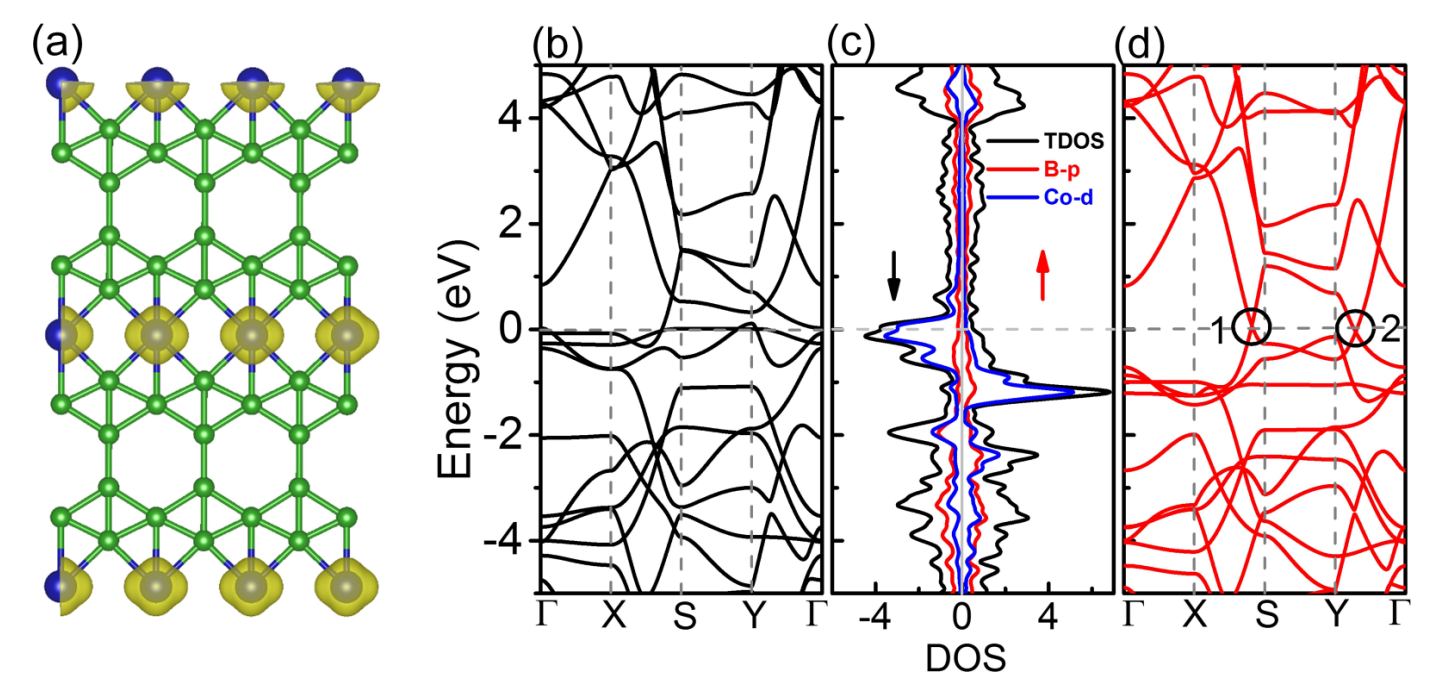
\includegraphics[width=1.0\textwidth]{figs/ch1_cob6.png}
  \centering
  \caption{(a)单层\ce{CoB6}自旋未配对电荷密度分布(b)自旋向下部分的能带(c)态密度(d)自旋向上部分的能带,图片来源文献\cite{tang2019cob}}
  \label{fig:ch1_cob6}
\end{figure}

Wang等\cite{wang2017semimetallic}通过使用第一性原理计算结合全局搜索算法,发现了一系列\ce{TiB_x}($2\leq x\leq 16$)结构,由钛和硼原子在二维平面排列组成。这些结构因为被钛原子到硼原子的电子转移而更好的稳定。因此,拥有比目前提出的二维硼平面的更好的稳定性。特别是,他们发现了\ce{TiB12}具有足够低的能量,使其可在\ce{TiB2}和二维$\alpha$-硼平面构成的混合物中能够稳定存在。同时,\ce{TiB12}具有带隙为\SI{0.02}{\eV}的准狄拉克点。有趣的是,他们还计算出这种二维\ce{TiB12}材料的功函数和电导率可以通过施加轴向应变进行调节。该二维\ce{TiB12}的合成和新的电子特性使其成为一种有前途的纳米电子应用的新型二维材料。这篇文献中所报道的单层的钛硼平面恰好为本论文的工作提供了充足的参考,本论文的工作在文献所报道的单层钛硼结构的基础上,还得到了一些能量更低的单层钛硼构型并研究了它们的超导性质。


\section{硼化物的超导性质研究进展}

原子质量小的元素所构成的金属材料会展现新颖的电子结构性质,硼作为原子质量较轻的一个元素,单质硼或硼化合物往往会有相对较高的超导温度。
2001年Eremets等\cite{eremets2001superconductivity}通过金刚石对顶针在超高压160GP下将硼从非金属相转变为金属相,并表现出超导性质,当压力从\SI{175}{\GPa}升高到\SI{250}{\GPa}时,其超导温度从\SI{6}{\kelvin}提升到了\SI{11.2}{\kelvin},即每\si{\GPa}压力增加可提高临界温度\SI{0.05}{\kelvin},理论计算表明该高压材料的超导为BCS机制的超导,对临界温度的理论计算结果与实验测量结果相符合。
同年,Nagamatsu等\cite{nagamatsu2001superconductivity}报道了具有最高临界温度的非铜氧型的超导体\ce{MgB2}\cite{buzea2001review},其常压下超导温度为39K。
与\ce{MgB2}由相同结构的化合物\ce{AlB2}同样表现出超导性能,但常压下的超导温度为较小,有趣的是能够通过多种手段调节使其超导温度提升。
同类型结构,不同金属元素的\ce{XB2}型化物也同样存在超导性,如\ce{ZrB2},\ce{HfB2}\cite{barbero2017doping},\ce{NbB_{2+x}}\cite{mudgel2008superconductivity}以及\ce{TaB_{2+x}}\cite{singh2001superconductivity}。
这种材料在结构上表现为硼原子以六角格子网络连接,金属原子以插层形式位于硼网络层之间,如图\ref{fig:ch1_mgb2}。这种层状嵌套的结构特征启发研究者们,可能会存在二维的硼或硼化物和超导材料。

\begin{figure}[bt]
  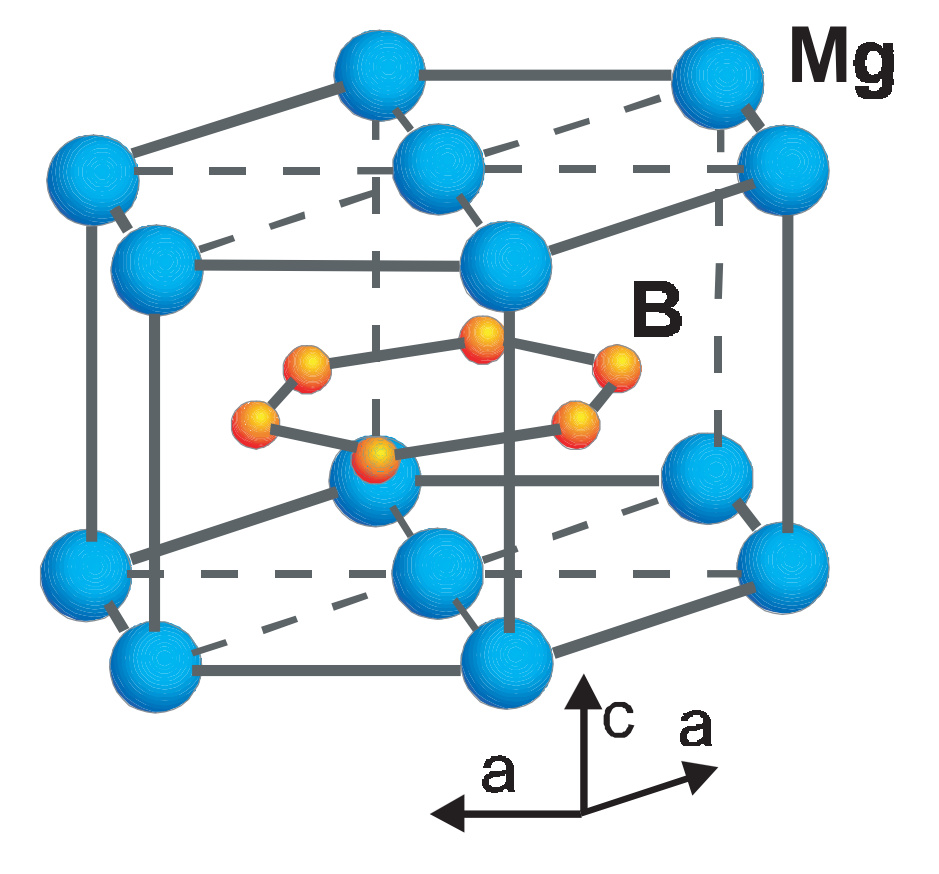
\includegraphics[width=0.60\textwidth]{figs/ch1_mgb2.png}
  \centering
  \caption{\ce{MgB2}(其他元素的超导相由类似结构)的结构图,其中\ce{B}元素形成石墨烯类似的六角格子网络,\ce{Mg}原子嵌入在硼元素组成的六角格子网格堆叠的层之间。}
  \label{fig:ch1_mgb2}
\end{figure}

二维材料的超导性质在纳米超导量子器件\cite{pribiag2015edge}和纳米超导晶体管\cite{el2013superconductivity}中都有重要的潜在应用价值。通过在石墨烯上沉积金属原子的方式,能够使其出现超导性。
2007年首次报道了通过等离子方式在石墨烯上覆盖金属而诱发超导\cite{uchoa2007superconducting},后续的理论计算表明其超导温度为\ce{LiC6}单层8.1K\cite{gholami2018superconducting},和\ce{CaC6}单层1.4K\cite{yang2014superconducting},通过增加石墨烯层数,超导临界温度会发生改变。
与石墨烯类似,硼二维材料也能表现出超导性质。
2017年,Gao等\cite{gao2017prediction}对实验上能够在银111面上生长的$\beta_{12}$和$\chi_3$两种硼平面进行了超导性质的计算,预测其临界超导温度分别为\SI{18.7}{\kelvin}和\SI{24.7}{\kelvin}。
根据2012年Profeta等\cite{profeta2012phonon}报道的在石墨烯上吸附锂元素能够得到有超导性质的层状结构,2016年Wu等\cite{wu2016lithium}对锂在硼平面上沉积的结构进行了超导性质的计算,发现了一系列可能稳定存在的锂硼层状超导结构。2019年Yan等\cite{yan2019prediction}预测了两种稳定的\ce{Mo2B2}结构并计算了它们的超导临界温度为\SI{3.9}{\kelvin}和\SI{0.2}{\kelvin},并发现其电声耦合主要是由于钼原子的低频振动所导致的。

\section{结构搜索与高通量方法在硼材料研究中的应用}

原子在空间中能够以各种各样的形式堆积,从而形成各种类型的凝聚态物质,物质结构,是深入理解物质物理化学性质的非常重要的信息之一。《自然》杂志主编John Maddox曾在《自然》上发表评论称,“依据且仅依据物质的化学组分来确定物质的结构,是物理学的一个重要挑战”。通过计算材料学,从理论上预测和设计具有新颖或优良性质的材料具有极其重要的意义。原因是,理论计算的成本相比于实验较低,且不乏重要的前瞻性,对实验研究中以试错为主要探索方式的方法过程具有很强的指导意义。另外,理论计算的探索和研究,能够帮助研究人员从本质来理解材料结构的其物质性质之间的内在联系,并提供通过结构改变物质性质的关键信息,指导新材料的设计和发现。这样的研究方法对各种物质性质的研究都有着重要的价值。

在过去,科学家只能对已有的材料进行研究,通过实验表征其各种物质性质。因此,对物质性质的改性也往往只能限制在已有的物质结构的基础上,这大大限制了对材料性质的探索。近年来,科学家发展了一些新的结构搜索程序比如基于粒子群优化机制的CALYPSO程序\cite{wang2012calypso}、基于遗传算法的USPEX程序\cite{glass2006uspex}。
仅需要材料元素种类和配比,不需要任何结构信息,就可以产生大量可能的结构, 然后对这些结构进行优化和能量比较, 得出能量较低的结构,可再进一步研究这些结构的各种性质。结构搜索程序的日趋成熟加上服务器计算能力的提高, 极大地推进了探索新型材料的进程。即使对于实验上已经存在的材料,研究者采用结构搜索程序也能对其可能在其他极端条件下存在的未知构型进行进一步的探索和尝试。

硼原子能够组成许多原子数不同尺寸各异的硼团簇,且这些硼团簇具有新奇的电子结构特征。
通过CALYPSO,Wang等\cite{lv2014b38}2014年报道了38个硼原子组成的硼团簇,该团簇有很好的稳定性,
较大的能带和高的芳香性。如果再引入其他原子,那么硼还能够形成更加丰富的多配位团簇构型\cite{lv2015stabilization},
如图\ref{fig:ch1_boron_cluster01}和图\ref{fig:ch1_boron_cluster02}所示,通过结构搜索算法研究人员找到了一系列金属-硼团簇。
\ce{Li2B24}\cite{dong2019li}为管状结构,具有多重芳香性,能够用于生长硼纳米管。碱土金属镁能够和硼形成具有高稳定性的鼓状结构\ce{MgB18}团簇\cite{tian2019exhaustive}。铍元素能够和硼形成形似的团簇如具有二次旋转轴的\ce{BeB16^-}团簇\cite{kang2019probing}。与硼同处于第13族的铝与硼有相同的价电子结构,铝元素对硼团簇结构的影响较小,但能够增加其稳定性,铝硼能够形成环状平面结构\ce{AlB18^-}\cite{jin2019structural},有很大的带隙和较高的芳香性。
一通过结构搜索方法Tian等\cite{tian2019cluster}还找到了一大类过渡金属-硼团簇,这给周期性体系过渡金属硼的构建提供了丰富的构型资源。

在二维硼平面的结构搜索中,Wu等\cite{wu2012two},使用第一性原理粒子群算法,预测了两种稳定的单层硼平面$\alpha_1$平面和$\beta_1$平面,他们的能量均比原先报道的由Tang和Yang等\cite{tang2007novel,yang2008ab}分别报道的$\alpha$硼平面以及由Yakobson等\cite{penev2012polymorphism}报道发现的$\beta$硼平面的结合能更低。
利用全局结构搜索软件,Qu等\cite{qu2017two}预测发现稳定的\ce{TiB4}结构。
Zhang等\cite{zhang2017dirac}报道发现了能带结构中具有狄拉克锥的\ce{FeB6}结构。

\begin{figure}[bt]
  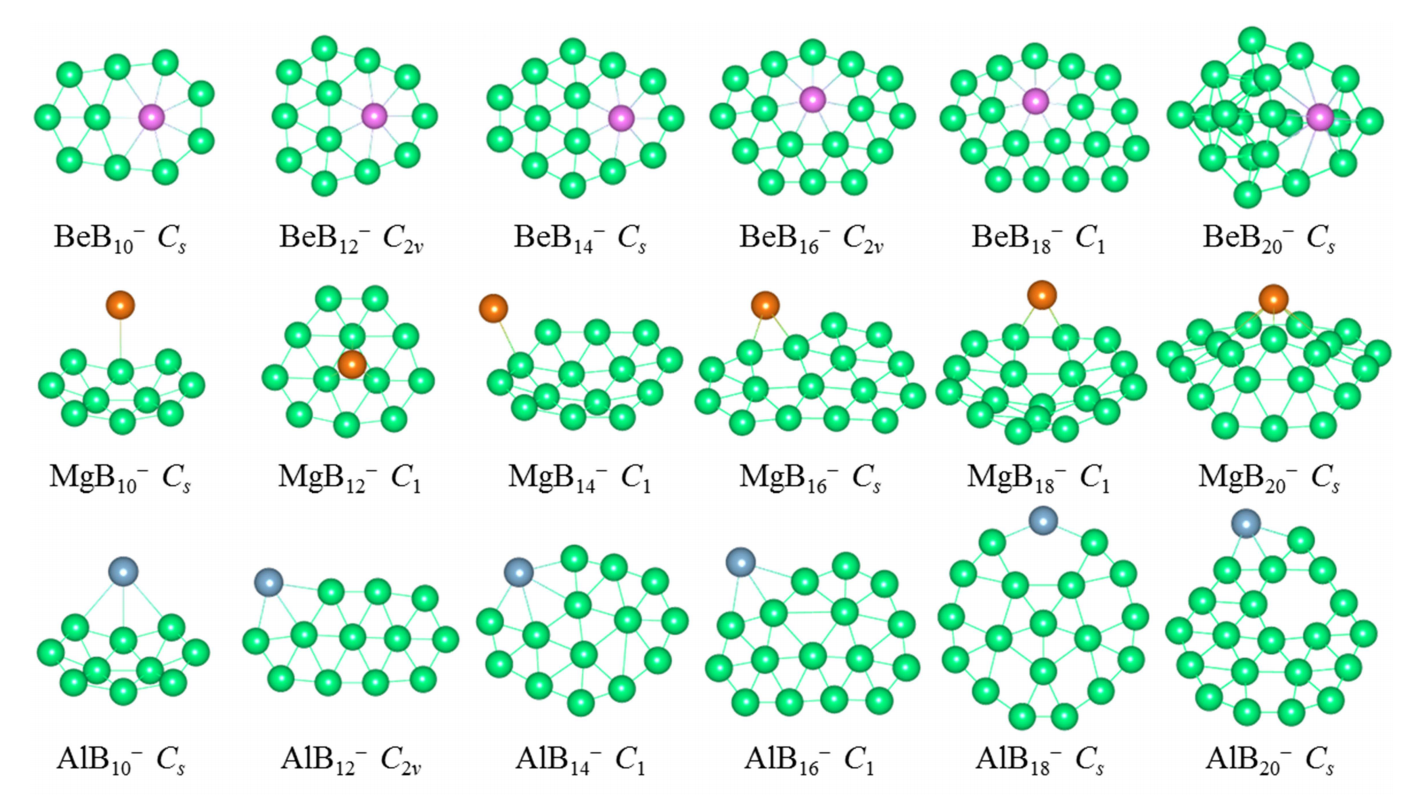
\includegraphics[width=0.96\textwidth]{figs/ch1_boron_cluster01.png}
  \centering
  \caption{金属原子Be,Mg,Al与硼团簇结合后形成的稳定纳米结构。本图源于文献\cite{tian2019cluster}}
  \label{fig:ch1_boron_cluster01}
\end{figure}

\begin{figure}[bt]
  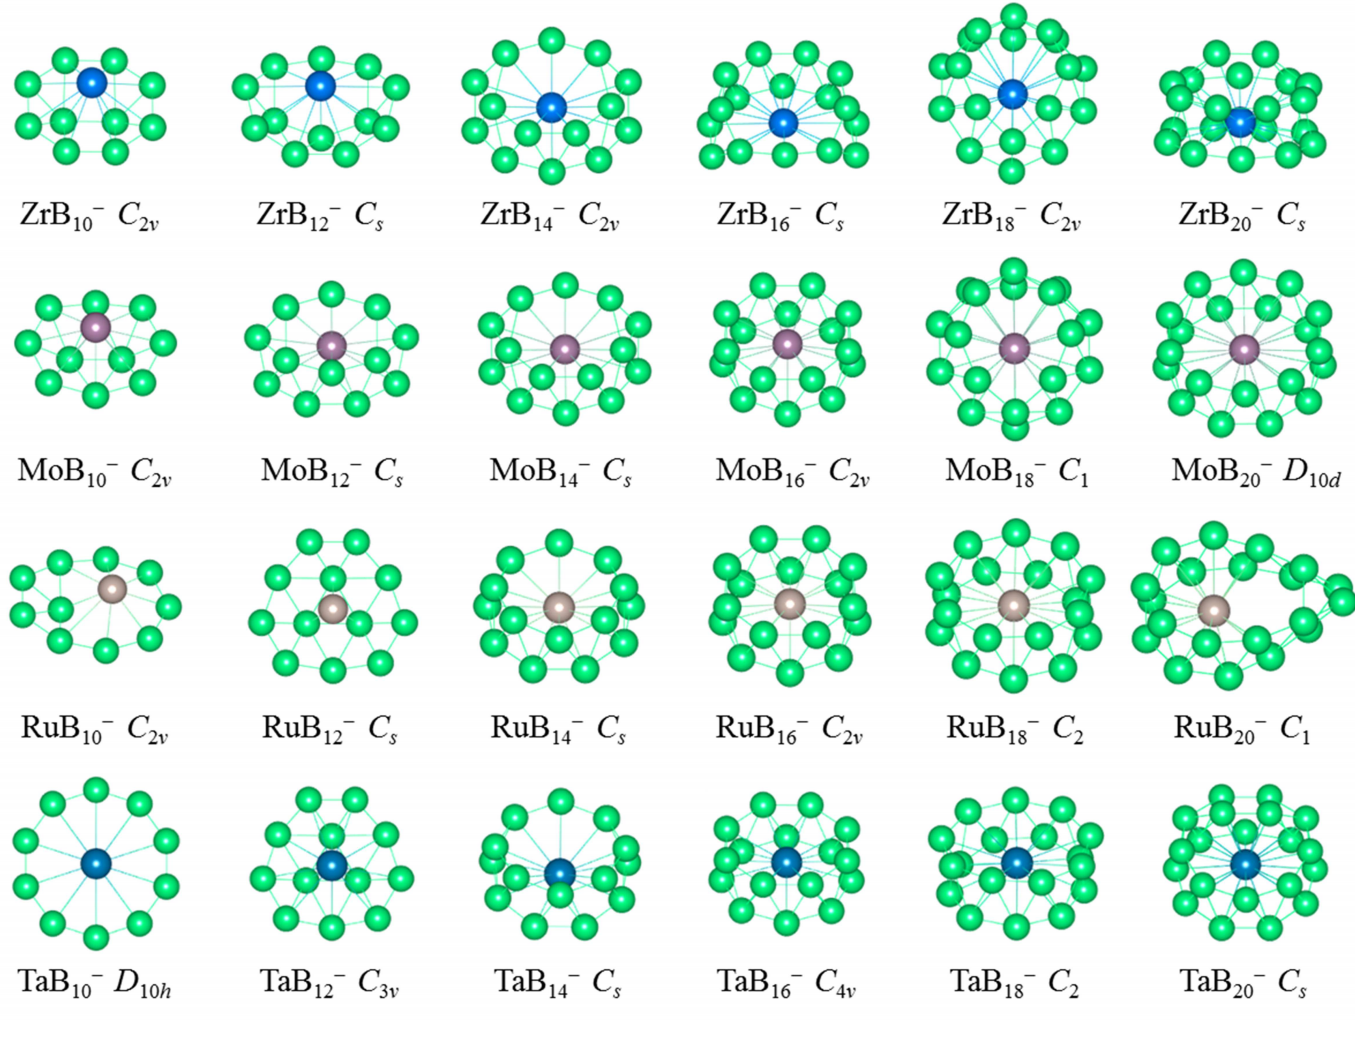
\includegraphics[width=0.96\textwidth]{figs/ch1_boron_cluster02.png}
  \centering
  \caption{金属原子Zr, Mo, Ru, Ta与硼团簇结合后形成的稳定纳米结构。本图源于文献\cite{tian2019cluster}}
  \label{fig:ch1_boron_cluster02}
\end{figure}

高通量计算材料学的方法,是与结构搜索对应的一种结合理论计算和数据分析技术来指导材料制备和研究的方法。
实验科学家通过规律和经验将某种材料合成并生长到能够完整测量其性质的规模往往是一个并不简单,及其耗费时间的过程。
因此材料从发现到实际的工业应用是非常缓慢的。这个过程中的许多步骤往往有极大的可重复性,并且不同材料间很可能因为细微的变量变化而出现性质上的巨大差别。
实验科学家有必要全面的考察各个变量所可能导致的结果差异。而这个过程中,就存在变量以外的如人工的重复。
信息化工业化的今天,将人的精力耗费在不断机械重复特定流程的工作中并不是一个理想的科学模式。
那么,高通量计算材料学就是这样一种方法,将重复的工作交由机械和计算机来完成,以解放科学家的时间和双手,使得科学家能够着眼于问题本身的探索。
今天,高通量实验科学尤其是高通量计算材料学已经发展出一套成熟和完整的方法\cite{curtarolo2003predicting, ceder1998identification, johannesson2002combined, curtarolo2005accuracy, xiang1995combinatorial, koinuma2004combinatorial, takeuchi2003identification}。

高通量计算材料学是使用高通量的方法结合计算材料学进行材料的设计。它是计算材料学与基于数据库构建,数据挖掘的计算机技术的结合。
通过对已有和理论预测的材料进行热力学、电子结构等性质的计算,之后将所得信息储存进入数据库,通过数据挖掘技术来筛选预测可能具备某种特别优秀性质的材料。
这个流程准确地符合了广义上的经验主义的科学方法论,即通过归纳来描述某类共有的科学现象并总结为规律,并且该规律还需要拥有演绎推广和预测未知的能力。我们希望将这个方法发展并应用到具有极大结构多样性的含硼化合物的结构与性质的研究中。

可以看到,硼元素因其独特的缺电子特性,在结构多样性上非常丰富,但同样可以看到,由硼所形成的结构都是由硼元素以密堆的方式形成网络,但由于其缺电子性,网络中需要空位或者其他元素原子作为电子给体来平衡电荷分布。根据以上特征,可以有选择的给出可能稳定的初始结构,使得所需要计算的结构数量大大降低而不再依赖于全局搜索算法。利用这样的方法,我们课题组对硼平面团簇结构进行了高通量结构搜索,对数千个候选结构进行能量的考察,不但能够全数找到已经被实验发现的平面团簇,还预测了稳定的\ce{B76}团簇\cite{xu2017practical}。通过对硼平面使用类似的方法,找到了具有半导体性质的硼平面结构\cite{xu2017two},这是首次发现报道的具有半导体性质的硼平面构型,这些构型的发现丰富了硼平面的性质,增加了硼平面应用上的潜质。在此基础上,我们在本论文的相关工作中将研究对象进一步扩充到了过渡金属和硼形成的二维材料中。通过结合新的高通量方法和工具,我们发现了一系列新的过渡金属-硼二维化合物,并研究了它们的性质。

\section{论文的研究意义和主要内容}
二维硼材料结构和性质上的多样性非常丰富,实验上研究人员已经能够生长出一定尺寸的单层硼材料,理论预测二维硼材料以及硼与其他元素所形成的二维化合物会表现出许许多多丰富的物理化学性质,尤其是当硼和过渡金属原子形成的二维化合物时,理论计算预测了很多新奇的性质,使二维硼化合物不但有应用上的潜力,同时也是很好的新物理现象的研究对象。
但硼在结构上丰富的多样性,一方面是其丰富的性质多样性的来源,但另一方面这也使得其合成和稳定结构的确定变得困难。如何发现和理论预测满足特定结构特定性质的二维硼材料,是本文研究的出发点。如果能从理论上预测具有优秀物理化学性质的二维硼材料,并对预测的材料的结构稳定性、结构特征、材料性质进行深入的研究,则能够指导和加快实验上对此类材料的发现和应用,从而大大减少材料科学中实验的人工成本和材料成本。

针对二维硼材料结构上的共性,我们使用加入结构相关的先验知识进行有偏向性的筛选和搜索(biased-screening)。
结果显示对我们关注的硼化物材料,这种方法的效果会优于使用全局搜索算法的无偏向性的结构搜索(unbiased-screening)。
通过加入硼二维材料中硼原子之间倾向于保持包含空位的硼平面三角网格的结构,我们使用结构查重软件优先构建了尽可能均匀分布于势能面空间中目标结构能量局域极小值点附近的初始构型。
再对所有生成的结构进行第一性原理计算以获得准确的能量和性质。
通过使用这个方法,我们研究了钛硼单层的稳定构型,不但发现了各个不同配比下已经报道过的几个钛硼单层材料,还发现了能量更低且具有优秀超导性质的\ce{TiB7}单层构型。
需要强调的是,通过加入先验的结构信息,我们所生成和计算的结构总数相比全局搜索算法所涉及的结构数量大大减少,该方法还更容易进行计算的管理,并且还获得了更好的结果。
因此,我们认为对于特定材料,如果其结构随上拥有固定特征,可以考虑使用该方法首先生成合理构型,来快速的筛选符合指定目标的结构。

本论文正文结构如下:
\begin{romanenum}
  \item 首先在第二章中介绍在论文相关的研究中所用到的理论方法,包括计算材料电子结构的密度泛函理论(DFT)和用于计算电声子互相作用的密度泛函微扰理论(DFPT),以及通过第一性原理计算超导性质作用到的理论方法。
  \item 第三章将重点阐述高通量材料计算的发展并引申出自动化工作流和数据库技术在高通量计算材料学中的重要性,最后集中描述AiiDA这一本论文研究中所用到的工作流工具的设计细节和使用方法。
  \item 第四章描述如何对固定晶格的材料生成不重复的晶格构型所涉及的算法和软件实现。
  \item 最后一章,则描述对钛硼构成的单层材料,利用第四章描述的工具进行不重复初始构型的生成,结构优化后得到局域稳定的构型,通过对结构的能量分析筛选可能稳定存在的构型并对其进行超导性质的研究。由于生成结构的数量非常巨大,在研究中我们使用了AiiDA作为高通量工具来自动化管理和生成计算得到的结果数据和计算过程。
\end{romanenum}

%
% %%%%%%%%%%%%%%%%%%%%%%%%%%%%%%%%%%%%%%%%%%%%%%%%%%%%%%%%%%%%%%%%%%%%%%%%%%%%%%%
% %\chapter{电子结构理论与超导性质理论模拟}\label{chapter_theory}
\chapter{计算方法}\label{chapter_theory}
% Define abbreviation
\newcommand{\ubm}[1]{\underline{\bm{#1}}}

在这一章中,我们将简要介绍凝聚态材料电子结构第一性原理计算所用到的理论方法。重点讨论
密度泛函理论(DFT)在材料基态性质以及密度泛函微扰理论(DFPT)在超导性质研究中的应用。
理论原理部分的讨论难以详尽,因此将仅涉及与论文内容相关的概念和讨论。

\section{密度泛函理论(DFT)}

到目前为止,密度泛函理论(DFT)仍然是用于研究由电子和原子核通过库伦相互作用构成的多体系统的基态性质的最广泛实用的理论方法。该理论由Hohenberg 和 Kohn\cite{hohenberg1964inhomogeneous}于1964年以及Kohn 和 Sham\cite{kohn1965self}于1965年的两篇奠基性工作发展而来。简单来说,根据密度泛函理论,一个系统不但可以通过其多体波函数来完全描述,还可以通过其基态的电子密度来完全描述。体系中电子复杂的多体相互作用中难以处理的部分之间通过对总能的交换相关项贡献进行描述。这一交换相关项的具体形式当前并未知晓,但可以通过如基于自由电子气的模型近似来得到,常见的有局域密度近似(LDA)和广义梯度近似(GGA)。事实上,归功于计算能力的发展,DFT在近几十年中成为真实材料基态性质定量预测的一个极为精确有效的理论工具。

Hohenberg-Kohn(HK)定理描述了这样一个事实,即体系的基态电子密度$n(\bm{r})$与外势$V\mathrm{ext}$ 之间存在一一对应的关系。体系的电子密度由其所处的外势唯一确定,同时该电子密度也仅对应于该外势。因此,体系的能量是电子密度的泛函,该泛函的极小值对应于基态电子密度且给出了正确的基态能量。然而,多体系统的准确泛函形式并不知晓,密度泛函理论的数值方法实现基于Kohn-Sham(KS)方法。KS方法使用一个假想的辅助独立无粒子间相互作用的系统,以构成与真实多体系统相同的电子密度。从而,将一个有粒子间相互作用的多体问题转化为一组独立粒子与外场势之间可互相自洽求解的问题(类似平均场方法)。求解体系总能对电子密度泛函的最小极值,可以得到一系列单电子薛定谔函数,也就是KS方程。多体系统的电子密度因此可以通过求解KS方程得到:
\begin{equation}
  \left\{ -\nabla^2 + v_{\mathrm{eff}}(\bm{r}) \right\}\psi_i(\bm{r}) = \epsilon_i \psi_i (\bm{r}).
\end{equation}
$\epsilon_i$是方程的本征值,$\psi_i(\bm{r})$是对应的本征函数,有效势$v_{\mathrm{eff}}$ 是电子密度的泛函由外势能和诱导的屏蔽势能组成:
\begin{equation}
  v_{\mathrm{eff}}[n] = v_{\mathrm{ext}} + v_{\mathrm{scr}}[n] =
  v_{\mathrm{ext}} + v_{H}[n] + v_{XC}[n].
\end{equation}
电子密度$n$为:
\begin{equation}
  n(\bm{r}) = \sum_i f_i |\psi_i(\bm{r})|^2
\end{equation}
其中$f_i$为波函数$\psi_i$的占据函数。KS方程需要通过自洽的方式求解,因为KS哈密顿量$H^{KS}$中的有效Kohn-Sham势部分$v_{\mathrm{eff}}[n]=v_{\mathrm{ext}} + v_{H}[n] + v_{XC}[n]$是由电子密度确定的。$v_{\mathrm{ext}}$为电子受到的与原子核间的库伦相互作用,$v_{H}[n]$为电子间的Hatree势,而$v_{XC}[n]$则描述未知的交换-关联势,被定义为交换-关联能对电子密度的泛函微分。在局域密度近似(LDA)中,交换-关联能被认为仅依赖于局域的电子密度,且与均匀的自由电子气模型的交换关联能函数相等。而在广义梯度近似(GGA)中,交换-关联能还依赖于电子密度空间中的梯度。

我们可以看到,KS方法构建了与真实系统相同的基态电子密度和基态总能,但无法定量计算其他的一些性质,比如,KS波函数通常不能够准确对应光谱研究中的准粒子态,又或对于晶格变化导致的外场势变化引起的准粒子态无法单纯通过DFT理论进行描述。

周期性体系数值求解KS方程的常用方法是基于平面波的赝势近似方法。该论文的所有工作均用到这一方法,因此我们将对其进行简要的介绍。

\subsection{赝势近似}
在赝势近似中,我们将核与内层束缚核电子的库伦势作替换将势替换为仅作用于外层价电子的有效势$v^\mathrm{PS}$。通过近核处平滑的赝波函数,避免了需要过多平面波以描述剧烈振荡的近原子核处真实电子波函数的问题节约了计算成本。赝势近似前提假定核电子对化学键及化学特性没有重要的影响,且其并不随结构的变化而发生变化,因此可合理地认为核电子是牢牢固定并静止(frozen)与原子核附近,即静止核近似(frozen core approximation)。这一近似大大节约了计算成本,但代价是赝势在空间中是非局域的,
\begin{equation}
  v^{\mathrm{PS}}(\bm{r},\bm{r'}) = v^{\mathrm{loc}}(\bm{r}) + v^{\mathrm{nl}}(\bm{r},\bm{r'}).
\end{equation}
公式中$v^\mathrm{loc}$表示局域贡献的部分,$v^\mathrm{nl}$代表非局域的部分。
第一性原理的赝势来自于原子全电子波函数求解,生成赝势的目标为构建能够几乎完全复现真实原子势散射特性的赝势。也就是超出特定原子核距离,将真实原子势替换为构建的赝势,有完全相同的原子能级本征值。

赝势的种类主要有以下几类:模守恒赝势(NC)\cite{hamann1979norm},超软赝势(US)\cite{vanderbilt1990soft},的projecter-augmented wave(PAW)\cite{blochl1994projector}。 在NC赝势的构建中,要求赝波函数的模与对应的全电子波函数完全相等。这一条件在US和PAW的构建中适当放宽,从而可以产生更加平滑的赝波函数,但代价是US赝势和PAW赝势的数学表达更加复杂。

\subsection{平面波基组}
在处理周期性体系时,Kohn-Sham方程满足布洛赫定理,因此波函数可以写为$\psi_{n\bm{k}}(\bm{r})=e^{i\bm{k}\cdot \bm{r}} u_{n\bm{k}}(\bm{r})$的形式,其中$n$和$\bm{k}$分别为能带的索引和晶格波矢。函数$u_{n\bm{k}}(\bm{r})$是以晶格为周期的周期函数,满足$u_{n\bm{k}}(\bm{r}+\bm{R})=u_{n\bm{k}}(\bm{r})$,R为晶体的布拉维格子。

在周期性体系中,赝势方法给出的KS方程的数值解波函数可以通过平面波基组展开:
\begin{equation}
  \psi_{n\bm{k}}(\bm{r}) = \sum_{\bm{G}}e^{i(\bm{k}+\bm{G})\cdot \bm{r}}c_{n\bm{k}}(\bm{G}).
\end{equation}
其中求和项$G$为倒空间中全部的倒格矢,$c_{n\bm{k}}(\bm{G})$则是对波函数$\psi_{n\bm{k}}(\bm{r})$进行该展开的傅立叶系数。在真实的数值模拟中,我们仅能展开为有限数量平面波,因此对波矢作以下截断:
\begin{equation}
  \frac{|\bm{k} + \bm{G}|^2}{2} < E_{\mathrm{cutoff}}.
\end{equation}
$E_{\mathrm{cutoff}}$是波函数的截断能,该参数控制了展开平面波的数量,也因此影响了计算的精度。
波函数写为平面波基组展开的形式,KS方程$H\left|\psi_i\right>=\epsilon_i\left|\psi_i\right>$可写为矩阵形式的久期方程,本征值和本征波函数可通过迭代对角化得到。

\subsection{绝热近似}\label{sec:BO-approx}

我们考虑固体由电子和离子组成,此处的离子是原子核和非价层的核电子组成的统一整体。晶体中电子和离子的动力学可以由以下哈密顿量描述:
\begin{equation}
  \mathcal{H} = T_e + V_{ee} + T_i + V_{ii} + H_{e-i},
\end{equation}
其中$T_e$和$T_i$分别是电子和离子的动能项,$ V_{ee}$,$V_{ii}$分别表示电子和离子之间的库伦相互作用势,$H_{e-i}$则概括了电子和离子的相互作用。

由于电子的质量远远小于离子的质量,我们可以认为较轻的电子比更重的离子以快的多的速度移动,从而近似对耦合的多体薛定谔方程$\mathcal{H} \Psi(\ubm{r},\ubm{R})=\mathcal{\varepsilon} \Psi(\ubm{r},\ubm{R})$ (下划线表示是一组粒子的坐标)进行简化而使得方程可以数值解。我们认为在离子发生振动产生移动后,电子几乎瞬间发生了重新排布。这样的现象可以通过引入微扰参数$\kappa$来描述离子产生的位移,在离子质量趋向于无穷大$M\rightarrow+\infty$时,该参数趋向于$\kappa\rightarrow 0$,这个描述最早由Born和Oppenheimer\cite{oppenheimer1927quantum}用于分子的振动,
并由Chester和Houghton\cite{chester1959electron}拓展到对固体(周期性)的描述。

设离子振动偏移平衡位置:
\begin{equation}
  \bm{R}_i = \bm{R}^0_i + \kappa \bm{u}_i.
\end{equation}
动能项中参数$\kappa$指数项为\num{-2},势能项该参数指数项为\num{2},令动能项和势能项该参数的阶相等,则得到$\kappa$的形式为:$\kappa=()^{1/4}$,该参数除了对氢和氦两种元素,值均小于\num{0.1}。使用这个参数,可以用微扰法对哈密顿量和波函数进行系统的展开。最低阶项展开式中波函数可以写为$\Psi(\ubm{r},\ubm{R})=\chi(\ubm{R})\psi(\ubm{r};\ubm{R})$,可以看到电子波函数仅参数地依赖于原子坐标。因此电子波函数满足方程:
\begin{equation}\label{eq:dftp_ele_eigen}
  \left[ T_e + V_{ee} + H_{e-i}(\ubm{R}) \right]\psi_n(\ubm{r};\ubm{R}) = E_n(\ubm{R})\psi_n(\ubm{R}); \ubm{R}),
\end{equation}
对离子位置R的依赖统一通过$H_{e-i}$描述,离子的位置是下列方程的解:
\begin{equation}\label{eq:dftp_ion_eigen}
  \left[ T_i + V_{ii} + E_n(\ubm{R}) \right] \chi(\ubm{R}) = \xi \chi(\ubm{R}).
\end{equation}
这个近似被成为绝热近似或波恩-奥本海默近似。这个近似将电子和离子进行了动力学的解耦,忽略了离子移动导致的电子的激发。式(\ref{eq:dftp_ion_eigen})中,$E_n$是电子系统的某个本征值,通常可认为是解耦后电子薛定谔方程式(\ref{eq:dftp_ele_eigen})的基态解,而且通常来说,有限温度的电子激发不会对离子移动造成什么影响。这一项包含了重要的价电子对离子实移动的屏蔽效应,虽然该效应对基态和对激发态是一样的。

\section{密度泛函微扰理论(DFPT)}

电子和声子可以被认为是固体的最基本的构筑单元,任何固体物质都包含了这两种元激发。对固态物质性质的本质的理解都基于对电子和声子这两种准粒子的清晰认识上。然而,要解出周期性体系中电子和原子核(或将原子核和内层非价电子构成的离子看作独立的对象)互相耦合的多体量子力学问题是一个接近不可能的任务。但由于电子和原子核在质量上的巨大差别,它们两者可以近似地看作独立的两个动力学子系统而独立求解。近几十年,快速发展的数值方法,使得从第一性原理求解电子部分的量子问题成为可能。大多数的第一性原理求解电子量子问题的方法都是基于上一节所描述的密度泛函的方法,现在有许多DFT的软件,使得电子结构的求解成为物质研究的一个例行的探索步骤。对声子部分的第一性原理求解的方法的成熟比电子部分的更晚,这是显而易见的,因为对基础的振动性质的精确的数值描述是要以精确的电子结构的描述为基础的。上世纪90年代所发展的通过微扰的线性响应的方法,也就是题目中的密度泛函微扰理论(DFTP)现在已经成为准确地描述声子的高效的数值方法。

电子和声子之间的相互作用即电声耦合,影响甚至主导了许多固相物质的物理性质。该相互作用最明显的例子是,在金属中,晶格振动影响了低能级的电子激发,从而导致了可观测的电子迁移性质和热力学性质的改变。而且,电声耦合是电子自发成对的原因之一,这导致了超导这一宏观的物理现象。

这一节我们将介绍DFT框架下,第一性原理数值求解声子的电声耦合的方法。再过渡到声子调制的电子成对相互作用从而得以描述超导性质。在开始,有必要先简要叙述并给出一些数学描述以方便后续的介绍。这部分的剩余内容将首先给出电声哈密顿量的绝热近似的定义,再介绍晶格振动的唯像的描述。

为得到比以上小结(\ref{sec:BO-approx})绝热近似更精确的解,我们使用式(\ref{eq:dftp_ele_eigen})的波函数解为基组来展开原系统的波函数:
\begin{equation}
  \Psi_m(\ubm{r};\ubm{R}) = \sum_n \chi_{mn}(\ubm{R})\psi_n(\ubm{r};\ubm{R}).
\end{equation}
代入系统薛定谔方程$\mathcal{H} \Psi_m(\bm{r},\bm{R})=\mathcal{\varepsilon}_m \Psi_m(\bm{r},\bm{R})$整理得到离子部分满足方程:
\begin{equation}
  \left[ T_i + V_{ii} + E_n(\ubm{R}) \right] \chi_{mn}(\ubm{R}) + \sum_{n'}\Delta H_{nn'}\chi_{mn'}(\ubm{R}) = \xi_m \chi_{mn} (\ubm{R}).
\end{equation}
与绝热近似时离子位置满足的方程式(\ref{eq:dftp_ion_eigen})相比多出了左边第二项,其中$\Delta H=\Delta H^{(1)} + \Delta H^{(2)}$:
\begin{equation}
  \Delta H_{nn'}^{(1)} = -\frac{1}{M}\sum_i \int dr^{3N}\psi_n^*(\ubm{r};\ubm{R})\nabla_{R_i}\psi_{n'}(\ubm{r};\ubm{R})\cdot \nabla_{R_i},
\end{equation}
\begin{equation}
  \Delta H_{nn'}^{(2)} = -\frac{1}{2M}\sum_i \int dr^{3N}\psi_n^*(\ubm{r};\ubm{R})\nabla^2_{R_i}\psi_{n'}(\ubm{r};\ubm{R}).
\end{equation}
这两项中都有电子波函数对离子实位置的偏导,因此包含了离子实位置移动所导致的电子子系统的激发情况。第一项展开的系数为$\kappa$,第二项为$\kappa^2$,同时由于$\kappa$值很小(除原子质量最小的几个原子需要特别考虑),因此第一项的值远大于第二项,主导了非绝热过程。非绝热修正项对结果波函数的影响为$\kappa^3$,对能量的影响为$\kappa^6$。$\kappa$的值仅依赖于质量比而与电子离子相互作用的强度无关。综上绝热近似无论对于近自由电子的系统还是价电子束缚在离子实周围的体系都适用。

接下来我们来看看晶格振动的唯象描述。在绝热近似下,我们通过以下有效势来给出离子的静力学和动力学结果:
\begin{equation}\label{eq:effective_potential}
  \Omega(\ubm{R}) = V_{ii}(\ubm{R}) + E_0(\ubm{R}),
\end{equation}
其中$E_0(\ubm{R})$是给定的一组离子坐标$\ubm{R}$下的电子基态能量。最经典的教材\cite{born1954dynamical,bottger1983principles}(晶格动力学部分章节)都是从这个有效势$\Omega$开始来构建晶格动力学的微观理论。

我们通过对势能$\Omega$在参考位置$\ubm{R}^0$附近位移$u$来进行展开以得到系统动力学性质:
\begin{equation}
  \Omega(\ubm{R}) = \Omega(\ubm{R}^0) + \sum_{i\alpha} \Phi_\alpha(i)u_{i\alpha} + \frac{1}{2} \sum_{i\alpha j\beta} \Phi_{\alpha\beta}(i,j) u_{i\alpha}u_{j\beta} + \cdots .
\end{equation}
希腊字母$\alpha$和$\beta$描述的是离子的空间笛卡尔坐标序号即$x,y,z$,$i$和$j$是原子的序号。第一阶的系数$\Phi_\alpha$是作用在参考原子上的力的相反数:
\begin{equation}
  F_{i\alpha} = -\frac{\partial\Omega}{\partial R_{i\alpha}}\bigg|_0 = -\Phi_\alpha(i).
\end{equation}
如果我们选择参考位置为平衡位置,则此时该项为零,且平衡位置处势能$\Omega$达到极小值。二阶项系数为:
\begin{equation}\label{eq:omega_second_order}
  \Phi_{\alpha\beta} = \frac{\partial^2\Omega}{\partial R_{i\alpha}\partial R_{j\beta}} \bigg|_0 .
\end{equation}
这一系数的物理意义为,当第$i$个原子偏离平衡位置所导致的第$j$个原子感受到的力的变化:
\begin{equation}
  F_{j\beta} = -\sum_{i\alpha} \Phi_{\alpha\beta}(i,j)u_{i\alpha}.
\end{equation}
因此该项描述了位移随力的线性变化。也就是弹簧振子的简谐振动力常数的三维(张量)版本,而更高次项系数被称为非简谐力常数。如果仅截断到二次项,就是我们常说的简谐近似。
在周期性体系中,原子的序号可以使用一对符号来表示即;$i=(l\kappa)$,其中$l$表示单胞序号,$\kappa$表示原子在单胞内的序号。通过傅立叶变化将力常数矩阵变换到倒空间为动力学矩阵:
\begin{equation}
  D_{\kappa\alpha\kappa'\beta}(\bm{q}) = \frac{1}{\sqrt{M_\kappa M_{\kappa'}}} \sum_l \Phi_{\alpha\beta}(l\kappa,0\kappa')e^{-i\bm{q}(\bm{R}^0_{l\kappa}-\bm{R}^0_{0\kappa'})},
\end{equation}
该矩阵决定了晶体中的振动模式即所谓的声子,
\begin{equation}
  \sum_{\kappa'\beta}D_{\kappa\alpha\kappa'\beta}(\bm{q})\eta_{\kappa'\beta}(\bm{q}j) = \omega^2_{\bm{q}j}\eta_{\kappa\alpha}(\bm{q}j).
\end{equation}
其中$\omega^{\bm{q}j}$和$\eta_{\kappa\alpha}(\bm{q}j)$分别是确定波矢$\bm{q}$第分支$j$的频率和振动模式。通过这两个量可以建立原子位移和声子之间的联系,设声子的升降算符为$b$和$b^{\dagger}$,则:
\begin{equation}
  u_{l\kappa\alpha} = e^{i\bm{q}\bm{R}^0_{l\kappa}}\frac{1}{\sqrt{N_q}} \sum_{\bm{q}j} A^{\bm{q}j}_{\kappa\alpha}(b_{\bm{q}j} + b^{\dagger}_{-\bm{q}j}),
\end{equation}
其中:
\begin{equation}
  A^{\bm{q}j}_{\kappa\alpha} = \frac{\eta_{\kappa\alpha}(\bm{q}j)}{\sqrt{2M_\kappa \omega_{\bm{q}j}}}.
\end{equation}
要完全的描述简谐振动的谱性质,需要知道全布里渊区的振动模式信息,或者知道所有原子键之间的力常数。在金属材料中,由于电子对离子移动的屏蔽,实空间中晶格间的键的相互作用很小,可以在比较小的距离截断,因而使用力常数的描述更节约计算资源。

\subsection{第一性原理晶格动力学}
晶格动力学的首要目标就是计算决定离子动力学的量的数值。式(\ref{eq:effective_potential})中有效势$\Omega$可拆分为左边两项,第一项$V_{ii}$是离子间的库伦相互作用,可以直接得到其对力常数的贡献;第二项$E_0$综合了由电子贡献的与键和电子对离子屏蔽的相关物理量的信息,该项需要通过准确的电子结构计算来给出,可以通过密度泛函理论(DFT)对体系基态求解实现。

晶格势决定了晶格的动力学性质,而晶格势等于固定原子位置后构型的基态能量,该能量可以通过DFT求解。
从第一性原理求解晶格动力学性质主要可以分为两类方法\cite{fritsch1999density}:1)直接求解力矩阵,2)线性响应法。直接法是通过计算理想晶格以及计算特定的原子移动后的构型能量来得到力矩阵。
冷冻声子法(FP)是概念上最为简单且最早被使用直接求力矩阵的方法,它通过能量和位移的二次关系来提取振动模式及模式的频率\cite{yin1980microscopic}。这个方法需要首先确定声子的本征函数从而直到如何移动原子,因此该方法需要提前知道晶体的对称性信息。
但由于FP方法中对原子移动了有限的距离,因此它可以包含非简谐的效应,可以通过拟合能量和力的高阶关系用来计算更高阶的系数。通过移动个别原子后其他单胞内原子受力改变和移动原子距离的线性关系来计算晶格性质是更为高效的一个方法。另一个更有效的直接求力矩阵的方法是,通过海尔曼-费曼定理,即原子受力可以直接从移动原子后体系基态求解过程中得到(不需要作能量对位置偏导)。
因此对应一个原子的移动只需要简单的计算就可以给出动力学矩阵的一行,合适地选取原子位移,就能够得到整个动力学矩阵。该方法并不需要提前得到晶体的对称性信息。
和线性响应法相比,直接法的缺点是如果要求解非零波矢的声子(除$\Gamma$点外)性质,需要构建超胞,如果要得到完整的声子谱,则超胞需要大到晶格单胞之间的相互作用可以忽略不计\cite{frank1995ab,kresse1995ab}。
线性响应法通过微扰的方法来计算能量的导数,力学矩阵可以从二阶偏导,公式(\ref{eq:omega_second_order})直接得到。使用这个方法,无需构建超胞就能直接在倒空间任意波矢求解曾而获得完整的动力学性质\cite{baroni2001phonons}。
因为在本论文工作的稳定性确定和超导计算部分用到了这一方法,我们在下面详细描述该方法。

\subsection{线性响应方程}
本小节我们给出在DFT框架下周期体系基于对原子位置微扰的方法求动力学矩阵的详细过程。首先我们假设这样的情况,即外场势$v_{\mathrm{ext}}$依赖于一组绝热的微扰参数$\Lambda={\lambda_a,\lambda_b \cdots \lambda_p}$,每个外势$v_{\mathrm{ext}}^\Lambda$对应一个电子密度和确定的总能
\begin{equation}
  E^\Lambda = F[n^\Lambda]+\int d^3 r n^\Lambda (\bm{r})v_\mathrm{ext}^\Lambda (\bm{r}).
\end{equation}
因此加外势扰动后总能对微扰参数的偏导为:
\begin{equation}
  \frac{\partial E^\Lambda}{\partial \lambda_a} =
  \int d^3 r n^\Lambda(\bm{r})\frac{\partial v^\Lambda_\mathrm{ext}(\ubm{r})}{\partial \lambda_a} +
  \int d^3 r \frac{\delta E^\Lambda}{\delta n(\bm{r})} \frac{\partial n^\Lambda(\bm{r})}{\partial \lambda_a}.
\end{equation}
第二项的电子密度为势能量最小的基态电子密度,由变分法可知第二项为零。而这就是DFT框架下的海尔曼-费曼定理\cite{feynman1939forces}。微扰后能量的二阶偏导为:
\begin{equation}\label{eq:second_order_energy}
  \frac{\partial^2 E^\Lambda}{\partial\lambda_a\partial\lambda_b} =
  \int d^3 r\frac{\partial n^\Lambda(\bm{r})}{\partial\lambda_b}\frac{\partial v^\Lambda_\mathrm{ext}(\bm{r})}{\partial\lambda_a} +
  \int d^3 r n^\Lambda(\bm{r})\frac{\partial^2 v^\Lambda_\mathrm{ext}(\bm{r})}{\partial\lambda_a\partial\lambda_b}.
\end{equation}
从上式可知,要求能量的二阶导只需要得到关于电子密度的一阶导。因此仅需要考虑系统对微扰的线性响应。有效势在微扰后可以写成以下形式:
\begin{equation}\label{eq:linear_variation}
  \delta v_{\mathrm{eff}}(\bm{r}) = \delta v_\mathrm{ext}(\bm{r}) + \delta v_\mathrm{scr}(\bm{r}) =
  \delta v_\mathrm{ext}(\bm{r}) + \int d^3 r' I(\bm{r},\bm{r'})\delta n(\bm{r'})
\end{equation}
\begin{equation}
  I(\bm{r},\bm{r'}) \equiv \frac{\delta v_\mathrm{scr}(\bm{r})}{\delta n(\bm{r'})} = \frac{\delta v_H(\bm{r})}{\delta n(\bm{r'})} +
  \frac{\delta v_{XC}(\bm{r})}{\delta n(\bm{r'})} =
  \frac{2}{|r-r'|} + \frac{\delta^2 E_{XC}}{\delta n(\bm{r}) \delta n(\bm{r'})}.
\end{equation}
使用微扰原理,KS波函数的一阶变分为:
\begin{equation}
  \delta \psi_i(\bm{r}) = \sum_{\substack{i,j\\i\neq j}} \frac{\langle i |\delta v_{\mathrm{eff}}|j \rangle}{\epsilon_i-\epsilon_j} \psi_j(\bm{r})
\end{equation}
同样写出$\delta \psi_i^*(\bm{r})$可以得到电子密度的一阶变分为:
\begin{align}\label{eq:linear_variation_ele}
  \delta n(\bm{r}) &= \sum_i f_i [\psi_i^*(\bm{r})\delta \psi_i(\bm{r}) + \delta \psi_i^*(\bm{r}) \psi_i(\bm{r})] \\
  &= \sum_{i\neq j} \frac{f_i-f_j}{\epsilon_i-\epsilon_j} \langle j| \delta v_\mathrm{eff} | i \rangle \psi_i^*(\bm{r}) \psi_j(\bm{r}).
\end{align}

从公式(\ref{eq:linear_variation})和公式(\ref{eq:linear_variation_ele})可以发现,$\delta n$和$\delta_\mathrm{eff}$互相依赖,需要通过自洽法求解。
接着为了凸显电子密度随有效势$\delta_\mathrm{eff}$的变化关系我们还可以把以上关系写为:
\begin{equation}
  \delta n(\bm{r}) = \int d^3 r' \chi_0 (\bm{r},\bm{r'})\delta v_\mathrm{eff}(\bm{r'})
\end{equation}
\begin{equation}
  \chi_0(\bm{r},\bm{r'}) = \sum_{i\neq j}\frac{f_i-f_j}{\epsilon_i-\epsilon_j} \psi^*_i(\bm{r})\psi_j(\bm{r})\psi^*_j(\bm{r'})\psi_i(\bm{r'}).
\end{equation}
此处的$\chi_0$是无相互作用的KS系统的电极化率,它仅仅依赖于系统基态。虽然使用微扰方法,但由于处理的是电子无相互作用的KS系统,因此没有更高阶的近似。
现在已知有效势对电子密度的影响,要得到电子密度和外势之间的关系,我们使用式(\ref{eq:linear_variation})有效势可以写为:
\begin{align}
  \delta v_\mathrm{eff} &= \delta v_\mathrm{ext} + I \chi_0 \delta v_\mathrm{eff} \\
  &= [1-I\chi_0]^{-1} \delta v_\mathrm{ext} = \epsilon^{-1} \delta v_\mathrm{ext}.
\end{align}
其中$\epsilon$为静态介电常数矩阵,描述的是体系对外场微扰的屏蔽。

为高效求解该介电常数矩阵的逆就引出了本章所要介绍的方法DFTP,其克服了许多其他方法的不足,如求解$\chi_0$时需要未占据态,以及对于周期体系实空间中的介电矩阵为无穷维,通过傅立叶变换到倒空间该矩阵逆的求解十分耗费计算资源。DFTP通过自洽法来实现线性响应法而避免了介电常数矩阵求解时的困难。

公式(\ref{eq:linear_variation_ele})电子密度的一阶变分中包含了对电子态的两次的求和,而参数$(f_i-f_j)/(\epsilon_i-\epsilon_j)$限制了(对于半导体,对金属的拓展可参考文献[])其中一个态为导带另一个态来自价带,不考虑磁性时体系满足时间反演对称性,式(\ref{eq:linear_variation_ele})可以写为:
\begin{equation}
  \delta n(\bm{r}) = 2\sum_{vc}\frac{1}{\varepsilon_v-\varepsilon_c}
  \langle c| \delta v_\mathrm{eff} | v\rangle \psi^*_v(\bm{r})\psi_c(\bm{r}).
\end{equation}
整理并把导带部分写在一起后得:
\begin{equation}\label{eq:delta_n_valence}
  \delta n(\bm{r}) = 2\sum_v \psi^*_v(\bm{r}) \Delta_v(\bm{r})
\end{equation}
\begin{equation}
  |\Delta_v \rangle = \sum_{c}\frac{1}{\varepsilon_v-\varepsilon_c}
  |c\rangle \langle c| \delta v_\mathrm{eff} | v\rangle
\end{equation}
该右矢$|\Delta_v\rangle$满足下列线性方程:
\begin{equation}
  (H-\epsilon_v)|\Delta_v\rangle = -\sum_c |c\rangle \langle c| \delta v_\mathrm{eff} | v\rangle = (P_v-1)\delta_\mathrm{eff}|v\rangle .
\end{equation}
因此,给定$\delta v_\mathrm{eff}$可以从上述线性方程组求得$|\Delta_v\rangle$,代回(\ref{eq:delta_n_valence})可以得到$\delta n$,进而能得到新的$\delta v_\mathrm{eff}$。自洽得到最后的结果。用该自洽方法求解外场对电子密度的扰动{\textbf{不需要}}用到导带部分的信息。

\subsection{DFPT计算声子性质}
这里我们用DFPT来计算原子间力常数。将全实空间的偏离平衡位置的位移写成下列函数的形式,从而可以描述特定声子对应实空间的不同单胞的原子的位移:
\begin{equation}
  u_{l\kappa\alpha} = d_{\kappa\alpha}e^{i\bm{q}\bm{R}^0_{l\kappa}} + d^*_{\kappa\alpha}e^{-i\bm{q}\bm{R}^0_{l\kappa}},
\end{equation}
其中$l$是单胞的序号,$\kappa$是单胞内的某个原子,$\alpha$是笛卡尔坐标序号$x$,$y$或$z$。复数表示的振幅$d_{\kappa\alpha}$使得可以包含特定的原子位移的相对相位。动力学矩阵可以看作是势能面能量对特定波矢的声子的振幅$$d_{\kappa\alpha}$$的二阶偏导:
\begin{equation}
  D_{\kappa\alpha\kappa'\beta}(\bm{q}) =
  \frac{1}{\sqrt{M_\kappa M_{\kappa'}}} \delta^{\bm{q}}_{\kappa\alpha} \delta^{-\bm{q}}_{\kappa'\beta} E \bigg|_{\bm{u}=0}.
\end{equation}
其中$\delta^{\bm{q}_{\kappa\alpha}}\equiv \frac{\partial}{\partial d_{\kappa\alpha}}$以及$\delta^{\bm{-q}_{\kappa'\beta}}\equiv \frac{\partial}{\partial d^*_{\kappa\alpha}}$。
使用式(\ref{eq:second_order_energy}),动力学矩阵可以分为两部分,即来自于离子势的二阶偏导和电子的一阶偏导所贡献的屏蔽部分。
通常在晶体中,外势可以写为由原子势叠加而成的形式:
\begin{equation}
  v_\mathrm{ext}(\bm{r}) = \sum_{l\kappa} v_\kappa (\bm{r}-\bm{R}_{l\kappa}).
\end{equation}
平衡位置处一阶偏导的值为:
\begin{align}
  \delta^{\bm{q}}_{\kappa\alpha}v_{\mathrm{ext}}(\bm{r}) &=
  - \sum_l \nabla^{\bm{r}}_\alpha v_\kappa (\bm{r}-\bm{R}^0_{l\kappa})e^{i\bm{q}\bm{R}^0_{l\kappa}} \\
  &= -e^{i\bm{qr}} \sum_l e^{i\bm{q} (\bm{R}^0_{l\kappa}-\bm{r})} \nabla^{\bm{r}}_\alpha v_\kappa(\bm{r}-\bm{R}^0_{l\kappa}).
\end{align}
而电子部分的一阶导,则就需要用到上一小节介绍的DFPT方法。首先将电子密度的变分通过傅里叶变换到倒空间为:
\begin{equation}\label{eq:dftp_scf01}
  \delta^{\bm{q}}_{\kappa\alpha} n(\bm{q}+\bm{G}) = - \frac{4}{V}\sum_{\bm{k}v} \langle \bm{k}v| e^{-i(\bm{q}+\bm{G})\bm{r}}| \Delta^{\bm{q}}_{\kappa\alpha}(\bm{k}v) \rangle,
\end{equation}
$V$为晶体的单胞体积,其中的$|\Delta^{\bm{q}}_{\kappa\alpha}(\bm{k}v) \rangle$即为式(\ref{eq:delta_n_valence})中的部分,定义如下:
\begin{equation}\label{eq:dftp_scf02}
  | \Delta^{\bm{q}}_{\kappa\alpha}(\bm{k}v) \rangle =
  \sum_c \frac{|\bm{k}+\bm{q}c\rangle \langle \bm{k}+\bm{q}c | \delta^{\bm{q}}_{\kappa\alpha} v_\mathrm{eff} | \bm{k}v \rangle}
  {\epsilon_c(\bm{k}+\bm{q})-\epsilon_v(\bm{k})}.
\end{equation}
可以通过求解下列非齐次线性方程组得到:
\begin{equation}\label{eq:dftp_scf03}
  (H^{\bm{k}+\bm{q}}_{KS}-\epsilon_v(\bm{k}))|\Delta^{\bm{q}}_{\kappa\alpha}(\bm{k}v)\rangle =
  (P^{\bm{k}+\bm{q}}_v-1)\delta^{\bm{q}}_{\kappa\alpha}v_\mathrm{eff}|\bm{k}v\rangle .
\end{equation}
式(\ref{eq:dftp_scf01}),式(\ref{eq:dftp_scf02})和式(\ref{eq:dftp_scf03})组成的三个方程可以自洽求解。自洽后得到特定倒空间点$\bm{q}$的电子和外式的变分,从而可代入求解该$\bm{q}$点处的动力学矩阵得对应的声子模式。
\begin{equation}
  \delta^{\bm{q}}_{\kappa\alpha}\delta^{-\bm{q}}_{\kappa'\beta} E =
  \sum_{\bm{G}} [ \delta^{\bm{q}}_{\kappa\alpha}n(\bm{G}+\bm{q})\delta^{\bm{-q}}_{\kappa'\beta}v_\mathrm{ext}(\bm{G}+\bm{q}) + \delta^{\bm{q}}_{\kappa\alpha}\delta^{\bm{-q}}_{\kappa'\beta} v_\mathrm{ext}(\bm{G})].
\end{equation}

\section{电声耦合和超导性质的计算}
从Frohlich哈密顿量[]出发我们可以得到电子之间的相互作用满足以下关系:
\begin{equation}
  V_{\mathrm{eff}}(\bm{k},-\bm{k},\bm{q}) = |g_{\bm{k},\bm{q}}|^2
  \frac{\omega_{\bm{q}}}{(\epsilon_{\bm{k}}-\epsilon_{\bm{k}+\bm{q}})^2-\omega^2_{\bm{q}}}
\end{equation}
其中$g_{\bm{k},\bm{q}}$为耦合函数描述了体系中电子和声子的耦合,可以通过下面关系得到,所需要的参数都可以从体系电子结构和声子谱的第一性原理计算中得到:
\begin{equation}\label{eq:coupling_coeff}
  g^{\bm{q}\lambda}_{\bm{k}+\bm{q}\nu',\bm{k}\nu} =
  \sum_{\kappa\alpha} A^{\bm{q}j}_{\kappa\alpha}
  \langle {\bm{k}+\bm{q}\nu'} | {\delta^{\bm{q}}_{\kappa\alpha}v_{\mathrm{eff}}} | {\bm{k}\nu} \rangle .
\end{equation}

超导性质是电子系统体现的宏观现象。它源于由于低于临界温度时,体系所处的费米液体态不稳定而向更稳定的新的电子和电子成对(库伯对)的基态过渡。BCS理论\cite{bardeen1957theory}展示的是,当体系中两个电子存在吸引相互作用时,该电子电子成对的状态是稳定的。而这个电子电子成对的吸引力就是由电声耦合提供的。电声耦合(EPC)是已知的大多数的超导现象的来源,这类超导通常成为常规超导体以区别其他材料中存在的尚未有完全清楚的理论机制的成对相互作用而导致的超导。

BCS理论,假设了电声耦合是弱耦合。后续在BCS基础上应用多体系统处理的方法\cite{scalapino1969electron}发展而来的Elishberg理论\cite{eliashberg1960interactions}将BCS理论中的弱耦合拓展到了强耦合,从而可以定量的预测许多超导态的性质。
超导态的一个重要性质是其准粒子的谱上有一个带隙,带隙的大小是超导性质的一个重要的序参量。
Elishberg理论的一个重要的结果是其描述超导能带的方程的计算中中不需要用到体系的超导态而只需要特定体系的正常电子态的信息。包括体系额的电子结构,的声子调制的电子成对能,这些信息通过第一性原理和上面的电声耦合的计算就能得到。

在本论文中我将省略Eliashberg理论的导出而仅仅列出其在超导性质计算中所用到的结果,和有效电子电子相互作用的计算过程。声子调制的电子电子相互作用是两个电子之间通过交换一个声子的物理过程,可以由下列的Eliashberg函数表示:
\begin{equation}\label{eq:elishaberg_aniso}
  \alpha^2 F_{\bm{k}\nu,\bm{k}'\nu'}(\omega) =
  N(\epsilon_F) \frac{1}{N_{\bm{q}}} \sum_{\bm{q}j}
  |g^{\bm{q}j}_{\bm{k}'\nu',\bm{k}\nu}|^2 \delta(\omega-\omega_{\bm{q}j}).
\end{equation}
其中的$N(\epsilon_F)$是费米能级处单个电子的电子态密度。在固定频率$\omega$对所有该过程涉及的声子模式求和。耦合的相互作用就是前面提到的包含屏蔽效应的电声相互作用耦合函数(矩阵元表示)即式(\ref{eq:coupling_coeff})。该式右边只设计非超导态的性质。又由于动量守恒,在该过程中$\bm{q}=\bm{k}-\bm{k}'$。且该电子成对相互作用形成的过程过程中,有效的电子态集中在能量为,$|\epsilon_{\bm{k}\nu}-\epsilon_F|<\omega_{\mathrm{phonon}}$处,因此在式(\ref{eq:elishaberg_aniso})中可以仅仅考虑费米面处的电子\cite{allen1983theory}。

大多数超导体都表现出各向同性的超导带隙,原因是真实材料中都存在缺陷,而缺陷的存在会抵消电子相互作用的动量依赖。根据这两个假设,在大多数情况下可以近考虑费米面附近的电子态,且使用各项同性的Elishaberg函数:
\begin{equation}\label{eq:elishaberg_iso}
  \alpha^2 F(\omega) = \frac{1}{N(\epsilon_F)}\frac{1}{N_{\bm{q}}}
  \sum_{\substack{\bm{q}j \\ \bm{k}\nu\nu'}} |g^{\bm{q}j}_{\bm{k}+\bm{q}\nu',\bm{k}\nu}|^2
  \delta(\omega-\omega_{\bm{q}j})
  \delta(\epsilon_{\bm{k}\nu}-\epsilon_{F})
  \delta(\epsilon_{\bm{k}+\bm{q}\nu'}-\epsilon_F).
\end{equation}
在Elishaberg理论中重要的宏观物理量如超导转变温度都是对全频率的积分形式。各项同性的耦合常数可以表示为:
\begin{equation}\label{eq:lambda_coupling}
  \lambda = 2 \int d\omega \frac{\alpha^2 F(\omega)}{\omega}.
\end{equation}
该量是一个无量纲的量,描述了体系电声耦合的平均强度。由积分内的$1/\omega$可以看出在电子成对形成过程中低频的声子的贡献要比高频的声子的贡献更大。

利用$T\rightarrow 0$时的声子线宽$\gamma_{\bm{q}j}$的表达式(定义和推导见附录?),可以将Elishaberg函数写为下列我们在最后一章钛硼二维材料超导性质计算中用到的形式:
\begin{equation}\label{eq:elishaberg_calc}
  \alpha^2 F(\omega) = \frac{1}{2\pi N(\epsilon_F)}\frac{1}{N_{\bm{q}}}
  \sum_{\bm{q}j} \frac{\gamma_{\bm{q}j}}{\omega_{\bm{q}j}}
  \delta(\omega-\omega_{\bm{q}j}),
\end{equation}
代入式(\ref{eq:lambda_coupling})得耦合常数:
\begin{equation}
  \lambda = \frac{1}{\pi N(\epsilon_F)}\frac{1}{N_q}
  \sum_{\bm{q}j}\frac{\gamma_{\bm{q}j}}{\omega^2_{\bm{q}j}}.
\end{equation}
从这个形式可以看出,Elishaberg函数是对所有的声子分支进行积分中再对声子的动量求平均。

在用DFPT方法计算Elishaberg函数的实际操作中,首先对声子线宽进行计算再对其在全部声子频率求和得到。式(\ref{eq:elishaberg_calc})中的$\delta$函数在实际数值计算时通常使用平滑的高斯函数来代替,为了达到该近似的收敛往往需要很密的$k$点。而很密的$k$的计算可以使用Wannier函数来得到,该方法被称为电声耦合Wannier函数方法\cite{ponce2016epw}。

Frohlich哈密顿量的电子部分没有考虑电子电子本来的库伦相互作用(哈密顿量中电子部分由单粒子算符表示)。电子电子间的库伦相互作用在结果中主要影响的是式(\ref{eq:elishaberg_iso})中准粒子的本征值$\epsilon$以及相应的声子的本征值$\omega$。实际物理过程包含有电子间的库伦相互作用,因此我们不能在声子调制的超导性质的计算中忽略这个相互作用,因为这个相互作用是排斥的因此会大大抑制前面导出的成对相互作用(吸引)。与电声耦合参数类似,可以引入所谓库伦参数来描述这个相互作用,即费米面处的平均有效库伦屏蔽。因为电子比晶格振动在时间尺度上快的多,因此能量上也比声子大的多,我们再定义Morel-Anderson库伦赝势[]来描述不同声子频率上限下的库伦参数:
\begin{equation}
  \mu = N(0)\langle\langle {V_C(k,k')} \rangle\rangle_{FS}
\end{equation}
\begin{equation}
  \mu^*(\omega_c) = \frac{\mu}{1+\mu \ln(\varepsilon_0/\omega_c)}.
\end{equation}
$\varepsilon_0$为电子系统的特征能量尺度,同时引入了一个比声子能大得多的截止$\omega_c$。在本论文的工作中我们使用了经验值来设置该参数$\mu^*$。实际上还可以通过更精确的超导第一性原理来计算得到这个参数\cite{kohn1989orbital}。

超导转变温度$T_c$仅仅依赖于与材料相关的物理量$\alpha^2 F(\omega)$和$\mu^*$的值。Allen和Dynes\ref{allen1975transition}对各向同性带隙方程进行了深入的数值分析,他们使用了一套$\alpha^2 F(\omega)$的标准谱,并在很大的参数范围内改变$\lambda$和$\mu^∗$。他们的研究揭示了两个重要结论,首先,他们发现在一个较小的参数空间(即$\lambda<2$和$\mu^∗<0.15$)中,$T_c$可以很好地近似于最初由McMillan\cite{mcmillan1968transition}提出的$T_c$公式,不同的是需要加入一个修正的前因子:
\begin{equation}
  T_c = \frac{\omega_{\mathrm{log}}}{1.2}
  \exp{\left[ {-\frac{1.04(1+\lambda)}{\lambda-\mu^*(1+0.62\lambda)}} \right]}
\end{equation}
前置因子包含了声子谱的平均频率(以对数方式定义的平均值),并与耦合强度加权平均,
\begin{equation}
  \omega_\mathrm{log} = \exp \left[ {\int d\omega \log(\omega)W(\omega)} \right],
\end{equation}
其中的权重$W$定义为:
\begin{equation}
  W(\omega) = \frac{2}{\omega} \frac{\alpha^2 F(\omega)}{\omega}.
\end{equation}
该Tc公式是对弱耦合极限下BCS公式$T_c = 1.13 \omega_D \exp(−1/\lambda)$的改进。

%
% %\chapter{高通量材料设计及工作流工具的开发}
\chapter{高通量材料设计及工作流工具的开发}\label{chapter:workflows}

近二十年时间,计算科学逐渐开始转变为以高通量和大数据为支撑,基于大量科学数据的产生和分析处理为主要科学发现方式的学科。在这之中,高通量计算材料设计成为了材料科学分支下的一个新的重要的分支。通过将电子结构、热力学计算方法与数据挖掘和数据库技术相结合,使用当前所能达到的超级计算机的运算能力产生、计算和分析数据,科学家们能够以此来预测和指导新材料的发现与合成。该新型的材料学的研究范式的出现,使得材料的合成和发现不再单纯依赖于原本耗时耗力的大量实验,而能够在材料被发现合成之前通过计算模拟的方式来预测有价值的材料的制备。

现如今,大型计算机大大增长的计算能力和不断发展的计算方法都使得计算材料学得到了快速的发展。但是,这些发展同样带来了对海量数据计算和管理的新的挑战。计算能力的发展使得高通量计算中,流程的自动化和数据量的可拓展性和易快速查询变得非常重要。同时,当数据量变得巨大,数据产生和获取过程将变得难以回溯,而这又与“可重复性”这一科学的重要原则相违背。因此,在高通量计算材料学中,为了保持1)流程自动化2)数据体量易拓展3)数据快速查询4)过程可重复等原则,科学家们开发了许多的工作流和数据库工具。

本论文的工作均使用了AiiDA\cite{pizzi2016aiida,huber2020aiida}这一工具进行计算模拟的提交和结果数据的管理查询,而且我对该工具的开发和维护也作出了苦多贡献,将在本章后半部分介绍该工具的设计理念和应用。

\section{高通量材料设计的发展}
观察人类技术革命和社会发展个轨迹,新的社会阶段总能够与新的技术相联系。而新的技术往往又依赖于新的特定的材料。比如石器时代向青铜器时代的转变。十八世纪,以蒸汽机为技术代表的工业革命则依赖于钢铁的生产。再到今天我们所生活的,可以归功于硅芯片所主导的信息时代。而每当一种潜在材料被社会所接受,进而在后续不断的持续使用过程中发展。一段时间后,产业界将会完全转向对这种材料的依赖。大规模工业化生产线的建立,配套技术的上线和发展,无一不是在加强特定材料在社会进程中的统治地位。然而,我们很难认定人类社会在发展中所确定的某种材料就是最符合某种技术形式的材料。所以在新技术出现过程中所依赖的材料的选择和发展是一个严肃和需要反复考证的结果。而如今,材料的选择是一个涉及更为多方面的问题,新材料是否与现有的工业基础相匹配?新材料是否环境友好?新材料是否能通过成本较低原料来生产得到?而材料科学家的任务便是要衡量和解决这样多方面多维度的问题。

在过去,材料的发现过程只能依赖于实验的合成。只有当一种材料被事实上合成,才能通过科学手段进行对材料物理化学性质的测量,进而对材料的潜在应用价值进行评估判断。因此材料的发现是一个缓慢且艰难的过程,实验科学家通过规律和经验将某种材料合成并生长成能够完整测量其性质的规模往往是一个并不简单,及其耗费时间的过程。而且,这个过程很多时候有极大的可重复性。材料和材料间很可能因为细微变量的调整而出现性质上的巨大差别。那么实验科学家则有必要全面的考察各个变量所可能导致的结果差异。而这个过程中,就存在变量以外的因素的重复。信息化工业化的今天,将人的精力耗费在不断机械重复特定流程的工作中并不是一个理想的科学模式,我们完全应该通过机械和计算机来完成对人的劳动力的解放,使得科学家的精力放在目前只有人类才能胜任的问题和工作中。那么,是否存在这样一种材料合成和发现的方式,来解放科学家的时间和双手,将重复的工作交由机械和计算机来完成,使得科学家能够着眼于问题本身的探索?而这,便是所谓的“高通量”材料设计和合成科学所期望回答的解决的问题。

高通量实验的方法最早可以追溯到约一百年前就由Edison和Ciamician\cite{ciamician1912photochemistry}所贡献的工作,到今天,高通量实验科学已经发展成更加成熟和完整的方法\cite{curtarolo2003predicting,ceder1998identification,johannesson2002combined,curtarolo2005accuracy,xiang1995combinatorial,koinuma2004combinatorial,takeuchi2003identification}。
随着计算机计算能力的发展和计算材料学方法的发展,高通量计算材料学成为一种设计的发现新型有潜在价值材料的重要方式。本论文工作主要使用和涉及了高通量计算材料学的方法和工具,将对其进行介绍。

高通量计算材料设计,顾名思义,是使用高通量的方法结合计算材料学进行材料的设计。它是计算材料学与基于数据库构建,数据挖掘的计算机技术的结合。通过对已有和理论预测的材料进行热力学、电子结构等性质的计算,之后将所否信息储存进入数据库,通过数据挖掘技术来筛选预测可能具备某种特别优秀性质的材料。因此,该技术流程的准确性,需要能够准确描述已知结构的实验性质和特征,并还需要确保使得预测的材料通过实验手段合成并表征为确实有理论预测的性质和特性。这个流程准确地符合了广义上的经验主义的科学方法论,即通过归纳来描述某类共有的科学现象并总结为规律,并且该规律还需要拥有演绎推广和预测未知的能力。只不过稍稍不同的是,在高通量计算材料设计中,归纳的过程依赖并基本完全交由计算机负责,另外,所归纳总结的规律并不是如人类总结的那样直观。但不可质疑,如果整个方法流程具备归纳演绎的效果,那么所总结的规律即便并不直观,也应该选择相信其正确性。

需要注意的是,在文献中,高通量材料研究往往会和材料性质的组合交叉测量表征、理论计算所混淆。
有文献\cite{maclean1999glossary,maier2007combinatorial}试图清晰地区别这样两种研究模式,但在实际工作中并不容易区分这两者的区别。
在该论文中,我们选择作如下定义的归类,即如果实验和计算中的数据量达到人为难以处理(此处的‘人为难以处理’是一个模糊的概念),而需要且不得不借助自动化的方式进行处理的量级时,并确实通过自动化方式处理和分析的工作方式成为高通量研究方法。因此,即便数据量并不巨大,且通过人为方式耗费极大的时间能够处理,选择使用自动化处理的方式来进行替代并合理结合数据库技术,依旧认为使用了高通量的技术。

高通量材料模拟的具体实现主要分为以下三类:1)材料的模拟合成模拟生长,通过用计算材料学的方法高通量地模拟可能材料的制备和生长。2)材料信息数据库系统的建立和管理,通过合理的方式将已有材料的性质结构信息通过数据库技术合理储存,使容易查询分析而引导新的研究和发现。3)材料分类和筛选,使用数据挖掘技术对材料合成或材料特征进行分类筛选,试图得到在某些性质方面更有潜在价值的材料。其中,第三点最为有挑战性且意义重大。它需要研究人员需要对材料性质和材料特征之间的关系有深入的物理认识,从而建立一套对材料特征的合理描述符(descriptor),并在数据库中将这套描述符与目标的材料性质相关联,从而能够直观的发现材料构效间的联系,为达到预期的性能目标而容易地选择结构特征参数。描述符本身并不需要是可以实验测量的物理量,描述符应是能够联系微观参数(缺陷形成能、结构中原子所处环境、能带结构、态密度、磁矩等物理量)和材料宏观性质(湿度、延展性、临界温度等)的经验量。或者说,描述符是研究人员与数据库之间交流所使用的语言\cite{curtarolo2013high},因此也是构建高效的高通量材料计算方法中的核心之一。表\ref{table:descriptor}(图表来源翻译自综述文章\cite{curtarolo2013high})展示了文献中出现过的一些描述符。

\newgeometry{margin=2.5cm} % modify this if you need even more space
\begin{landscape}
  \begin{table}
    \centering
    \begin{tabular}{p{58mm}p{72mm}l}
      \toprule
      \textbf{物理问题} & \textbf{材料性质的组合} & \textbf{描述符} \\
      \midrule
      结构稳定性,合金系统的凸点图  & 形成能($H_f$)随浓度($x$)以及A,B相及其组合相的形成焓($H$) &  $H_f(x) = H(A_{1-x}B_x) - (1-x)H(A) - xH(B)$  \\
      非点阵合金的相稳定性  & 基于主成分分析系数($\alpha_i$)和截断误差($\epsilon(d)$)的合金矢量能($E_{n,p}$ $n$行为元素种类,$p$列为构型序号)的谱分解(\cite{curtarolo2003predicting}) & $E_{n,p} \simeq \alpha_1 E_{n,1}+\cdots +\alpha_{p-1}E_{n,p-1}+\epsilon(d)$ \\
      纳米热电材料 & 平均功率因子($<P>$)和尺寸($L$)的之比 & $\hat{\chi}_{\mathrm{thermo}}\equiv \frac{<P>}{L}$\\
      拓扑绝缘体(外延生长) & 自旋轨道耦合变化与非自旋轨道导数应变的变分比(晶格常数 $k$和$a_0$时,自旋/无自旋轨道耦合带隙$E_k^\mathrm{SOC}$, $E_k^\mathrm{noSOC}$ & $\hat{\chi}_{\mathrm{TI}}\equiv -\frac{E^\mathrm{SOC}_k(a_0)/a_0}{\delta E^\mathrm{noSOC}_k(a_0)/\delta a_0 |_{a_0}}$ \\
      太阳能电池的功率转换效率(光谱极限下的最大效率) & 最大输出功率密度($P_m$)与入射太阳能量密度($P_in$)之比-辐射电子-空穴复合电流($f_r$)与光子吸收率($\alpha(E)$) 的$\eta$函数。与带($E_g$) & $\eta(\alpha(E),f_r)=P_m/P_{\mathrm{in}};E_g$ \\
      相边界形变压电性质 & 四方、六方晶系相之间的能量差($\Delta E_p$)。角坐标($\alpha_{AB}$)与\ce{ABO3}体系的A-B偏心能量的关系 & $\Delta E_p \leq \num{0.5} \si{eV}; \alpha \approx 45^{\circ}$ \\
      \bottomrule
    \end{tabular}
    \caption{文献中出现过的描述符,图表来源翻译自综述文章\cite{curtarolo2013high}}\label{table:descriptor}
  \end{table}
\end{landscape}
\restoregeometry

大型的高通量材料模拟项目常常以一个种类丰富,功能齐全的数据库作为结果,如AFLOW\cite{curtarolo2012aflowlib}和Material Project\cite{jain2011high},他们包含各种各样材料结构、性质的信息数据库,并直接提供了能够直接使用的查询、分析工具。或者针对某一特性的中量级高通量项目可能以结果数据打包发布并通过小型的本地数据库管理分析结果的方式来展现项目的成果,类似的工具有ASE\cite{larsen2017atomic}和Material Cloud\cite{talirz2020materials},他们支持用户将其结果数据上传发布,并提供简单的查询分析工具。

我们可以看到,高通量计算材料设计与高通量材料实验有相同的目的背景,即需要以大量的数据(来源于计算或来自于实验)作为后续研究的基础。而大量级的数据准备是一个有很大重复性的工作,在高通量实验科学中,科学家希望通过机械化自动化或机器人技术代替人工。在高通量材料计算中也不例外,随着计算机的计算能力的飞速发展,短时间内能够运行和和计算所得到的材料计算结果数量增长飞快。科学家同样期望通过合理且严格的自动化流程来实现重复性工作的替代。而高通量材料计算中的自动化流程,就是通过计算工作流工具予以实现的。另外,与其他领域的工作流所不同的是,高通量计算材料的重要目的之一,是一个包含大量计算数据的数据库,因此,这里的工作流工具非常需要能够直接和数据库技术组合运行。

现在流行的计算工作流软件有许多(\url{http://s.apache.org/existing-workflow-systems}),一种最为流行的框架设计的选择是通过标记语言静态定义描述工作流的运行逻辑。
这种设计使得定义工作流的语法变得清晰简单,但代价是,当工作流运行时发生动态的状态变化或者工作流的执行路径中出行不可恢复的错误,工作流本身无法灵活动态地改变其运行的逻辑。然而,这种灵活动态性的需求在许多领域是非常重要的。尤其,在材料计算领域,计算过程的逻辑变化和异常恢复都依赖于灵活的工作流逻辑变化。
这也是AiiDA设计开发初衷所期望解决的问题。

事实上,在计算材料科学中,还有许多其他软件试图同复杂的计算模拟代码协同运行复杂的工作流。最广泛使用的工具有,Fireworks\cite{jain2015fireworks}, AFLOW\cite{curtarolo2012aflow}和ASE\cite{larsen2017atomic}。除了这些特定用于计算材料学的工作流工具,还用如:GC3Pie\cite{maffioletti2012gc3pie}, Signac\cite{adorf2018simple}, 和Parsl\cite{babuji2019parsl}这样可用于其他计算科学和高性能计算领域的工具。这些工具大都是通过Python语言编写,并新流程设计语言用以设计和编写能够并行和自动化的工作流,以及提供了数据储存查询的相关工具。各个工具的区别来自和取决于他们所面对的问题的任务和数据体量。Parsl的目标任务数据体量是大量的(>10000)的小的(<100秒)并发任务。Firework和GC3Pie则着眼于数量较少但运行时间和运行资源需求更大的任务。Signac的目标体量则介于两类之间。所用这些工作流框架都能够储存工作流所产生的数据,但并不记录和保留数据产生的具体过程(数据过程本身,以及过程的输入的输出,还包括它们的逻辑连接)以确保数据的可重复性。而AiiDA则就是设计用于记录这些描述数据可重复性的工具,这也是AiiDA与其他所提到工具的最主要区别。

\section{工作流工具AiiDA}

\subsection{AiiDA的设计理念概述}

大型计算机计算能力的提升,计算科学领域的发展,计算应用程序在长时间积累开发升级后其功能和使用会变得及其复杂。
应用内部计算方法和数据的管理之间互相协作,从而完成人工完全无法比拟的计算任务。这类大型应用的运行往往是由许多小的步骤有机组合,按照特定流程运行以完成目标任务。
各个步骤组成固定的工作流,按照固定先验设定的逻辑自动运行。这种应用的运行模式促使了工作流管理系统的出现。工作流管理系统提供了必要的工具以定义、顺序执行包含了各种数据转化迁移的工作流。近些年,出现了许多优秀的工作流管理系统,简化并流程化了数据生成生产、处理分析这些任务。这些发展也带来了对更加海量数据生成和管理的新挑战。

其中最为重要的挑战来自于对数据的有效储存和管理。尽管简单的数据储存方式能够应付数据持久化存储和查询的问题。但却无法解决数据可重复性这一计算科学的重要需求,并且,依据FAIR数据原则\cite{wilkinson2016fair}数据可重复性在数据可重用性上扮演了重要的作用。
然而,在数据生产过程中,只有对数据本身以及数据的生产过程同等重视,记录数据以及数据的产生过程,才能够做到数据与数据产生流程的正确性和可验证性\cite{ioannidis2009repeatability, peng2011reproducible, stoddart2016there, allison2016reproducibility}。
除了数据本身,我们在这里还特别强调数据产生过程的记录,只有同时做到这点,才能够确保最大化的可重复性。
以此为原则,需要在工作流的基础上拓展FAIR原则。因为现有的数据产生速率非常快,后验的根据数据本身回溯数据的产生过程是不可能的。只有在数据产生时记录其产生过程才能达到完全复现数据的目的。现在已经有部分工作流管理系统试图解决这一问题,但无一能够完整地回溯原始数据块并重现全部数据。

本节介绍我参与开发和维护的由Python编写,开源、高通量、可拓展,用以保证数据可验证性自动化可重复工作流架设工具AiiDA\cite{pizzi2016aiida,huber2020aiida},其全称为Automated Interactive Infrastructure and Database for Computational Science。

AiiDA在设计上动机为四个方向,即ADES,如图\ref{fig:ch3_ades}所示。四个字母分别代表Automation,Data,Environment,Sharing,即自动化,数据,用户环境,分享。

\begin{figure}
  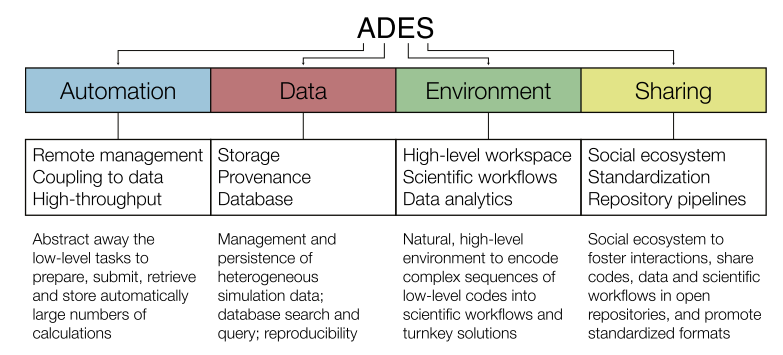
\includegraphics[width=1.0\textwidth]{figs/ch3_ades.png}
  \centering
  \caption{计算科学基础设施工具的四大支柱。在较低的层次上,需要一个自动化框架和一个有效的数据管理解决方案。在用户级别,高级环境与社会生态系统相结合,以促进代码、数据和工作流的共享,图片来源文献\cite{pizzi2016aiida}}
  \label{fig:ch3_ades}
\end{figure}

自动化(A)描述了对底层计算任务参数准备,任务提交,结果检索,计算和数据储存过程封装的自动化过程。 目的是使AiiDA的用户可以简单快速编写自动化的工作流。
\begin{alphaenum}
    \item 远端集群管理。大型的计算通常运行在用户工作站或工性能计算集群上。任务作业的准备、提交、任务状态的查询、计算结果的下载往往独立于计算过程本身,用户会频繁地执行这类操作。因此,这类与远端计算资源交互协作的任务在AiiDA中被抽象为特定的用户程序接口(API)并对各种不同的作业调度系统实现特定插件,以自动化作业的管理过程。
    \item 数据的耦合和解耦。为了确保计算的可重复性,数据的储存和自动化流程需要互相耦合,否则,用户在遭遇计算流程报错时将需要手动尝试解决,而这种人工干预将会使得部分流程无法得到记录,从而丢失数据的完全可重复性。相反的,如果用户在项目中给出了全部的输入,并自动化运行的记录后续全部流程,因其在运行过程中记录数据和数据变化迁移的全部逻辑,就能够确保数据的完全的可重复性。
    \item 高通量计算支持。基于这种自动化的优势,就特定流程的计算,可以变化输入参数,从而对海量的参数进行过滤和扫描以发现最优参数,而这正是高通量计算的主要特征。逐个对海量参数进行运行、分析和过滤是人工难以完成的,借助自动化的工作流可以达到这可目的。
\end{alphaenum}

数据(D),涉及计算模拟数据的产生和数据的管理,涵盖以下三个核心方面:
\begin{alphaenum}
    \item 存储,即储存高性能计算所产生的大量的异质数据。包含输入参数以及最终结果的文件的自动和永久化存储,以便这些数据在将来能够被引用和分析。另一方面,大部分数据只是临时性的,如‘检查点’等,这类数据可以在模拟结束后应该被丢弃。因此,必须采用依赖于计算代码(这里指使用的材料计算的软件如VASP)所需的的文件存储策略(可由用户定制)来对不同输出文件进行分类。在任何情况下,都应该尽可能充分地记录计算模拟过程中产生的中间文件,这样即使在机器重新启动后文件被删除时,计算的逻辑流也能被持久化保存。如果确保了计算模拟的可复现性,那么在需要时重新生成中间文件的流程就很简单了。同时,在生成数据的计算代码上存储信息也很重要。如果需要完完全全的再现性,可以参考使用虚拟机或Docker镜像技术来一并储存完全一样的可执行代码。
    \item 可重复性。为了实现工作流的可重复性(或称为复现性),工具流系统需要存储和表示所执行的计算过程本身及其输入数据。然而,一个有效的数据模型不仅应该强调计算和数据,还应该跟踪它们之间的因果关系,即结果的完整来源。例如,对于弛豫后的晶体结构如果不知道它的初始构型,即是如何获得的最后的结构的,这个情况下结果的用途将很有限。我们使用有向无环图作为表示数据和计算之间关系网络的数据结构。
    \item 数据库。如今常见的计算工作环境通常都由大量具有任意目录结构、任意命名方式和缺乏文档信息的文件组成。在实际应用中,其他用户通常难以清楚地理解和使用这些信息(甚至是数据的创造者自己在一段时间后也对这些数据无能为力),同时大量混乱的数据也使得很难在存储了许多信息后还可以容易地检索特定的计算。数据库可以帮助组织和查询结果。上面所说的基于有向无环图的数据模型的实现,不能局限于特定的应用程序,而还必须适应异构数据。它必须能够有效地查询与图形节点相关联的任何属性的信息(包括但不限于数字、字符串、列表、字典等)。另外的,遍历图以评估节点之间因果关系的查询也是必要的。如果满足上述要求,就不需要图形数据库作为后端。例如,AiiDA的后端是一个关系数据库,可用于有效的图遍历。
\end{alphaenum}

上面描述的前两个动机主要针对底层的功能。接下来的两大设计动机则是面向用户端的功能实现。其中,环境(E)侧重于为计算科学创造一个社群环境,涉及以下几个方面:

\begin{alphaenum}
    \item 具象和可直接使用的工作界面。由于研究人员的目标是进行新的研究发现,而不应止步于学习新的代码,因此面向用户的基础工具应该灵活且易于使用。例如,尽管数据库在数据驱动的计算科学方面提供了许多优势,但很少有科学家是该方面的专家。因此,数据库管理和连接的复杂性必须通过API抽象层来充分隐藏。此外,通过使用广泛使用的高级编程语言(如AiiDA采用的Python),人们可以受益于各种成熟的已经存在的能够用于从数据库插入和检索数据的工具。同时基础工具也必须是模块化的,以提供通用的底层功能核心,以及支持不同计算模拟软件代码的可定制插件的编写。
    \item 科学工作流。许多科学知识不仅存在于最终保存的数据中,还存在于对过程的描述中,即那些用来生成这些数据的“科学工作流程”。如果可以对这些流程进行编码储存,那么就可以在需要的时候重用它们,并用来在不同的情况和条件下计算相似的结果(如仅仅改变流程中的个别参数)。工作流指定了计算步骤之间的依赖关系,依赖关系可能不是在开始时就定义号的的,而是有可能依赖于中间结果(例如,计算材料学中常见的迭代次数未知的迭代收敛)。因此,基础工具应该只有在前面的步骤结束后动态地根据结果生成后续的计算,并在运行时重新生成完整的依赖关系。科学工作流与其他基础设计动机相配合,帮助用户专注于工作流逻辑,而不是对远程集群的管理使用的细节。一个额外的好处是,在工具执行期间能够自动存储数据来源并生成了一个隐含的有关结果数据逻辑的文档。
    \item 数据分析。应用驱动的计算材料学研究往往需要使用数十种不同的工具和近似方法。然而,用不同代码得到的结果往往都有相同的后处理或可视化算法。这些数据类型(例如晶体结构或带结构)应该以相同的公共格式存储。然后,再通过基础工具来提供数据分析的功能来执行相应的操作,或者充分使用已有的成熟的工具或软件库。这可以通过提供数据处理和分析的外部工具接口来实现(例如晶体结构\cite{ong2013python}),而不需要考虑用于生成数据的具体模拟计算软件代码。
\end{alphaenum}

第四个设计动机是共享(S),我们目标创建一个计算材料的生态系统,以促进科学家之间的互动,特别是共享数据、结果共享和科学工作流程共享。

\begin{alphaenum}
    \item 生态系统。指的是工具的框架应该是一种能够在计算材料研究中能同时创建生态系统的技术,同时需要非常小心地考虑数据访问策略。研究人员有时更喜欢保持他们的数据的私密性(同时保护正在申请的专利或未发表的数据),但如果需要与合作者或公共存储库共享,应该通过很小的努力就可以实现数据保密层级的变化来共享数据。除了数据共享,还应该提供一个标准化的插件接口,使得插件易于编写和设置。用户可以容易地贡献共享工作流,处理新的数据格式,或支持新的计算模拟软件代码。通过这种机制,科学家将能够进行社区型的计算和保证数据共享,这与移动应用程序和网络生态系统的发展并行。
    \item 标准化。为了促进数据交换,研究者之间应商定并采用标准格式来共享数据\cite{murray2003chemical}。即使存在多个不同标准,也可以设想一个可选择的配置,其中每个新计算代码都以既定格式提供数据。另一方面,定义合适的数据实体也很重要(例如,简化要存储在给定数据库中的物理量的名称和物理单位,以及它们的含义)。特定于领域有其特定的数据实体,其定义必须是社区驱动的(如TCOD\cite{merkys2017posteriori}数据库)。基础工具在这方面将很有用,既可以作为数据实体的生产来源,也可以作为生产包含一组模拟用例的测试环境。
    \item 数据仓库。随着存储仓库的出现,直接导入或导出数据的能力(通过REST接口或通过适当协议)变得很重要。如果建立了格式和数据实体,平台必须简单地将数据及其来源转换为指定的格式。这使得对外部数据库的贡献变得非常简单,同时平台也能成为创建共享存储库的促进者。
\end{alphaenum}

\subsection{AiiDA内核的架构设计}

AiiDA在设计上能够广泛适用于各种计算规模的计算科学问题和各种计算能力的计算应用,但其最主要的应用还是对高性能计算(HPC)系统的支持。HPC的用户通常习惯通过脚本来使用计算资源,因此AiiDA的工作流引擎提供了一个丰富的应用软件接口(API)以编写工作流,而非像其他主流工作流管理系统,如Kepler\cite{altintas2004kepler}, Taverna\cite{oinn2004taverna},  和Triana\cite{taylor2003triana},通过提供图形用户接口(GUI)来定制工作流。API能够更加明晰地、无缝地将工作流系统与在高性能计算机上运行的模拟计算代码以及数据处理分析工具结合,从而让用户有最大的自由度来构建符合其目的的合适的工作流。需要说明的是,这种灵活性是以牺牲用户的学习成本实现的,用户需要编写一些简单的脚本,来使用AiiDA构建工作流。但对于已经习惯通过脚本来使用HPC的用户,这样的学习成本非常之小。

基于API的工作流定义方式的另一个优势是,能够定义动态的工作流。动态工作流指的是运行路径并非提前定义并固定的工作流,而是会随着工作流的执行运行时地动态变化执行逻辑的工作流。
最显而易见的例子是计算流程的错误处理与恢复。在AiiDA中,定义工作流的代码是被其引擎直接运行,而不通过中间层,这点与多数工作流管理系统区别,它们通过静态的标记语言如XML或通用工作流语言(CWL)\cite{amstutz2016common}来定义工作流,然后转化为无环图(DAG)的形式以供运行。
静态工作流的最大劣势也就是动态工作流的最大优势,就是整个工作流的运行步骤是不需要提前确定的,这使得编写有程序逻辑的工作流成为可能。

AiiDA的软件架构理论上很好的反映了针对高通量计算材料学所追求的目标。包括运行设备的可拓展性,即可以在小型个人电脑上运行也能在高性能计算集群上运行以及可以运行各种时间范围的任务,小到仅需几秒钟完成的小型处理型任务,大到需要几周时间完成的运行在高性能集群上的任务。另外,它能在一个设备上同时处理成千上万这样的进程。开发中时,AiiDA被设计为安装运行在用户的个人工作站上,但在实际生产环境中AiiDA可以被一群人通过多用户的方式一起使用,甚至能够运行在如Material Cloud\cite{talirz2020materials}这样的公共平台上。

如图\ref{fig:client-worker}所示,工作流引擎依赖使用以下两个外部组建来运行工作流:
\begin{alphaenum}
    \item 数据库引擎(PostgreSQL\cite{postgresql}),用于保存每个进程的当前运行状态。并且该数据库还充当了向用户展示进程运行状态的功能。
    \item 消息中间件组建(RabbitMQ\cite{rabbitmq})用于在客户端和服务端之间传输有关进程状态的消息
\end{alphaenum}
这些组建即可以运行在AiiDA内核所运行的机器上,也能运行在独立的一个服务器上。通过这样层级的解耦,开发中和使用时的效率被大大提升。

\begin{figure}
  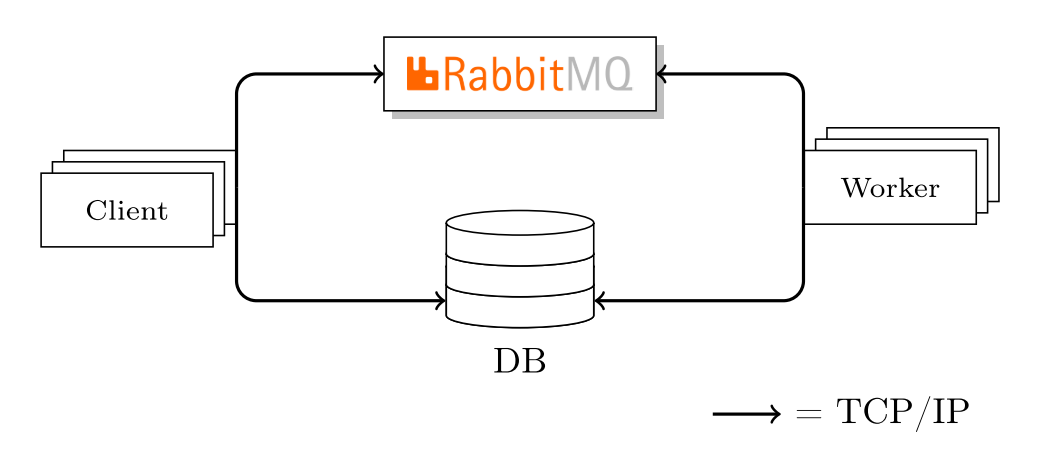
\includegraphics[width=1.0\textwidth]{figs/db-rmq.png}
  \caption{客户端和运行端通过TCP/IP连接到数据库和RabbitMQ服务,支持丰富的可能配置和相应的使用场景。守护进程在一个单独的Python进程(称为worker)中管理多个并发的运行程序。每个运行器串行执行,但仍然能够在使用Python协程等待进程时通过切换槽来处理多个AiiDA进程。}
  \label{fig:client-worker}
\end{figure}

为了能够在设计上满足工作流系统响应性、可拓展性、支持高通量的目标,我们极大的依赖于通过事件触发作为进程运行中的进程控制信号。比如当一个工作流在运行中等待远端完成任务时,或者当向运行的进程发送一个终止信号后等待其完全关闭的过程中,所有的进程的状态转换都是通过进程相关的状态机的事件来触发的。这种涉及和基于等待队列的系统(如集群端的大部分任务调度系统)形成对比,等待队列的系统拥有一个管理进程的池,在进程运行时通过不断的查询进程状态来改变和触发后续要执行的动作。这种系统在高性能集群的任务调度系统中使用较多,因为集群上的任务往往都有较长的运行时间。但这种进程管理的触发后续任务的方式的响应性较低,不符合我们在运行高通量计算处理快速进程时要求快速响应的特点。

与其他的基于事件的系统如用户界面系统、计算机游戏等类似,AiiDA使用事件循环来实现这一目标,我们选择使用\texttt{asyncio}这一Python自带的并发库来实现这一目的。这使得多个AiiDA进程可以通过一个单独的Python进程进行管理,尽管没有多线程的支持,异步运行的协程之间还是能够合理的被调度和运行,在等待外部设备读写的过程中可以快速地将计算机进程的使用权交由其他协程来处理。使用协程而非线程技术来处理多任务的共同运行还解决了数据库读写的负载问题,因为默认的数据库服务器的连接数通常不多,如PostgreSQL默认仅支持100个连接。
而且,使用多线程来编程非常的反直觉并且难以开发调试,即便是对于经验丰富的程序员针对多线程的开发调试也是非常困难的,特别是在AiiDA中因为我们对如何调用API没有施加过多的特殊限制因此更增加了多线程开发的难度。

执行工作流所需的全部Python组件都集中在\texttt{Runner}类中,该类提供事件循环、状态记录、传输(例如SSH)以及一些其他功能,其中一些功能将在下面进行更详细的描述。由于使用了事件循环,每个运行器(Runner)可以并发地运行内存限制内任意数量的工作流进程。我们把可以在单个运行程序上运行的进程数称为任务槽数。

运行器可以在本地终端中独立使用。但在大多数生产环境中,用户希望启动一个,可以管理一个或多个运行程序的守护进程,同时支持在运行程序崩溃时通过守护进程自动重新启动。在AiiDA中,我们使用\texttt{circus}库\cite{circus}来实现这一功能。\texttt{circus}提供了启动多个运行系统进程的功能,当运行的进程崩溃时,\texttt{circus}会记录并按照用户定制的方式自动重新启动终断的进程。此外,它还可以显示有关进程运行所需要的当前资源使用情况的信息,并可以支持动态增加运行时池中运行的系统进程的数量。

\begin{figure}
    \centering
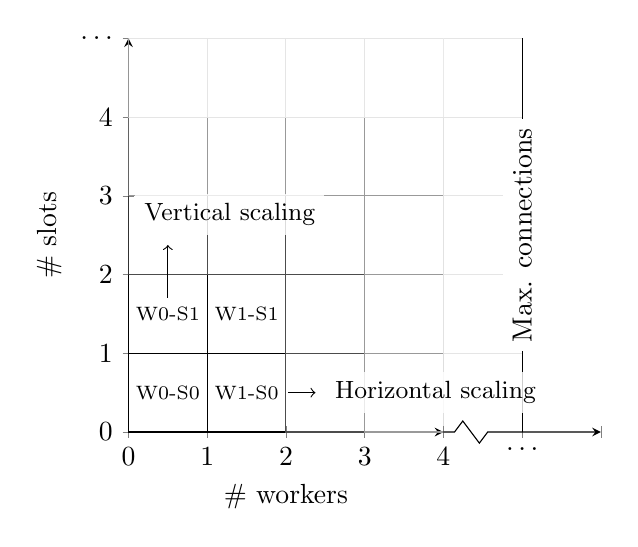
\begin{tikzpicture}[auto]

\begin{groupplot}[
    group style={
        group size=2 by 1,
        xticklabels at=edge bottom,
        horizontal sep=0pt
    },
    axis lines = left,
    ylabel = {\# slots},
    ymin=0, ymax=5,
    xmin=0, xmax=101,
    ytick={0, 1, 2, 3, 4, 5},
    yticklabels = {0, 1, 2, 3, 4, $\ldots$},
    scale only axis,
]
\tikzstyle{cell} = [execute at begin node=\scriptsize, text centered, anchor=center]
\nextgroupplot[
    xmin=0,xmax=4,
    ymin=0,ymax=5,
    width=4cm,
    height=5cm,
    xlabel = {\# workers},
]
\draw (axis cs: 0,0) rectangle node[cell] {W0-S0} (axis cs: 1,1);
\draw (axis cs: 0,1) rectangle node[cell] (w1s2) {W0-S1} (axis cs: 1,2);
\draw[color=black!70] (axis cs: 0,2) rectangle node[anchor=center] (w1s3) {} (axis cs: 1,3);
\draw[color=black!40] (axis cs: 0,3) rectangle (axis cs: 1,4);
\draw[color=black!10] (axis cs: 0,4) rectangle (axis cs: 1,5);

\draw (axis cs: 1,0) rectangle node[cell] (w1s0) {W1-S0} (axis cs: 2,1);
\draw (axis cs: 1,1) rectangle node[cell] {W1-S1} (axis cs: 2,2);
\draw[color=black!70] (axis cs: 1,2) rectangle (axis cs: 2,3);
\draw[color=black!40] (axis cs: 1,3) rectangle (axis cs: 2,4);
\draw[color=black!10] (axis cs: 1,4) rectangle (axis cs: 2,5);

\draw[color=black!70] (axis cs: 2,0) rectangle node[anchor=center] (w3s1) {} (axis cs: 3,1);
\draw[color=black!70] (axis cs: 2,1) rectangle (axis cs: 3,2);
\draw[color=black!70] (axis cs: 2,2) rectangle (axis cs: 3,3);
\draw[color=black!40] (axis cs: 2,3) rectangle (axis cs: 3,4);
\draw[color=black!10] (axis cs: 2,4) rectangle (axis cs: 3,5);

\draw[color=black!40] (axis cs: 3,0) rectangle (axis cs: 4,1);
\draw[color=black!40] (axis cs: 3,1) rectangle (axis cs: 4,2);
\draw[color=black!40] (axis cs: 3,2) rectangle (axis cs: 4,3);
\draw[color=black!40] (axis cs: 3,3) rectangle (axis cs: 4,4);
\draw[color=black!10] (axis cs: 3,4) rectangle (axis cs: 4,5);

\draw[color=black!10] (axis cs: 4,0) rectangle (axis cs: 5,1);
\draw[color=black!10] (axis cs: 4,1) rectangle (axis cs: 5,2);
\draw[color=black!10] (axis cs: 4,2) rectangle (axis cs: 5,3);
\draw[color=black!10] (axis cs: 4,3) rectangle (axis cs: 5,4);
\draw[color=black!10] (axis cs: 4,4) rectangle (axis cs: 5,5);

\draw[->] (w1s0) -- (w3s1);
\draw[->] (w1s2) -- (w1s3);

\nextgroupplot[
    xmin=99, xmax=101,
    ymin=0, ymax=5,
    xtick = {99,100,101},
    xticklabels={,$\ldots$,},
    axis y line=none,
    axis x line=middle,
    axis x discontinuity=crunch,
    height=5cm,
    width=2cm
]

\draw[color=black!10] (axis cs: 99,1) rectangle (axis cs: 100,2);
\draw[color=black!10] (axis cs: 99,2) rectangle (axis cs: 100,3);
\draw[color=black!10] (axis cs: 99,3) rectangle (axis cs: 100,4);
\draw[color=black!10] (axis cs: 99,4) rectangle (axis cs: 100,5);

\draw (axis cs:100,0) -- (axis cs:100,6);
\node[rotate=90,fill=white,anchor=center] at (axis cs:100,2.5) {Max. connections};

\end{groupplot}

\node[anchor=south west, xshift=-12pt,fill=white,fill opacity=0.8,text opacity=1] at (w1s3) {\small Vertical scaling};
\node[anchor=west,fill=white,fill opacity=0.8,text opacity=1] at (w3s1) {\small Horizontal scaling};


\end{tikzpicture}
    \caption{
    每个runner中worker的数量和插槽数量的变化范围。可接受的并发的AiiDA过程的总数是两个坐标轴上的值的乘积
    }
    \label{fig:daemon-scaling}
\end{figure}


使用这个守护进程,如图\ref{fig:daemon-scaling}所示,你可以垂直扩展(每个runner有多个插槽)和水平扩展(多个Python实例,每个实例有一个runner)。对于需要大量python内处理的工作负载,最好在工作时扩展worker的数量——涉及许多远程计算的负载可以扩展每个worker的插槽数量,从而实现在运行守护进程的计算机上最小化负载系统资源减,少吞吐量的损失。当worker的数量等于数据库连接的最大数量时,就达到了限制上限,用户无法再增加运行对象,但如果用户能够访问数据库设置,那么这个数据库相关的上限是可配置的。

AiiDA工作流引擎运行时的主要工作对象是\texttt{Process}类。
所有其他类如\texttt{WorkChaian}类、\texttt{CalcJobs}类等)都是从\texttt{Process}(或其子类)派生而来的,因此继承了大量原始类的常见功能和特性。\texttt{Process}类本身是为一个扩展的状态机,这意味着由一个有限状态机组成,如图\ref{fig:process_state_machine}所示,其中每个状态都可以有内部数据作为其扩展状态的一部分。
这是事件驱动系统中常见的模式,因为它提供了统一的方式来定制特定状态,以及触发事件的动作,这些事件触发动作(hook)可以用作触发器,在状态转换期间执行流程特定的内部逻辑或外部数据交换等操作。
事件触发动作本身以\texttt{Process}类的成员函数形式定义,比如:

\begin{lstlisting}[
    language=python,
    label=code:state-transition-hooks,
    caption={AiiDA中 \texttt{Process} 类状态转移时的事件触发。
    这对于确保在发生状态转换时执行某些操作是非常重要的。},
]
# Entering a new state
def on_entering(self, state):
    ...

# Just entered the new state from 'from_state'
def on_entered(self, from_state):
    ...

# About to exit the current state
def on_exiting(self):
    ...
\end{lstlisting}

通过使用这些事件触发器,可以有选择地在状态转换的不同时刻执行相应的动作,如上面例子中,\texttt{on\_entered}触发后保证了完成后的状态一致。
这些触发器在AiiDA中的一个重要用途是,它能够将进程的当前状态反射回数据库,同时包括了记录和保存当前进程的检查点状态及信息。
状态转换触发器还可以用于发送广播消息,允许接受客户端(可能位于远程机器上)在当前进程状态更改时更新它们在数据库中的状态信息。

\begin{figure}
\center
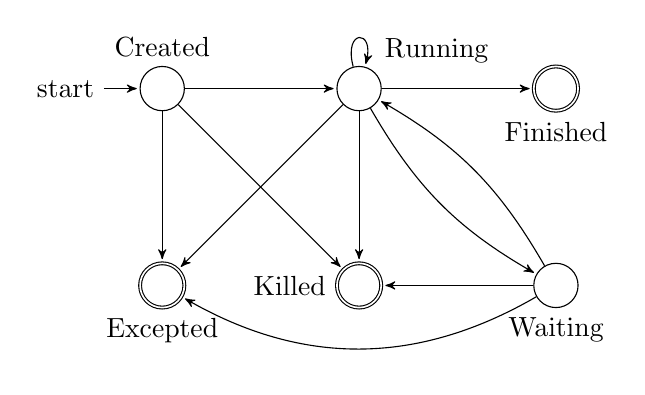
\begin{tikzpicture}[>=stealth',shorten >=1pt,auto]
%                   ___
%                  |   v
%     CREATED --- RUNNING --- FINISHED (o)
%                  |   ^     /
%                  v   |    /
%                  WAITING--
%                  |   ^
%                   ----


%       * -- EXCEPTED (o)
%       * -- KILLED (o)
    \tikzstyle{every state}=[node distance=2.5cm, font=\tiny, minimum size=16pt]
    \node[state,initial,label=above:{Created}] (created) {};
    \node[state,right of=created, label=above right:{Running}] (running) {};
    % Terminal states
    \node[state,accepting,right of=running, label=below:{Finished}] (finished) {};
    \node[state,accepting,below of=created, label=below:{Excepted}] (excepted) {};
    \node[state,accepting,below of=running, label=left:{Killed}] (killed) {};

    \node[state,below of=finished, label=below:{Waiting}] (waiting) {};


    \path[->] (created) edge (running)
              (running) edge (finished)
              (running) edge [loop above] (running)
              (running) edge [bend right=15] (waiting)
              (waiting) edge [bend right=15.] (running);

    \path[->] (created) edge (killed);
    \path[->] (running) edge (killed);
    \path[->] (waiting) edge (killed);

    \path[->] (created) edge (excepted);
    \path[->] (running) edge (excepted);
    \path[->] (waiting) edge[bend left] (excepted);
\end{tikzpicture}
\caption{
  进程状态机。
  终止状态用一个套叠的圆环表示。
}
\label{fig:process_state_machine}
\end{figure}

一个完整的进程通常会经过各种状态,可能在状态转移时分别运行几个成员函数或等待其他进程完成。
但是,如果进程中发生异常,则该异常会被捕获,运行器(Runner)将会把进程转换到终端例外状态,并同时创建一个日志条目,以包括对Python堆栈信息的跟踪。
而另一种手动使进程提前终止的方法是调用\texttt{kill}成员方法,来使进程进入终止状态。

引擎在实现中的一个重要设计是,进程的运行是具有检查点和可以被持久化保存的的。
这样,在有意或无意关闭进程的情况下,AiiDA可以在引擎重新启动后从最后的被保存的正确运行时状态恢复并继续运行,从而实现了计算机的关闭(断电或人为关机)不会影响长时间的任务进程的良好运行。
为了实现这一点,我们使用了在进程状态转换时将检查点及相应进程信息写入数据库。
具体来说,任务进程的相关上下文信息、输出和特定的元数据将会被保存到一个字典数据结构中,然后由AiiDA构建特定的持久化保存的数据结构存入数据库中,整个检查点的持久化储存的方式如图\ref{fig:persister}所示。

\begin{figure}
  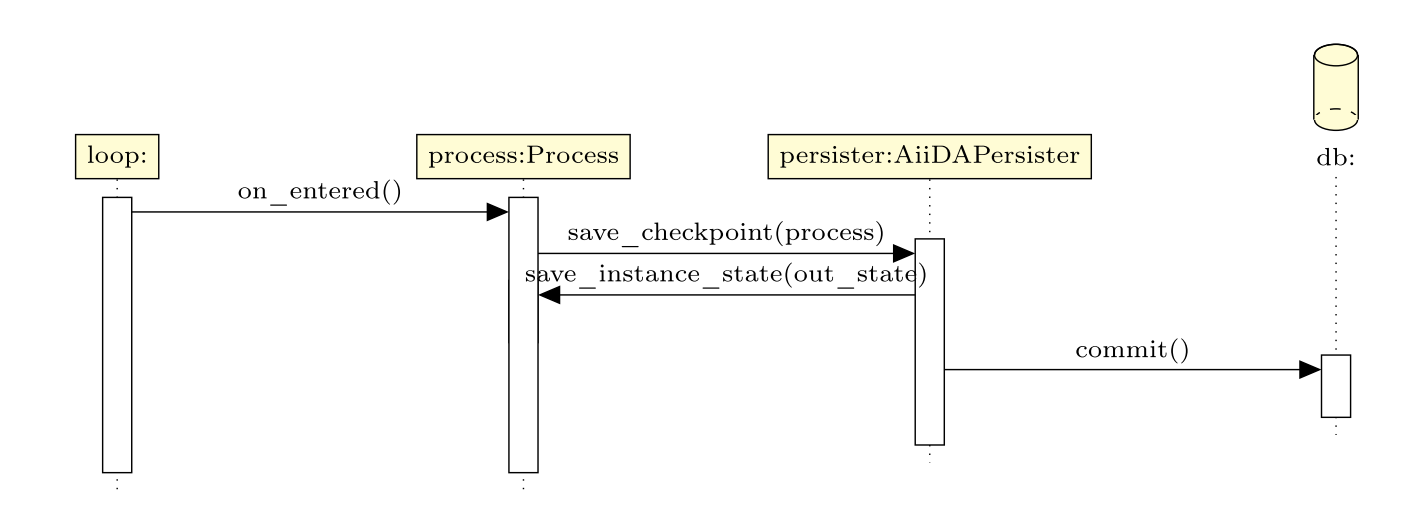
\includegraphics[width=1.0\textwidth]{figs/persister.png}
  \centering
  \caption{显示在状态转换时流程的内部状态的持久性的UML活动图。竖条显示实体(顶部)活动期间的时间,因此定义了它的范围。当持久化进程获得保存检查点的请求时,它调用进程并请求它生成一个字典,即\texttt{out\_state},然后将其序列化并提交给数据库}
  \label{fig:persister}
\end{figure}

工作流引擎主要通过消息传递来对流程进行外部控制,并以此在确保容错的同时保持高吞吐量。
而消息传递是通过使用被称为消息中间件的组件实现的,在我们的例子中使用了RabbitMQ这一开源的消息中间件组件。
消息中间件通常负责保证消息的持久性和独立性,通过与应用程序内部逻辑解耦来使应用程序内部仅关注其相应的业务逻辑。
在RabbitMQ中,用户需要首先在服务端安装并打开一个消息传递服务,再使用客户端软件通过TCP端口进行消息交互。消息的路由和信息持久化保存均是由RabbitMQ内部处理实现的,这大大简化了我们开发的工作量。

为了方便AiiDA与RabbitMQ交互,我们开发了一个Python库kiwiPy, kiwiPy依赖\texttt{aio\_pika}库实现和RabbitMQ的交互。KiwiPy最大可能模拟并封装了与RabbitMQ的主要交互过程,并提供了将通信信息装在到单独线程的功能。这中封装对于AiiDA来说至关重要,详细信息请参考接下来的有关任务队列的小节。同时,除了任务队列外,kiwiPy还为AiiDA提供发送远程函数调用(RPC)和广播消息的能力。

任务队列用于安排和调度要运行的新进程。使用RabbitMQ的一个主要的优势是它能够根据所选择的设置提供了一定的消息成功传输的保证。
对于我们的任务队列,AiiDA使用持久化的消息,这些消息被持久化保存到磁盘中,以便在机器有意或无意地重新启动后仍然存在并可以恢复到机器关闭前的状态。
因此,作业一旦从客户机交付给代理,就需要确保永远不会丢失。此外,RabbitMQ还需要告知已经完成的任务,因为如果它失去了与worker的连接,它需要能够自动重新将任务排到队列中,直到确认任务执行完成。
这种机制依赖于周期消息这一组件,一般也被称为心跳包, worker必须在设定的时间周期内及时作出响应,否则,当连续两个心跳包响应丢失时,RabbitMQ会认为worker已经中止运行,并触发重调度机制。
也是因为这个原因,kiwiPy额外地运行在一个独立的线程中(与其他真实的任务独立),以此确保即使AiiDA进程在一个有极大的阻塞的工作负载下,它也能够正常地响应心跳。

RPC全称为Remote Procedure Call即远程函数调用。正如其名称所暗示的,这些类型的消息用于调用特定过程(在我们的例子中是函数或类的方法),并将过程的结果传递回给调用者。
这主要用于暂停、执行和终止特定的活动进程。

广播功能涉及到向任意以定义的侦听器发送单个消息,它们不需要收到特定的响应。该模式主要有两个目的,分别是暂停、执行或终止包含多个进程的进程组,并控制它们之间的信息流。已经产生子进程的父进程可以选择等待子进程完成后再继续执行。父进程通过将自己注册定义为子进程广播的监听器,当它接收到子进程终止消息时,父进程可以方便地实现对进程终止。这种机制使AiiDA中\texttt{to\_context}的工作链构造的功能得以实现,即当工作链中的进程可以通知工作链当它所等待的流程完成时该进程可以继续进行。

%
% %\chapter{不等价结构的生成和查重算法}
\chapter{不等价结构的生成和查重算法}
通过第一性原理来计算和预测材料的热力学稳定的构型是计算材料学近几十年的一个重要发展。尽管这个问题很困难,但由于其重要的应用价值它吸引力许多的研究关注。因为计算过程的自由度和搜索的空间十分巨大,简单的结果往往需要对及其大量的材料构型进行计算,同时又因为第一性原理的能量计算的计算资源耗费较大,这个问题变得十分困难。这个问题被称作晶体结构预测问题(CSP),近些年发展了非常多的方法来解决这一问题,我们在第\ref{chapter:workflows}章中已经简要介绍了相关的全局材料搜索和高通量的材料搜索方法。

这一章我们主要介绍晶体结构预测问题(CSP)的子集,即在晶格类型已知的构型中的晶格体结构预测问题的算法和实现。这个问题虽然是原问题的子集但它同样非常重要,实验发现许多半导体或金属间形成的合金都是通过这种固定的晶格的形式形成合金。我们通过自己编写的软件用于实现了产生不等价的结构,并使用到了本论文的相关工作中。枚举产生的不等价的结构后续会被用到完整的用于确定热力学稳定性的搜索过程。

\begin{figure}
  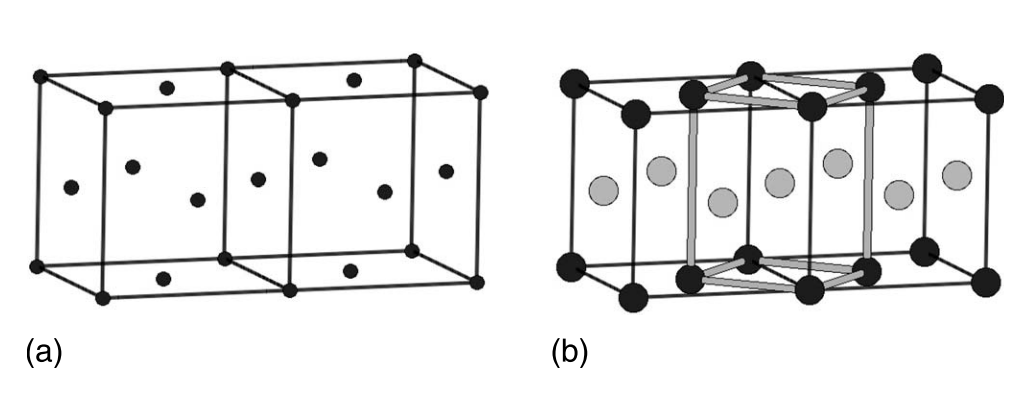
\includegraphics[width=0.72\textwidth]{figs/ch4_fcc_superlattice.png}
  \centering
  \caption{左边是原面心立方晶格,右边是原晶格扩充的超晶格,超晶格是由灰色的双单元格定义的。超晶格的两个内部点被一个黑色原子和一个灰色原子所占据。超晶格和原子一起构成了一种衍生结构。这个例子的所对应的真实合金是\ce{CuAu}合金。}
  \label{fig:ch4_fcc_superlattice}
\end{figure}

合金中的化学序结构,磁性材料中的磁序结构,以及非化学配比的带有缺陷序的材料表现出各种不同的性质都与其原超结构的衍生结构\cite{buerger1947derivative,santoro1973coincidence,santoro1972properties}有关。同样的还有超晶格的衍生结构,是孪晶中影响结构和性质的重要因素之一。那么什么是超结构的衍生结构呢?这里我们定义其为单胞是其原单胞数倍拓展而来,原子坐标的基矢是原单胞对应的向量加和,但原子排列不同于原单胞的构型。比如许多金属间化合物可以认为是由面心立方而来的超结构,如图\ref{fig:ch4_fcc_superlattice}所示,(b)中的构型的原子占有面心立方晶格所处的原子处,但因为其有两种原子所以不再有面心立方的对称性,而成为面心立方结构(图\ref{fig:ch4_fcc_superlattice}(a))的衍生的超结构。图\ref{fig:ch4_fcc_234_ss}中展示了面心立方晶格的两倍三倍,四倍超胞的各种晶格以及所拥有的衍生超结构。

\begin{figure}
  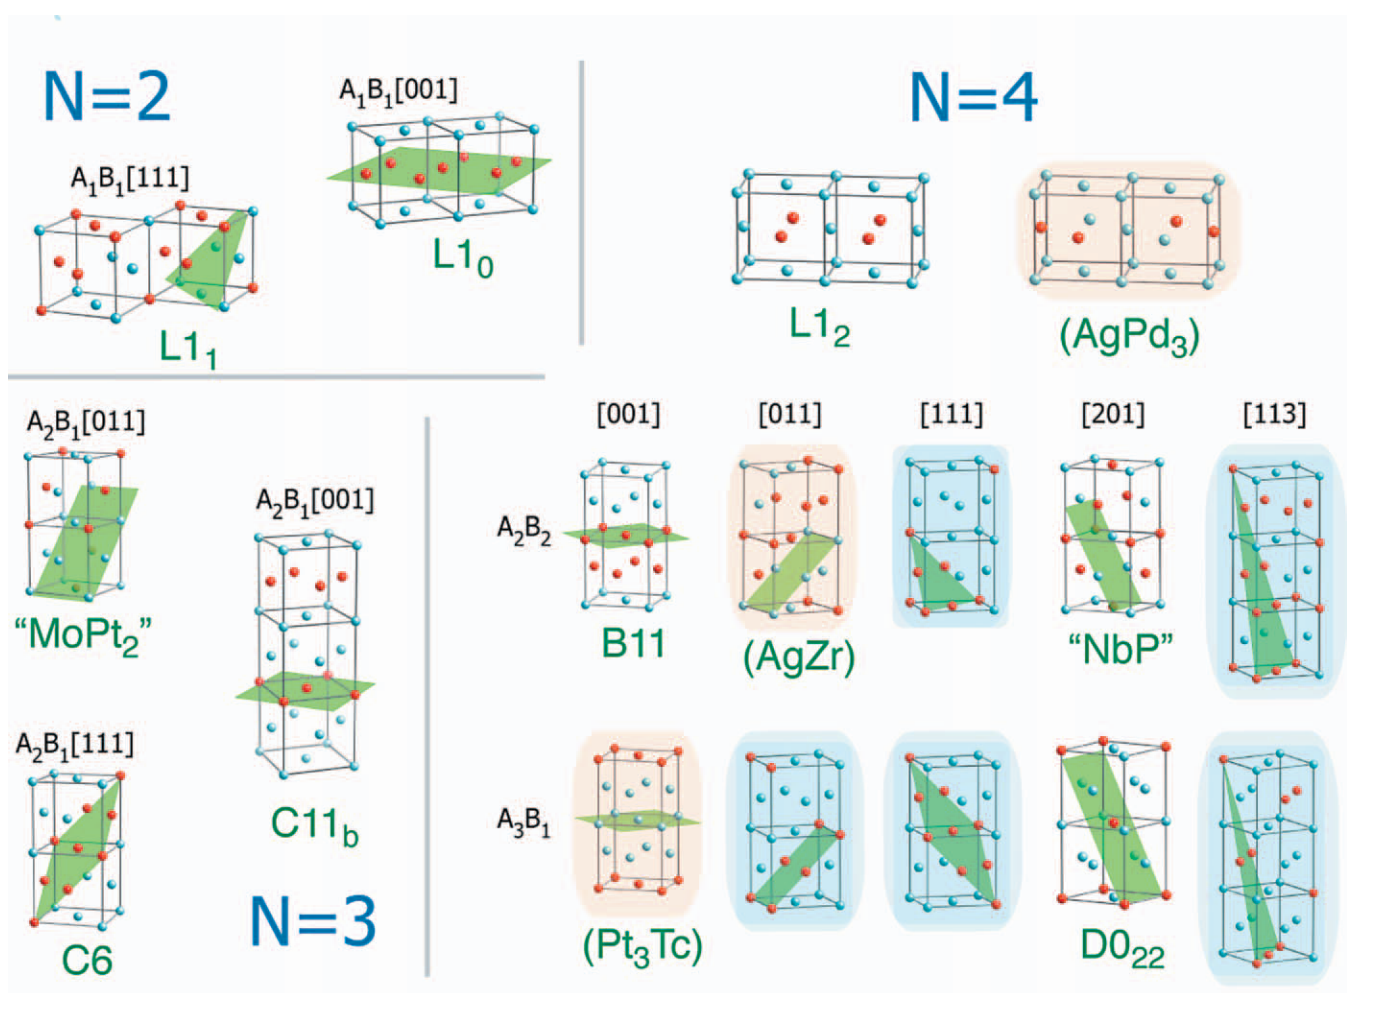
\includegraphics[width=0.96\textwidth]{figs/ch4_fcc_234_ss.png}
  \centering
  \caption{来源于面心立方晶格的前17种二元结构。超胞体积胞为原胞的二倍三倍或四倍。绿色平面所示的结构可以看作由纯A和B原子层叠加而成。例如,左上角的$L_{10}$结构是一个交替的\ce{A1B1}层序,沿001方向堆叠。所有的二倍和三倍于原晶胞的结构都有实际的物理材料的对应。在四倍的超晶格中,有4种构型具有实际的物理材料对应。其他三个黄色背景的构型已经被文献\cite{curtarolo2005accuracy}预测存在,但还没有被实验合成。另外五种蓝色背景的构型是从未被观测到或预测存在于任何系统中的。图片来源文献\cite{hart2008algorithm}}
  \label{fig:ch4_fcc_234_ss}
\end{figure}

生成的衍生结构的集合通常会被用于如确定固定晶格的二元金属间合金的基态性质。同时该方法也不仅限于搜索构型的能量,只要能够定义和有序构型有关的哈密顿量,就能描述其他的物理性质,比如Graf等\cite{graf2005direct}通过定义经验赝哈密顿量来直接预测半导体合金的带系和有效质量。只要所需要的物理性质和衍生结构构型是有关联的,就可以通过这种构建赝哈密顿量方法来建立构型和性质的联系从而搜索并预测合金的性质。

我们先简要概述所用到算法的逻辑框架,再在以下小节详细叙述算法细节。大体上枚举查重算法分为两步,1)产生不重复的超胞,2)对特定超胞产生不重复的编号(即在晶胞对应的旋转和平移操作后不重复的编号)。

第一步晶胞的查重是通过使用厄米标准型的整数矩阵来表示由基础单胞扩充而来的超胞,从而由厄米标准型的唯一性来表示并避免周期性对称下相同超胞的不同表示所造成的重复。我们首先对给定的行列式值(代表超胞的体积)产生所有的厄米标准矩阵。因为物理上晶体具有旋转的对称操作,这些矩阵所对应的超胞有部分是可以通过旋转操作等价的。通过对比旋转操作后的晶体的等价性,我们去除所有重复的超胞仅留下一个代表结构。如图\ref{fig:ch4_2d_square_lattice}所示,(a)中是所有可能的厄米标准型矩阵对应的超胞,(b)是去除物理等价的超胞后的不等价的超胞。

\begin{figure}
  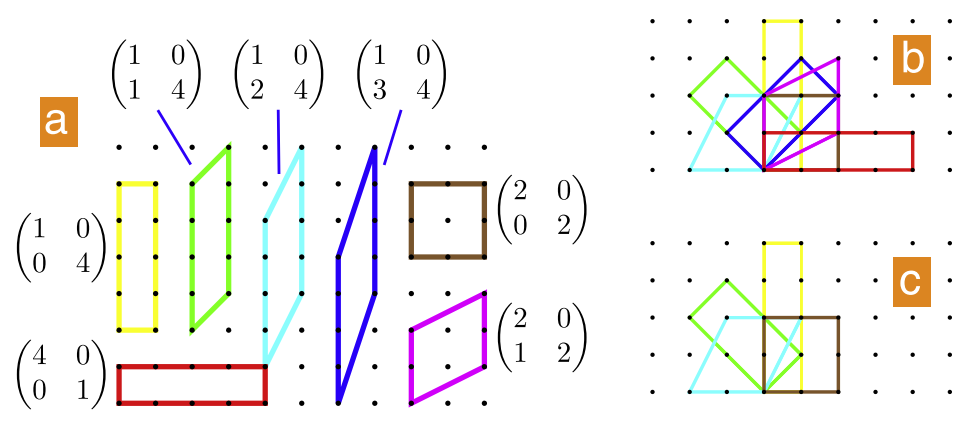
\includegraphics[width=0.86\textwidth]{figs/ch4_2d_square_lattice.png}
  \caption{(a) 7个大小为四倍原晶格的厄米标准型(HNF)基矢量及其对应的单位晶胞。(b)相同的超晶格,但使用最短的(正交的)基向量来描述。(c)这七个晶格去重后的四个完全不等价的超晶格。}
  \label{fig:ch4_2d_square_lattice}
\end{figure}

第二步对于特定的超胞,格点位置可以放置不同的种类的原子构成不同的构型,两个构型之间是否相同可以通过对一个构型施加晶胞对应的所有操作后对比另外一个结构检查是否等价。在实际操作中,对结构直接作用对称操作得到新的空间坐标的计算效率并不高,因为针对的是确定格点的结构,格点间的距离是一个多余的参量,不影响等价性的结果,因此可以对特定超胞的不同晶格进行编号,则超胞的商群中的每一个对称操作都会等价于一个置换操作。以二元合金为例,每个构型都可以由一个二进制0,1编号表示,因此可变换对应于一个十进制整数,每一个对称操作所产生的效果仅仅是将一个整数变为另一个整数,我们通过哈希表来储存所有无法通过对称性变换到集合中其他对象的所有非等价的对象。

下面小节详细描述这两步所涉及的细节内容。

\section{晶胞的查重}
晶胞查重的第一步是给出所提供的原始晶格的所有平移不等价超晶格(可包含因旋转操作而重复的晶格),即产生所有的衍生晶胞的初始非平移等价的集合。我们考虑$B=A\cdot H$,这样的晶胞变换,其中$A$是原始晶胞的基矢(为表述清晰,论本表述中使用列向量的形式,但在程序中有时会使用置换操作变为行向量表示晶胞的基矢),$H$为作用在原始矩阵的变换矩阵,其元素为整数,$B$则为变换后的基矢。如果$H$是一个行列式为\num{+-1}的矩阵,则变换后的晶胞与原晶胞物理等价,$A$和$B$仅仅是同一套晶胞对应的不同的基矢选择。换言之,如果整数$H$矩阵的行列式为\num{2},则晶格$B$是晶格$A$的超晶格,且为单胞体积其原晶格单胞体积的两倍。

我们设有两个整数矩阵$H_1$,$H_2$有相同的行列式值,如果$H_1$能够通过整数的列操作(列之间的线性运算)变为$H_2$,则他们产生的是同一套晶格。我们将这些操作矩阵的正则形式表示为下三角矩阵的厄米标准型形式,这样能够保证每个超晶格都有且仅有一个矩阵对应(下三角厄米标准型的唯一性\cite{santoro1973coincidence})。三维情况下,下三角矩阵厄米标准型为:

\begin{equation}\label{eq:hnf}
  \begin{pmatrix}
    a & 0 & 0 \\
    b & c & 0 \\
    d & e & f
  \end{pmatrix}, \qquad
  0\leq b < c, \qquad
  0\leq d, e< f.
\end{equation}

这种表示下,矩阵的行列式的值为对角线元素的乘积$a\times c \times f$。同时,该行列式值n也是拓展后超晶格的体积,即将原始晶胞体积看作1时变换后的单胞的体积倍数。在这样的定义下,所有的矩阵的超晶格对应的矩阵都能够通过指定行列式的值后确定行列式分解为三个整数的乘积形式,再通过式(\ref{eq:hnf})来限制$b$,$d$,$e$的值,从而构造能将原始晶格变换为超晶格的唯一平移不等价的变换矩阵$H$。

综上,给定$H$矩阵的行列式值后枚举所有的H矩阵的算法非常简单,共包含两步:首先,找到$H$行列式的其中一个因数$a$,并保证$1\leq a \leq |H|$,以及第二个对角线因数$c$满足$1\leq c\leq |H|/a$,以及$f$满足$1\leq f\leq |H|/(ac)$。我们以行列式为\num{6}的变换矩阵为例,共可以得到如下表中的所有对角线元素$a$,$c$,$f$的组合。

\begin{table}
  \centering
  \begin{tabular}{c|ccccccccc}
    a & 1 & 1 & 1 & 1 & 2 & 2 & 3 & 3 & 6 \\
    \hline
    c & 1 & 2 & 3 & 6 & 1 & 3 & 1 & 2 & 1 \\
    \hline
    f & 6 & 3 & 2 & 1 & 3 & 1 & 2 & 1 & 1 \\
  \end{tabular}
\end{table}

这一步在程序中可以通过简单的二重循环来实现,分别给出$a$,$c$,$f$的值。在确定对角线元素后我们需要再确定满足条件的$b$,$d$,$e$所有可能的组合。同样这一步也能通过嵌套的三个循环来列出符合条件的$b$,$d$,$e$的值的来完成。
通过生成超晶格后统计数量发现,对于行列式的值为$n=|H|=1,2,3,4,\cdots$的HNF矩阵,其数量为数列:$1,7,13,35,31,91,\cdots$数列个数满足:
\begin{equation}
  \sum_{d|n} d\sigma(d) = \prod^k_{i=1}\left( {\frac{(p_i^{e_i + 2}-1)(p_i^{e_i + 1}-1)}{(p_i-1)^2(p_i+1)}} \right),
\end{equation}
其中$\sigma$为除数函数求和\cite{erdiis1952distribution},$p_i$和$e_i$为$n$的因数和幂次,满足$n=p_1^{e_1}\cdot p_2^{e_2}\cdots p_k^{e_k}\cdot$。

有了明确的数列表达式我们可以验证算法的准确性,同时还需要强调的是,该HNF矩阵的数量是不依赖于原始晶胞的具体形式的,对所有晶胞都适用。但是这里列出的矩阵仅仅是平移不等价的,针对特定的原始晶胞,在空间中还存在旋转不变形,我们需要去除旋转变换后物理等价的晶胞。而这需要先验知道晶胞的旋转对称操作的信息。

旋转操作仅仅会改变单胞在空间中的朝向,而不会改变晶胞的形状,所以两个形状不同的晶胞一定是非旋转等价的。为了对比形状,可以对晶胞采取了Niggli变换\cite{kvrivy1976unified,grosse2004numerically}变为Niggli标准形式,从而可以直接对比晶格之间的形状,去除旋转等价的晶胞。另外一种去除平移不变形的方法\cite{hart2008algorithm}是通过对HNF矩阵作用后产生的超晶格作用原晶格所拥有的旋转变换$R$,若所有旋转操作均不能使两个晶格重合,则确定这是两个不等价的晶格。在程序中我们选取了两种方式结合的方法来选取不等价的晶格,即首先通过Niggli变换为形式规范的晶胞(Niggli变换后的晶胞的基矢和基矢夹角有确定的大小排列顺序),如果旋转对称操作数量不多我们则作用全部旋转操作查重,如果对称操作过多而候选结构不多,则使用对比每个结构的晶格参数来查重。效率(时间复杂度)上这个方法并没有很大的优势,但是可以确保最后给出的超晶格(操作中是变换格点位置放置不同原子的构型,否则会都变换到统一的原始的晶胞,因为如果不区分格点的元素,则所有晶格都是相同的)都是统一的Niggli变换后的形式,使得后续的处理(格点排列的查重以及后续计算提交)更加简洁。同时,我们还实现了对二维结构的超晶胞的生成和拓展,本文的研究对象是二维材料,所以正好用到了这个对二维拓展的工具(我们的工具软件的链接\cite{pniggli})。

\section{晶体结构的查重}
晶胞的不同是合金材料多样性的基础,如果所有晶格点都是同一种原子,则即便是不同的超晶格也是等价的。所以更重要的是,给定超晶格后,在格点放上元素种类不同的原子,产生新的构型。然而,在摆放上不同原子后,两种构型之间还是有可能经有晶格所拥有的空间群的对称操作互相等价。因此,这一步的目的是生成所有不等价的构型。

假定我们选定了一个HNF矩阵,则就拥有了其对应的超晶格,即一个包含三个矢量的基组以及原有的格子。我们要将$k$种元素放置在格点上构成特定构型,格点标记为$a$,$b$,$c$...。HNF矩阵描述了晶格的体积为$n$即有$n$个格点(为了简化描述,我们仅以原始晶胞中包含一个原子的格子为例比如面心立方和体心立方的原胞格子,而不是六角密堆的格子其原胞中包含两个不等价的位点,但本节所叙述的方法可以容易的拓展到如六角密堆的格子中,仅仅只是表述上更加复杂,在算法上基本上是完全等价的,我们的软件上实现的是对原胞中包含任意个数原子的晶格的拓展),预将k种元素放在$n$个格点上共有$k^n$种不同的放置方法,但其中的许多摆放方法因为晶格的空间对称性,其两两之间是物理等价的,为了方便描述,我们将每种放置方法对应为一种编号。

我们将摆放原子后的晶格称作晶体结构(或晶体构型),晶体结构的查重问题,就是在所有的$k^n$种结构中选取唯一的不与其他构型等价的构型的问题。早前在上世纪90年代,Ferreira等\cite{ferreira1991stability}实现了FWZ算法来完成这以目的,他们算法是简单的对比任意两个构型,通过作用所有的对称操作来确定是否能由其中一种变换为另外一种,从而判断其等价性。该方法实现上非常直观,但因为要两两对比结构,其时间复杂度为$\mathcal{O}(N^2)$。我们在软件中使用了改进的(编程语言所附带的数据结构层面)源自Hart等在文献\cite{hart2008algorithm}中描述的基于群论的方法来去除不等价的构型,从而实现时间复杂度为$\mathcal{O}(N)$。其时间复杂度下降的原因归纳来说就是对所有操作进行晶格所拥有的对称操作得到每个结构所对应的衍生结构,所有的结构和衍生结构都通过对应的编号表示(编号表示影响的是后续查重的单步时间以及数据存放所占用内存的大小),再将所有构型(编号表示)进行哈希表的储存,从而仅存放构型不同的对象,构成一个集合(数学上集合的概念,即元素之间不重复)。对构型进行编号的主要作用是1)所有构型共用一套格子,通过编号可以节约对构型信息的储存。只需要原始晶胞(格子类型)和HNF矩阵(超晶胞)加上编号就能够还原一个特定构型。2)通过编号一个构型可以将对构型的一个空间群所拥有的对称操作映射为对应的一个对编号的置换操作,这使得对构型的单步变换操作变得更快。

以三维晶体的结构查重为例,我们拥有一个原始晶胞$L$以及通过H矩阵扩充后的超晶格$S$,$S$是$L$的一个子群。以一种对$S$具有周期性的方式标记$L$等价于仅仅标记商群$G=L/S$的元素。需要注意,因为平移周期性,$L$和$S$有许多种标记方法,但其商群$G$是固定的。与晶格的查询相似的是,我们并不对晶体作用所用的平移操作,而是在其所属的空间群中进行对称操作来查重。具体实现中用到了变换矩阵的史密斯标准型(SNF),即HNF矩阵的对角矩阵,其直接提供了超晶格的商群,SNF的作用是对不同的构型进行一个初始归类,因为其数量大大少于HNF矩阵,从而可以通过SNF矩阵来一次性去除对称操作所导致的重复,从而大大减少对每个结构所需要的对称操作数量,因此能够大大降低整体的运行时间。同时,SNF矩阵的作用是和编号息息相关的,对于对应相同SNF矩阵的不同HNF矩阵的超晶格,可以共用一套编号方式以及该编号下晶体对称操作映射的对编号的置换操作。

之后,在对一套格子编号后,我们需要对编号进行等价性的判断,仅保留对应唯一不重复构型的编号。其中需要排除的是:1)编号的轮换对称操作后等价的构型(因为编号本身不影响构型),2)编号的交换对称(编号本身不影响构型),3)编号后可缩减为更小的超胞(该条件仅用于已经在较小体积的超晶格中已经统计了这个构型),4)由于晶格旋转对称操作导致的编号置换。其中前两种属于相同情况,我们在编号的生成时就仅仅生成唯一的序列。针对第三种情况,若一个编号对应的构型能够被缩减为一个更小的构型,那么该编号在其自身的某一个置换操作下一定会等价于其自己,通过这个条件我们可以排除这类构型。实际软件的实现中,我们将这一选项设置为可选,以便用户仅仅对某一个晶格来生成所有不等价的构型。而第四种由于旋转对应的置换操作所等价的编号的等价去除方式与之前的晶格判断类似,即作用所有的旋转操作对应的置换操作来实现。

需要提到的是,在对结构编号后,对空间构型的操作会变为对编号的置换操作,在程序实现中,我们使用工具spglib\cite{togo2018texttt}来给出所用的对空间构型(超晶胞下而非原晶胞)的对称操作,在对定制编号给出所用对称操作映射的置换操作,并储存成一张表(数据结构上使用一个二维矩阵,每行为一个置换的序列,行数是对称操作的数量)。

至此我们详细描述了构型查重与生成的详细细节,在本章的最后我们给出面心立方晶格,二元,三元,四元下的构型不等价构型数。从表格\ref{table:derive_structures_num}中可以看到当元素种类增加后,构型的数量快速增加。

\begin{table}
  \centering
  \begin{tabular}{cccc}
    \hline\hline
    n(胞体积) & 二元 & 三元 & 四元 \\
    \hline
    2 & 2      &         &            \\
    3 & 3      &     3    &            \\
    4 & 12      &    13     &    7        \\
    5 & 14      &    23     &    9        \\
    6 & 50      &     130    &    110        \\
    7 & 52      &      197   &      211      \\
    8 & 229      &     1267    &      2110      \\
    9 & 252      &     2322    &       5471     \\
    10 & 685      &    9332     &      32362      \\
    \hline\hline
  \end{tabular}
  \caption{面心立方晶格二元、三元和四元衍生物结构的数目。相比二元构型,三元和四元构型数随着k数量的增加,衍生结构的数量迅速增加。}
  \label{table:derive_structures_num}
\end{table}


%\chapter{二维硼化钛的高通量结构搜索和超导性质计算}
\chapter{二维硼化钛的高通量结构搜索和超导性质计算}
% for Roman nomber font
\newcommand*{\rom}[1]{\uppercase\expandafter{\romannumeral #1\relax}}

硼元素因其具有独特的多中心键,其化合物在低维时能够展现出丰富的结构多样性。现在已经被实验发现的,就包括许多的零维硼团簇和二维硼平面。在稳定的硼团簇中,B12\cite{kiran2009origin}是最为稳定的结构之一,它可以看作是平面三角网格的零维碎片。当原子数持续增加,硼平面团簇的结构中会出现空位,这样六边形空位的出现使得团簇能够持续稳定。在B30和B36\cite{pham2014boron}中都存在这样的空位,而这样的结构是该原子数的硼团簇中最为稳定的。

过渡到二维硼平面,我们可以发现,为了平面结构在能量上更加稳定,还需要在结构中出现如团簇平面中的六角形空位。在已经被理论计算预言的硼单层平面中,$\alpha$-硼平面\cite{yang2008ab}最为稳定,其单胞中就有硼六角空位。根据该结构规律,我们课题组先前的工作中\cite{xu2017practical},给出了一系列具有相似结构特征的稳定硼平面结构,并总结了硼平面结构稳定的结构规律与化学原因。对个别结构性质的详细发掘,还发现了许多硼平面结构的新奇物理化学性质,如超导性质\cite{penev2016can,zhao2016superconductivity},拓扑性质\cite{feng2017dirac},二维硼半导体\cite{xu2017two}等。

通过在硼平面或硼团簇中嵌入金属元素,尤其是过渡金属元素,使得硼元素化合物的结构多样性更加的丰富,同时也能出现更为丰富的性质。比如,准单层的\ce{TiB2}结构的能带中可以观察到狄拉克锥\cite{zhang2014prediction},因此其费米能级处的电子迁移率能够和石墨烯媲美。二维的\ce{MoB4}\cite{xie2014first}则在费米能级处有双狄拉克锥,同样有极好的电子迁移率。实验上,已经发现许多过渡金属与硼构成的稳定多配位平面团簇结构\ce{TM}@\ce{B_n}。我们认为,这些过渡金属硼平面团簇结构,可以看作是过渡金属硼平面的碎片,从而充当构成稳定过渡金属硼平面的构筑单元。

理论计算预测第四周期过渡金属硼平面中,\ce{FeB6}\cite{li2016global}为半导体,\ce{CrB4}\cite{li2019room}为单层铁磁材料并有高达401K的居里温度。过渡金属因其未配对的d轨道电子,展现出丰富的磁性质。超导性质作为一种有重要实用与理论研究价值的性质,该性质是否能够出现在金属-硼构成的二维材料中,是一个有趣且有研究价值的问题。已经理论预测的金属-硼二维超导材料有\ce{Mo2B2}\cite{yan2019prediction},\ce{Li-B}单层\cite{wu2016lithium}。本章的工作描述了,第一系(第四周期)过渡金属钛与硼元素构成稳定的过渡金属单层硼平面,并表现出具有较好的超导性质。

\begin{figure}
  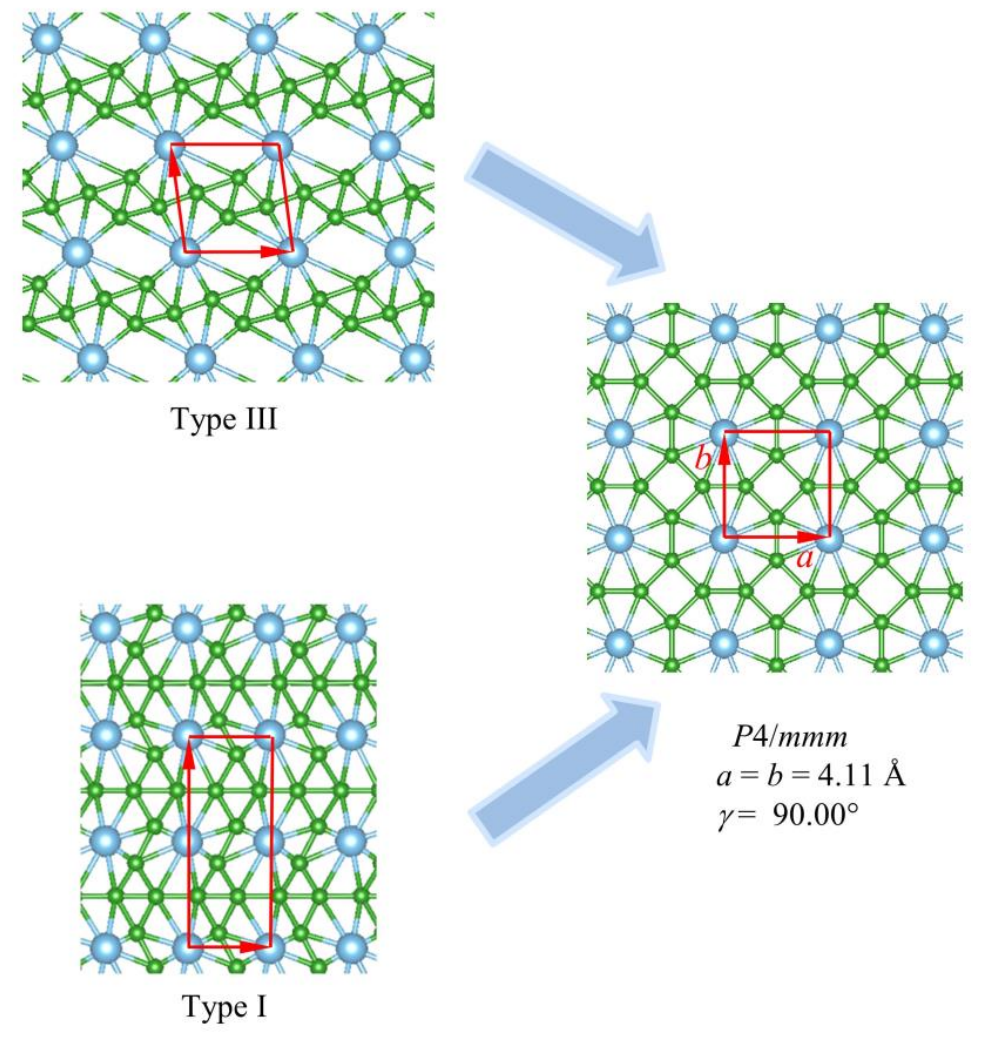
\includegraphics[width=0.86\textwidth]{figs/ch5_cell_change.png}
  \centering
  \caption{分别从\rom{1}型和\rom{3}型的初始构型演变为最后稳定的\ce{TiB4}结构}
  \label{fig:ch5_cell_change}
\end{figure}

\section{单层TiBn的结构多样性与稳定性}
在绪论部分已经介绍了以过渡金属为中心的多配位硼轮平面团簇能够表现出很好的结构稳定性,同时结合了已经有理论预测报道的由过渡金属和硼所构成的稳定二维平面结构。我们因此认为过渡金属和硼能够形成种类多样且拥有新颖优异的物理化学的二维材料。在本论文的工作中,我们选择四周期第一系过渡金属钛作为嵌入硼平面的金属原子,探索其可能出现的稳定平面构型。

在该章所描述的工作之前,有如下一些文献预测报道了钛硼二维材料。2014年由Zhang等预测报道的单层\ce{TiB2}结构\cite{zhang2014prediction},结构上,钛原子由六个硼原子包围,硼原子形成蜂窝状结构,该结构在能带结构中存在狄拉克锥,最大费米速度为0.57×106m/s,约为石墨烯的一半。2017年由Qu等所报道的单层平面\ce{TiB4}结构\cite{qu2017two},钛原子由八个硼原子包围组成八配位的钛硼结构,八个硼原子到中心钛原子的距离均相等,且从侧视图可以看到,整个结构是一个完美的平面,原子之间没有起伏。2017年Wang\cite{wang2017semimetallic}等报道了多种二维钛硼平面构型,构型中的钛硼原子数比从$1:2$到$1:16$,这一系列的构型可分为两大类,一类为钛硼所组成的单层平面结构,一类为钛原子处在两层硼平面之间的三明治结构,其中的\ce{TiB12}的能带结构中存在狄拉克锥,且通过对结构施加横向张力,结构的功函数和电导能够被调控。

需要强调的是,所有已经报道的钛硼二维结构都是通过材料搜索的方法发现的。材料搜索的方法尤其一定优势,它只需要极少的起始变量就能对特定化学配比的化合物在势能面上以很高的自由度进行材料搜索。但也因为自由度过高,搜索过程中所可能经历的构型数量非常巨大,而其中的一些初始结构往往会优化为相同的构型,这在一定程度上即浪费时间,也浪费了计算资源。另外,固定元素之间形成化合物往往会存在特定的结构特征,利用结构特征将能够确定合理的初始构型集合,从而大大减少计算过程中所需要的时间,减少计算资源的浪费。以二维钛硼结构为例,我们可以发现,稳定的钛硼构型都是由钛为中心,硼环绕的超多配位结构,这也符合硼与过渡金属形成多配位团簇时出现的结构稳定性。

以此为出发点,我们将所要探索的二维钛硼结构的集合限制在钛硼单层,并且钛作为中心原子被硼原子环绕。利用这样的初始结构,我们优化得到了全部已经报道的钛硼单层二维结构,并发现了一些新的具有新颖性质的稳定结构。我们的计算覆盖了很大的化学配比范围,并基本能够确保包含了所有可能的结构组合。同时,所需要计算的构型数量也并不很大,通过与高通量工作流工具结合,能够很快完成结构的优化和性质的计算。

硼原子构成硼平面的结构多样性丰富,但结构的区别均体现在空位分布位置的不同上,也就是说,硼原子网络始终保持为三角格子。过渡金属硼构成的单层平面结构,过渡金属均采取多配位的结构,同时硼网络均能够看做是三角各自轻微程度扭转而成的,如图\ref{fig:ch5_cell_change}所示,我们展示了如何从初始构型通过胞和原子的轻微位置变化获得新的稳定结构。利用这样的结构上的特征,我们选择在硼原子构成的三角格子网络中用过渡金属原子嵌入网络并替换一个或多个硼原子来构造初始平面单层钛硼网络。这样在结构优化过程中,原子仅仅在原始位置周围移动调整网络的空间结构,即保证能够在势能面的每个可能局域极小值附近都有初始构型,从而对势能面上的所有局域极小结构进行遍历,并考察结构稳定性。

下面小结将详细描述初始结构的生成过程,与其结构稳定性的考察过程。

\subsection{结构多样性与结构的生成}

对应方法后部分之前文献报道的二维\ce{TiB2}化合物为三明治夹层结构,硼原子形成两层硼平面,钛原子在两层硼平面中间作为插层并与周围的硼原子成键,其中钛原子与硼原子之间的距离为\num{1.19}\si{anstrom}。类似的过渡金属-硼构成的三明治夹层结构在其他的钛硼、铁硼二维结构中也由发现。而我们的工作,旨在探究钛原子与硼形成单层的钛硼平面,并对比所有这类单层平面的结构稳定性。为得到这样的单层过渡金属硼平面,我们按照如下的方法来构建初始构型。首先,确保硼原子按照三角格子密堆的形式形成硼单层网络,其次,在网络中插入过渡金属钛原子与硼成键。
然而,由于过渡金属的半径较硼的大的多,其原子很难只是通过替换单个硼原子与硼原子网络中的其余硼原子通过六配位的方式来嵌入硼原子网络中而形成二维钛-硼单层结构。根据过渡金属与硼形成轮状团簇时实验观测到的都是多配位的团簇这一结论,我们认为,在单层过渡金属-硼平面中,过渡金属同样应该倾向于与硼原子形成大于六的高配位。因此,综上两个原则,我们选择初始结构应为在三角硼平面网格的基础上,通过过渡金属替换多于一个的相邻的硼原子来构建结构。所构建的一系列初始构型的多样性可以从以下两点体现:1)可以将硼原子构成的网格以不同的胞进行划分,这里不等价胞的选取我们用到了第四章所介绍的算法,并在我们自己编写的代码上实现。2)相邻的多个硼原子可以有多种聚集方式,而且可以出现在给定单胞的不同的位置。但由于晶格的对称性,所生成的许多结构事实上是互相等价的,在这里等价结构的查重我们用到了第四章中的固定胞不同结构的查重算法,同样在我们自己编写的软件中实现。下面将针对钛硼单层的初始结构,简要描述这两类体现多样性的查重算法是如何实现的。

\begin{figure}
  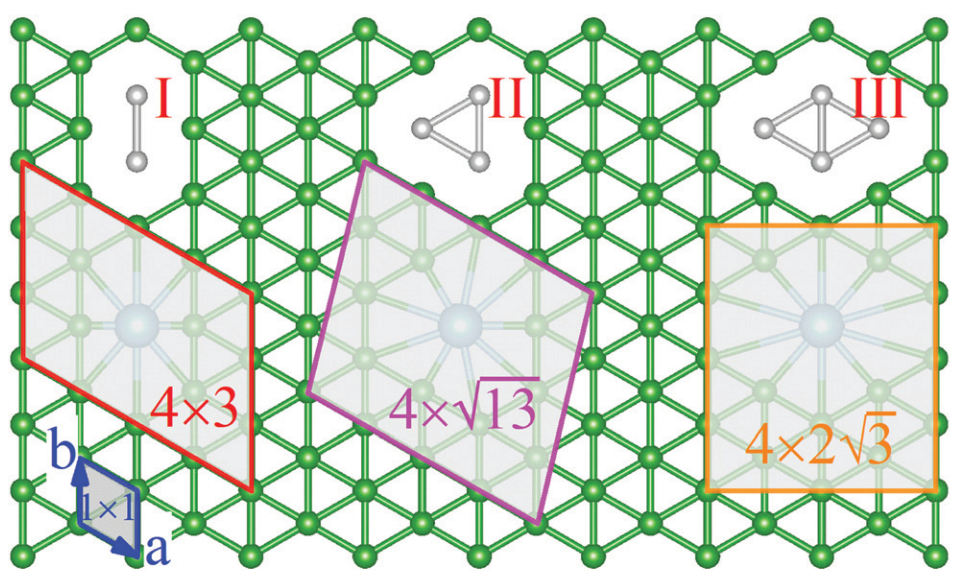
\includegraphics[width=0.92\textwidth]{figs/ch5_how_cell_choose.png}
  \centering
  \caption{单层硼化钛的结构生成示意图。在\rom{1}型、\rom{2}型和\rom{3}型中,一个钛原子分别替代两个、三个和四个硼原子。蓝线勾勒出的菱形表示二维三角晶格的单元格。还同时显示了超胞。大的天蓝色球和小的绿色球分别代表钛原子和硼原子。灰色的球代表要被取代的硼原子。}
  \label{fig:ch5_how_cell_choose}
\end{figure}

首先,我们通过对硼平面的原胞(图\ref{fig:ch5_how_cell_choose}中左下角的深蓝色$1\times 1$晶胞)按不同方式进行展开,得到更大的硼三角超晶格单胞。我们使用厄米标准型矩阵(HNF)\cite{hart2008algorithm}来展开不重复的超胞。这里,我们限定所要考察的结构的尺寸,最大不超过\num{16}倍的原胞面积,即厄米标准型矩阵的行列式的值最大不超过\num{16},因为原胞中仅有一个硼原子,所以其行列式的值也是元胞中的硼原子数量,我们最大得到的硼原子超胞就包含\num{16}六个硼原子。每种厄米矩阵对应一种超胞形式,不同的厄米矩阵可以有相等的行列式值,相同的行列式的厄米矩阵代表原子数相同但超胞不等价的两种超胞构型。图\ref{fig:ch5_how_cell_choose}展示了三种不同面积的超胞。在获取固定的超胞后,我们对硼原子进行替换,用一个过渡金属原子一次性替换两个三个或四个硼原子,将过渡金属放在所替换的硼原子的空位的中心。
如图\ref{fig:ch5_how_cell_choose}所示阴影部分中的替代,共有三种方式,分别对应替换两个,三个和四个硼原子,分别形成过渡金属与相邻硼原子配位数为八,九和十的三种结构形式,我们将其初始结构分别命名为\rom{1}型\rom{2}型和\rom{3}型初始构型。替换后的构型会存在等价的构型,我们通过查重算法将等价的构型去除。同时需要提到的是,根据已知经验,过渡金属应该与硼形成配位,而金属-金属直接相连的结构能量上并不占优,为验证这个条件,我们在其中一个超胞下面的构型中,测试了几个金属金属相连的生成构型,结果显示与相同化学计量的构型相比,其能量高出许多。

最后,通过以上步骤,我们一共获得了胞面积小于等于16的超胞下取代后的构型,\rom{1}型\num{210}个,\rom{2}型\num{98}个,\rom{3}型\num{150}个。这样的数量与全局搜索算法所需要的总数相比少了许多(全局搜索算法对特定原子数配比,需要进行上千个结构的优化计算)。值得关注的是,我们使用较少的计算量就能够发现全局搜索所能发现的全部单层稳定构型,并还发现了能量比其更低的构型,这个结果我们将在下一节详细叙述。这种搜索策略高效的原因,是因为我们在初始结构的生成中较好的应用了已知的结构上的样式特征,即硼三角网格的过渡金属硼形成多配位。加入先验知识而加快搜索的效率是该方法的一个主要优势,

\begin{figure}
  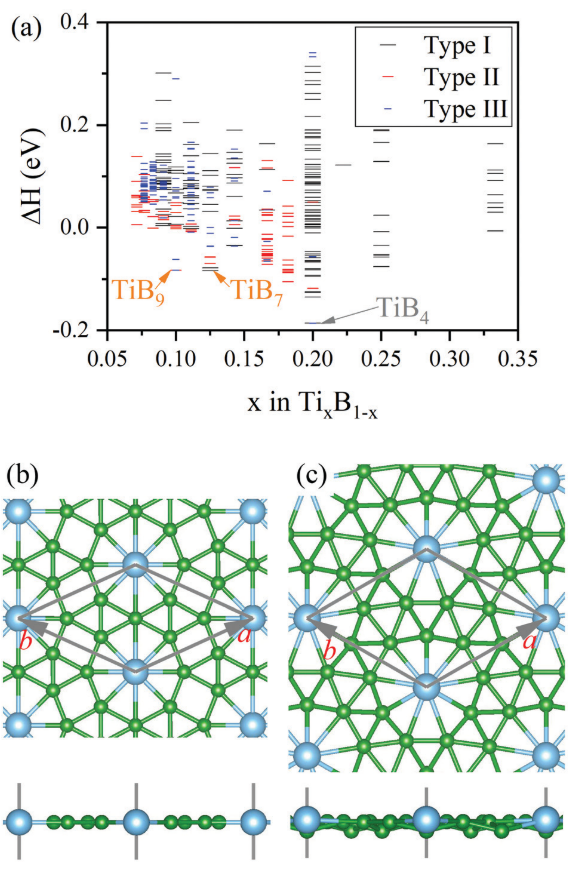
\includegraphics[width=0.72\textwidth]{figs/ch5_energy_hull.png}
  \centering
  \caption{(a)单层硼化钛的形成焓随钛浓度的变化。预测的(b) \ce{TiB7}和(c) \ce{TiB9}的原子结构的俯视图和侧视图。}
  \label{fig:ch5_energy_hull}
\end{figure}

定性讨论单与稳定结构的电子结构层基于对上面提到的生成的钛硼原子比例从$1:2$到$1:13$的各种钛硼单层构型,我们进行了能量和电子结构的高通量计算,并对每种钛硼原子比例下能量较低的构型分析了其超导性质。

由于钛硼的硼硼键长之间存在巨大的差别,我们认为钛硼不容易出现六配位的结构,在过往报道的文献中,\ce{TiB4}单层是一个全平的平面,其中钛和硼形成八配位的等边多边形,以及硼硼之间形成的四边形,如图\ref{fig:ch5_cell_change}右边的结构优化后的\ce{TiB4}所示。因此我们认为该结构是有一个钛原子处于中心的\ce{TiB8}轮状团簇图案平铺而成的。

上一节所述,如图\ref{fig:ch5_how_cell_choose}所示,我们在硼三角网格平面引入多空位(\rom{1}型,\rom{2}型和\rom{3}型分别代表替换两个三个和四个相互连接的硼原子),并在大空位中心放入过渡金属钛原子形成八元九元和十元环的钛硼结构。并基于HNF矩阵和结构识别,我们生成了钛硼单层结构的初始构型并对他们进行了结构优化和能量的计算。为了描述钛硼单层的的稳定性和钛原子在结构中占比的关系,我们定义下列形式的单层构型形成能:
\begin{equation}
  \Delta H = E_{Ti_xB_{1-x}} - xE_{Ti} - (1-x)E_{B},
\end{equation}
其中$E_{Ti_xB_{1-x}}$,$E_{Ti}$和$E_B$分别是构型单胞的总能量,钛原子在其稳定的六方密堆体相结构中的原子能量,以及单个硼原子在硼平面中的能量。

图\ref{fig:ch5_energy_hull}(a)展示了各个\ce{Ti_xB_{1-x}}构型的形成能$\Delta H$随着钛原子在结构中占比的变化。值得注意的是,其中\ce{TiB4},即已经被报道的平面钛硼单层结构有着最低的形成能,该构型可以分别由如图\ref{fig:ch5_how_cell_choose}左边两个分别属于\rom{1}型和\rom{3}型的初始结构得到。在钛的比例大于\num{0.2}时,初始结构主要是\rom{3}型,因为此时需要在超胞中去除更多的硼原子来放入一个钛原子。而区要代替较少的硼原子的\rom{1}型和\rom{2}型结构则更多的是钛比例较少的构型。

在钛硼比为$1:7$的\ce{TiB7}结构中,形成能最低的结构如图\ref{fig:ch5_how_cell_choose}(b)所示,它是一个全平的平面,优化后该结构的晶格参数为:$a=b=5.72\AA,\gamma=130.94^{\circ}$,该结构空间群为$Cmmm$。该结构中,钛原子与硼原子组成八元环,其中的钛硼键的长度分别为\num{2.15}\si{anstrom},\num{2.18}\si{anstrom}和\num{2.37}\si{anstrom}。结构中硼原子之间还组成了三元环与四元环(此处硼硼原子成键的标准选择为化合物中出现的最大的硼-硼原子键作为上限,超过该长度则认为硼硼原子不成键),因此该结构可以认为是由\ce{TiB8}轮状碎片与三元四元硼碎片平铺拼接而成的。
我们同样在图\ref{fig:ch5_tib7_last3}中展示了该钛原子浓度下能量最低的三种构型,以及能够优化到这些结构的初始构型,可以看到,初始结构和最终结构的原子位置只是发生了很小的变动,说明了我们生成的初始构型的方式是合理的。其中能量次低的构型为$P2/m$空间群,每个原子的平均形成能与最稳定构型相差了6meV,这个不大的能量差别说明我们方法对特定构型势能空间局域极小值的判断精度达到了<10meV的级别,能够区别搜索能量相差不是很大的构型。这个能量次低的构型与最低的构型非常相似,区别是该构型的a,b晶格参数不相等,是之前文献使用全局搜索软件USPEX得到的该配比下的最稳定构型。能量第三低的结构为$Pm$空间群,能量比次低结构高出了14meV。

\begin{figure}
  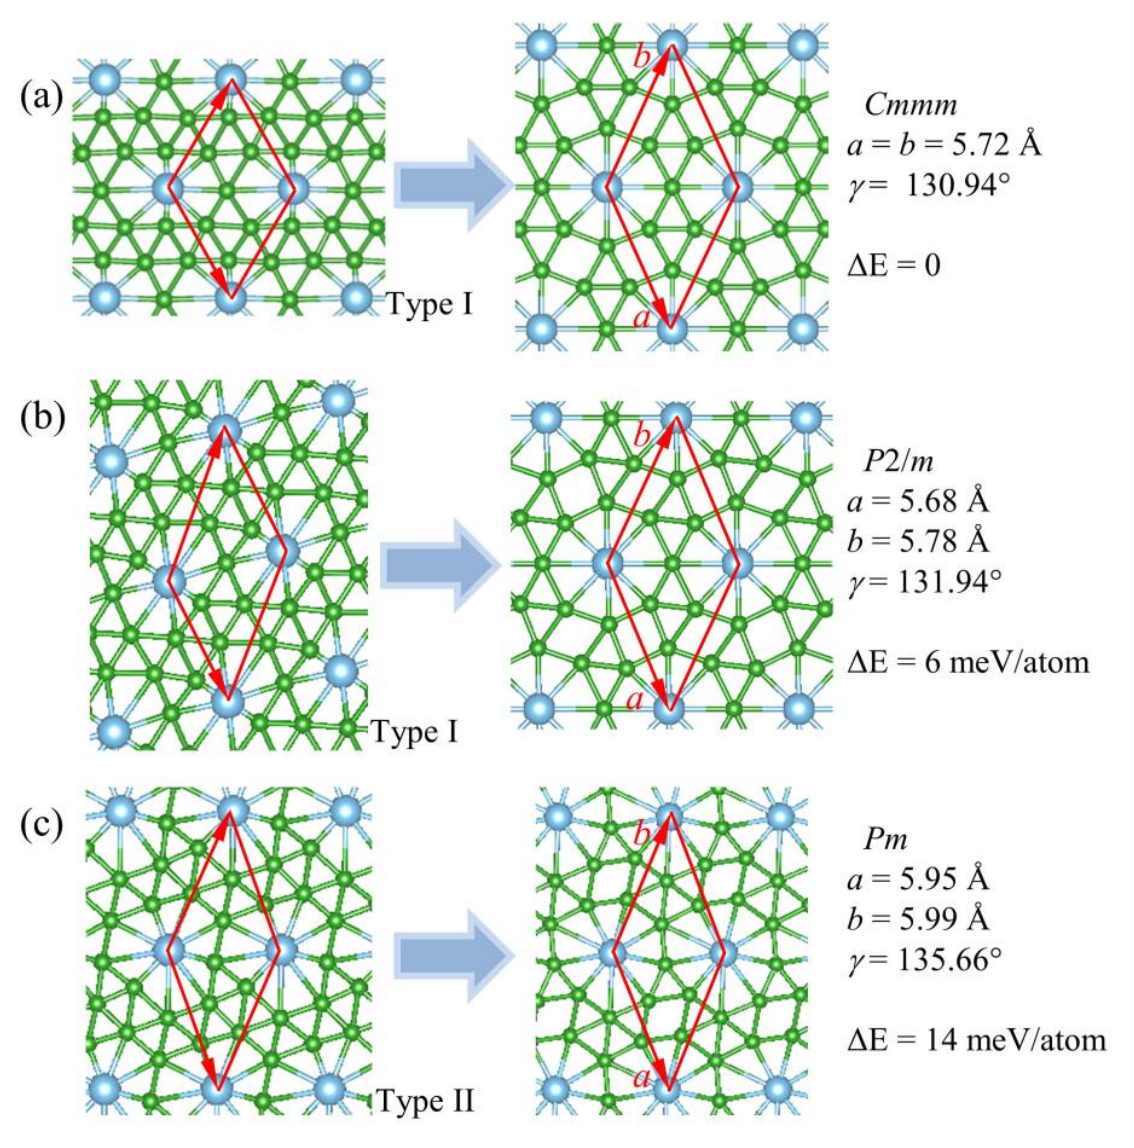
\includegraphics[width=0.72\textwidth]{figs/ch5_tib7_last3.png}
  \centering
  \caption{\ce{TiB7}能量最低的三种构型,以及它们的初始构型。}
  \label{fig:ch5_tib7_last3}
\end{figure}

我们还着重考察了钛硼比例为$1:9$的构型,其能量最低的构型如图\ref{fig:ch5_energy_hull}(b)所示,晶格参数为$a=b=5.83\AA,\gamma=120^{\circ}$,空间群为$P31m$。结构中由两种不等价(不同维科夫位点)的硼原子,每个钛原子被九个硼原子所包围,钛硼键的键长分别为2.22A和2.43A。硼原子形成三元环并和钛-硼构成的九元轮状碎片相连接。能量最低的构型可以对应由如图\ref{fig:ch5_tib9}所示的\rom{2}型\rom{3}型两种初始构型优化而来。这个稳定的构型已经被之前的文献报道,这再次说明了我们所采用的搜索算法的可靠性。

\begin{figure}
  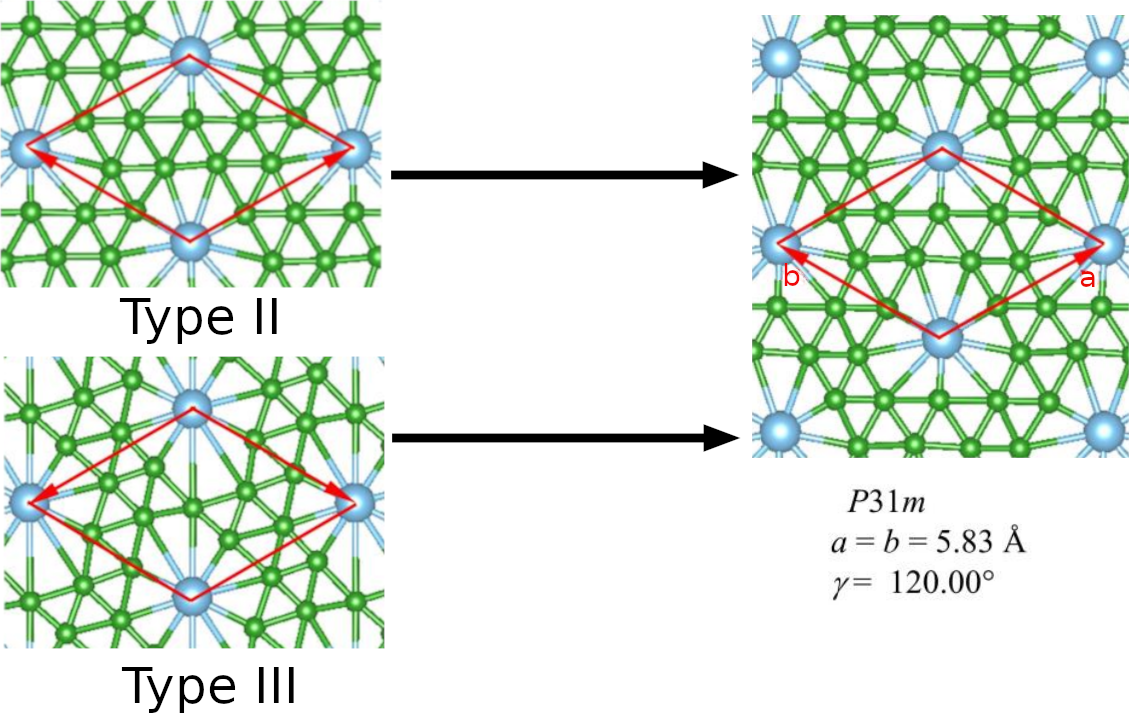
\includegraphics[width=0.82\textwidth]{figs/ch5_tib9.png}
  \centering
  \caption{\ce{TiB9}能量最低的构型,以及初始构型}
  \label{fig:ch5_tib9}
\end{figure}

该研究所涉及的初始结构的钛硼原子比例共\num{14}种,除了上面详细描述的\ce{TiB7}和\ce{TiB9}两种结构,其它浓度下能量最低的构型分别展示在图\ref{fig:ch5_all_configs}中。我们可以发现,钛的浓度过高或过低都不利于结构的稳定,当钛在结构中占比过高时,钛原子倾向于聚集形成团簇,并和硼原子构成的团簇分离。当钛原子浓度过低时,钛原子的表现为扭曲了硼的平面稳定结构,并且,由于我们没有考虑钛原子和空位同时出现的情况,硼的无空位三角网络并不稳定,因此同样难以获得稳定的结构。另外在这些结构中能发现另一有趣的现象,其中\ce{TiB4},\ce{TiB7},\ce{Ti2B9}以及\ce{TiB5}这几个各自浓度下能量最低的构型形成了全平的完美的二维结构,说明这些浓度下电子在平面上很好的分布。我们尚不知道这种全平的完美二维单层是否由特殊的性质,但为结构的多样性以及结构的研究提供了很好的素材。

我们分析了\ce{TiB7}和\ce{TiB9}两个单层平面能带,态密度和投影态密度等电子结构性质如图。\ce{TiB7}和\ce{TiB9}均为金属,费米能级穿过其能带。\ce{TiB7}单层费米能级附近的态主要是由钛的d轨道和硼的p轨道构成的,而在\ce{TiB9}中,费米能级附近的波函数主要来自于钛的d轨道。与\ce{TiB4}单层相比,$d$轨道能级在单层中构成了一个接近水平的能带,这个轨道大大增加了费米能级附近的态密度,因此可能使其成为潜在的超导材料。

\begin{figure}
  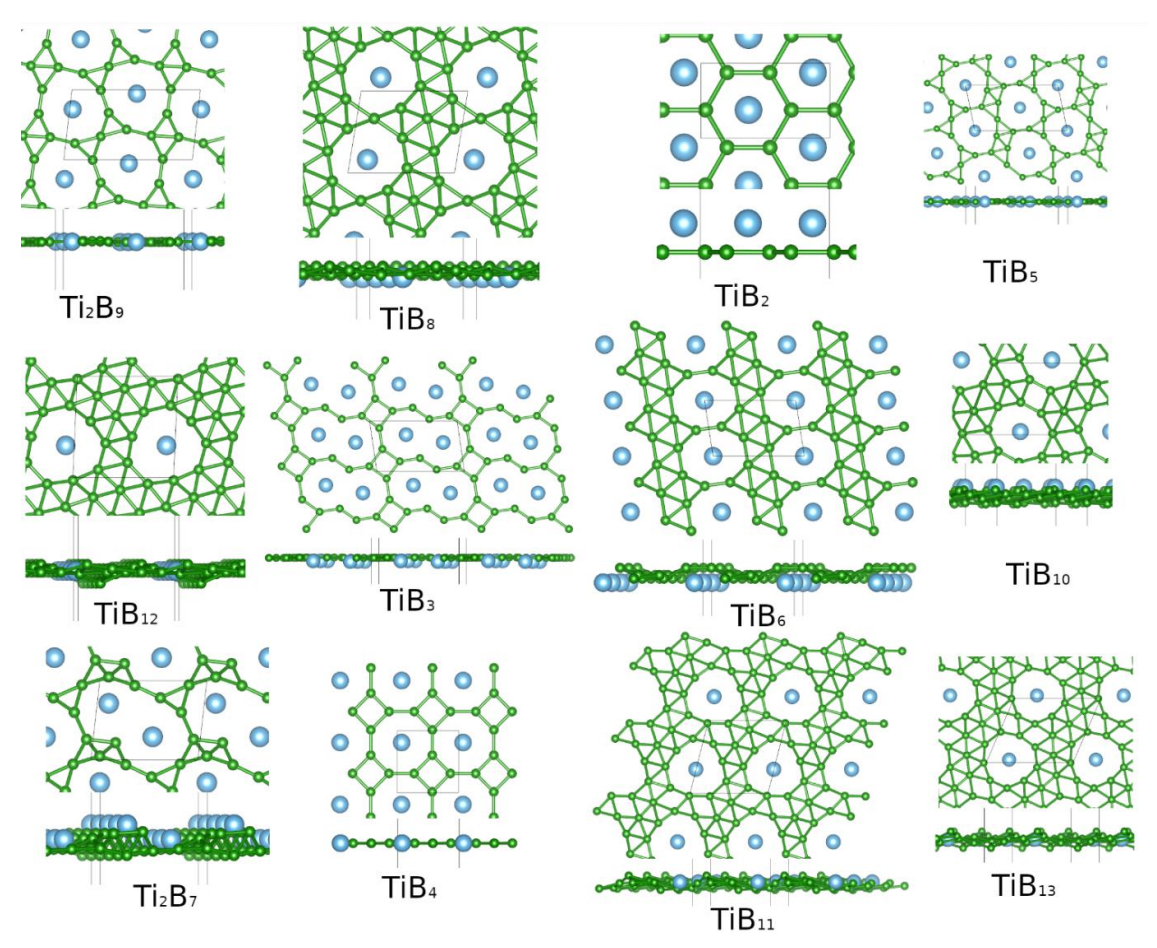
\includegraphics[width=0.96\textwidth]{figs/ch5_all_configs.png}
  \centering
  \caption{钛硼单层在所有我们探索的浓度下能量最低的构型,图片展示了结构的俯视图和侧视图。}
  \label{fig:ch5_all_configs}
\end{figure}

\section{钛硼二维材料的超导性质}
为探究潜在的超导性质,我们分析了\ce{TiB7},\ce{TiB9}单层和\ce{TiB7}双层的电声耦合性质。。根据第三章中的叙述,定义的由Eliashberg谱得到的无量纲的电声耦合常数$\lambda$有以下形式:

\begin{equation}\label{eq:lambda_coupling}
  \lambda = 2 \int d\omega \frac{\alpha^2 F(\omega)}{\omega}.
\end{equation}
其中$\alpha^2 F(\omega)$是Eliashaberg谱函数,可以通过下列形式计算得到,代入以上方程得到等式:

\begin{equation}\label{eq:elishaberg_calc}
  \alpha^2 F(\omega) = \frac{1}{2\pi N(\epsilon_F)}\frac{1}{N_{\bm{q}}}
  \sum_{\bm{q}j} \frac{\gamma_{\bm{q}j}}{\omega_{\bm{q}j}}
  \delta(\omega-\omega_{\bm{q}j}),
\end{equation}
表达式中$N(\epsilon_F)$是费米能级处的电子密度,公式中的狄拉克$\delta$函数在实际计算中可以用高斯函数近似。$\omega_{\bm{q}j}$和$\gamma_{\bm{q}j}$分别是模为$j$的声子在波矢$\bm{q}$处的频率和线宽。最后表达式中的$N_{\bm{q}}$是第一布里渊区所统计的波矢数量,在实际计算中,为了得到准确的结果,我们往往需要很密的$\bm{q}$点的划分。式中给定波矢和特定声子振动模式下的电声耦合系数为:

\begin{equation}
  \lambda_{\bm{q}j} =
  \frac{\gamma_{\bm{q}j}}{\pi \hbar N(\epsilon_F) \omega^2_{\bm{q}j}},
\end{equation}
使用该等式,体系的各向同性耦合常数$\lambda$可写为以下形式:
\begin{equation}\label{eq:lambda_from_phonon}
  \lambda = \frac{1}{N_{\bm{q}}}\sum_{\bm{q}j} \lambda_{\bm{q}j}.
\end{equation}
从声子谱中计算得到每个振动模式不同频率下的耦合系数后代入上式(\ref{eq:lambda_from_phonon})就能得到无量纲的材料的电声耦合常数。

\begin{figure}
  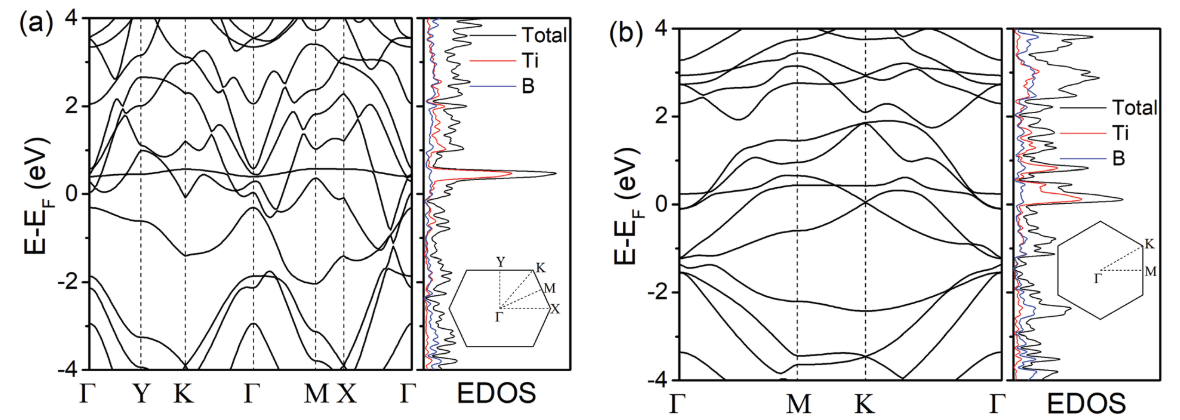
\includegraphics[width=0.96\textwidth]{figs/ch5_bands.png}
  \centering
  \caption{\ce(TiB7)和\ce{TiB9}的能带和态密度。}
  \label{fig:ch5_bands}
\end{figure}

\subsection{单层TiB7的超导性质}
图\ref{fig:ch5_tib7_sc_all}展示了TiB7单层的声子谱及各个振动模式不同频率的声子线宽$\gamma_{\bm{q}j}$,Eliashhberg函数$\alpha^2 F(\omega)$和$\lambda(\omega)$($\omega$为计算的声子的频率上限)。首先可以确定的是,从图\ref{fig:ch5_tib7_sc_all}(a)的\ce{TiB7}声子谱可以看出,声子谱中没有虚频说明结构可以在单层状态稳定存在。从图中可以看出,主要是低频(<400cm-1)的振动模式贡献了电声耦合。
从Eliashberg函数$\alpha^2 F(\omega)$可看出,在频率为约200cm-1处有数个尖峰,其主要是由该频率位于$\Gamma$点周围的声子贡献的,此处在$\Gamma$点的声子线宽较大。我们将$\Gamma$点附近频率从160到240cm-1处的声子谱放大在图\ref{fig:ch5_tib7_sc_all}中展示,此处有四种振动模式$\omega_1$,$\omega_2$,$\omega_3$和$\omega_4$,分别代表了如图\ref{fig:ch5_tib7_sc_all}(b)所示的四种振动。
其中,$\omega_1$为面内的剪切模(图\ref{fig:ch5_tib7_sc_all}(c)),它的振动模式的对称性为$C_3$。图\ref{fig:ch5_tib7_sc_all}(d)(e)(f)为其余三个垂直于面平面的振动模式,通常在文献中,将这种垂直于面的振动模式称为呼吸模。在四种模式中,剪切模$\omega_1$和呼吸模$\omega_3$、$\omega_4$的声子线宽较大。$\omega_2$处的声子线宽较小,但由于其该带很平,在态密度中这一频率处贡献很大。综上两个因素导致了在200cm附近Eliashberg函数的绝对值较大,贡献了很大的电声耦合。
根据McMillan–Allen–Dynes参数化Eliashberg方程,我们可以估计超导临界温度$T_c$:
\begin{equation}
  T_c = \frac{\omega_{\mathrm{log}}}{1.2}
  \exp{\left[ {-\frac{1.04(1+\lambda)}{\lambda-\mu^*(1+0.62\lambda)}} \right]}
\end{equation}
其中$\omega_{\mathrm{log}}$为Eliashberg函数在全频率范围的对数平均,表示如下:
\begin{equation}
  \omega_\mathrm{log} = \exp \left[ {\int d\omega \log(\omega)W(\omega)} \right],
\end{equation}
其中的权重$W$定义为:
\begin{equation}
  W(\omega) = \frac{2}{\omega} \frac{\alpha^2 F(\omega)}{\omega}.
\end{equation}

\begin{figure}
  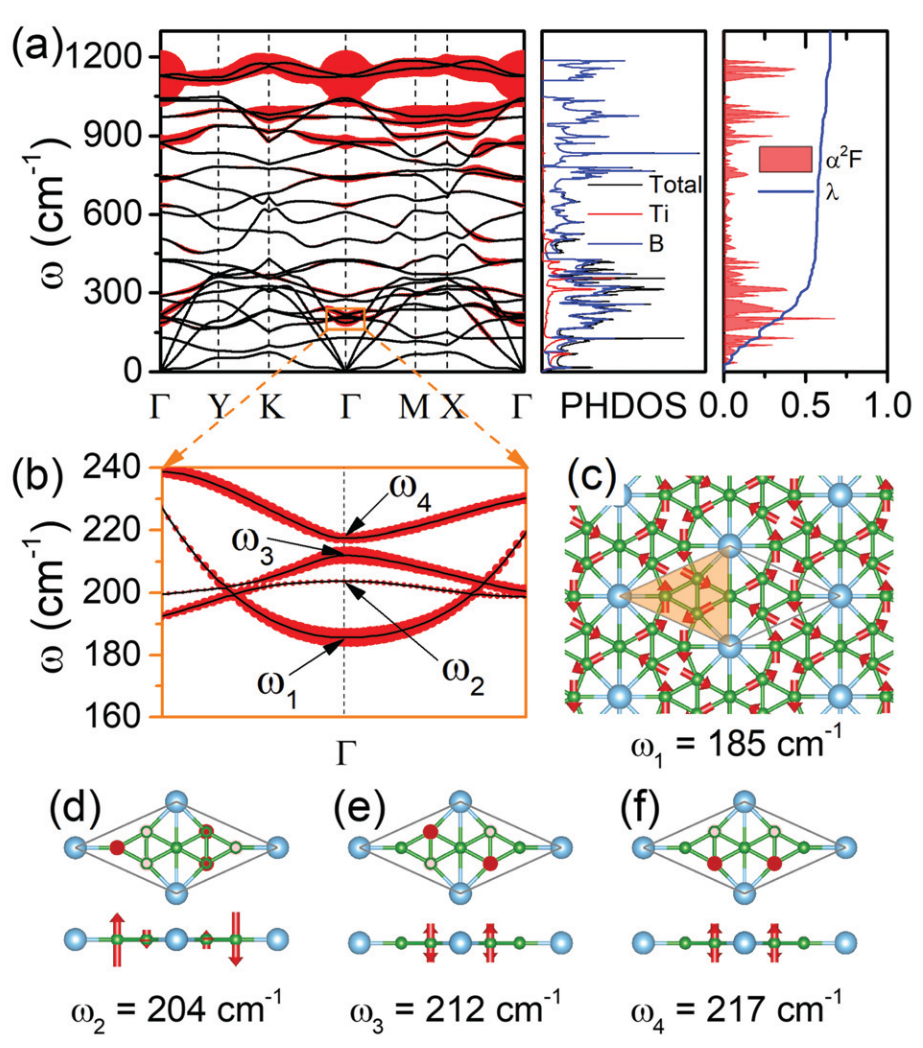
\includegraphics[width=0.96\textwidth]{figs/ch5_tib7_sc_all.png}
  \centering
  \caption{(a)红色包围的区域中声子色散与声子线宽$\gamma_{qj}$、声子态密度以及单层\ce{TiB7}的Eliashberg函数$\alpha^2 F(\omega)$和$\lambda(\omega)$($\omega$。(d-f)层的呼吸模。红色箭头及其长度代表了相应振动模式的方向和振幅。}
  \label{fig:ch5_tib7_sc_all}
\end{figure}

根据之前关于硼材料研究的文献\cite{penev2016can,zhao2016superconductivity,zhao2018multigap,liao2017phonon,yan2020superconductivity},
上面经验公式中的库伦排斥势$\mu^*$我们选取了$\mu^*=0.1$来计算超导转变温度。图\ref{fig:ch5_tib7_coupling}中展示了电声耦合系数$\lambda$在倒空间中的变化情况,我们可以看到,在$\Gamma$点附近是一个以$\Gamma$点为中心的哑铃形状的分布,其最大的$\lambda_{\bm{q}j}$值大于\num{1.0}。全部倒空间中的电声耦合系数除了$Y$对称点处均大于\num{0.6}。因而总的电声耦合常数$\lambda$为\num{0.65}。
将$\lambda$代入以上公式中我们得到单层\ce{TiB7}平面的超导转变温度为\num{8.3}K。该超导温度高于报道的锂沉积石墨烯的超导转变温度,即理论计算的超导温度为$T_c=8.1K$\cite{profeta2012phonon},实验测量得到的超导转变温度为\num{5.9}K\cite{ludbrook2015evidence}。
在钛硼化合物中,原子质量较小的硼元素是常规BCS超导电声耦合的主要原因。同样的所有的单层金属硼平面均显示出超导性质,而超导转变温度和硼平面的空位浓度之间存在先减少后增加的关系。当空位浓度为\num{1/9}时,最稳定的alpha硼平面的超导转变温度为3.7K。当空位浓度增加到1/8时超导转变温度提高到5.8K。我们可以看到,通过引入钛原子增加里材料的电声耦合并提高了超导转变温度$T_c$。钛单质块体中测量得到的超导转变温度最大为0.38K[],因此在TiB7中超导主要是由硼元素所贡献的。

\begin{figure}
  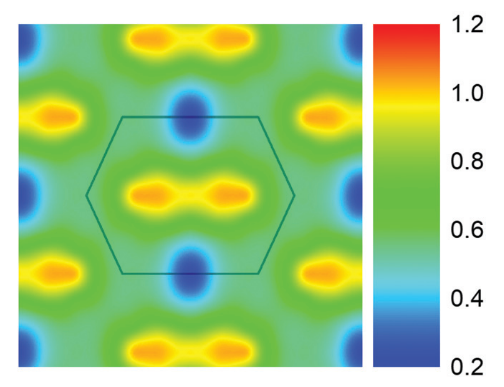
\includegraphics[width=0.72\textwidth]{figs/ch5_tib7_coupling.png}
  \centering
  \caption{电声耦合系数$\lambda_{q}$在倒空间中的变化情况}
  \label{fig:ch5_tib7_coupling}
\end{figure}

二维BCS型超导体\ce{AlB6}中报道了通过拉伸材料可以提高,\SI{12}{\percent}的拉伸应变可以将超导温度提高到30K。我们同样对\ce{TiB7}平面作了相似的拉伸应变,从图\ref{fig:ch5_tib7_strain}中可以看到,拉伸并没有提高超导温度,在世家5\%的拉伸应变后材料的超导转变温度降低到了约2K。尽管随着应力的增加$\omega_\mathrm{log}$持续增加,但是总的电声耦合常数和超导转变温度均减小。其中,$\Gamma$点处低频的声子频率随应力增加而增加,高频的声子频率岁应力的增加而减少。图\ref{fig:ch5_tib7_strain}中展示了高频声子和低频声子频率随拉伸应变的变化关系。我们还在图?中展示了声子谱以及Eliashberg函数随应力变化的详细关系。若拉伸应变会减小超导转变温度,则相反的压缩应变应该增加超导转变温度,如\ce{B5}硼平面\cite{cheng2017suppressed},二维\ce{TiS2}\cite{liao2020doping},
甚至并非属于BCS超导的\ce{FeS}层状结构\cite{nie2009suppression}。然而,对于\ce{TiB7}单层压缩应变在达到1\%后结构声子谱中就出现了如图?中的严重的虚频,我们认为该强度的应变就会使结构出现相变而丧失超导性质。

\begin{figure}
  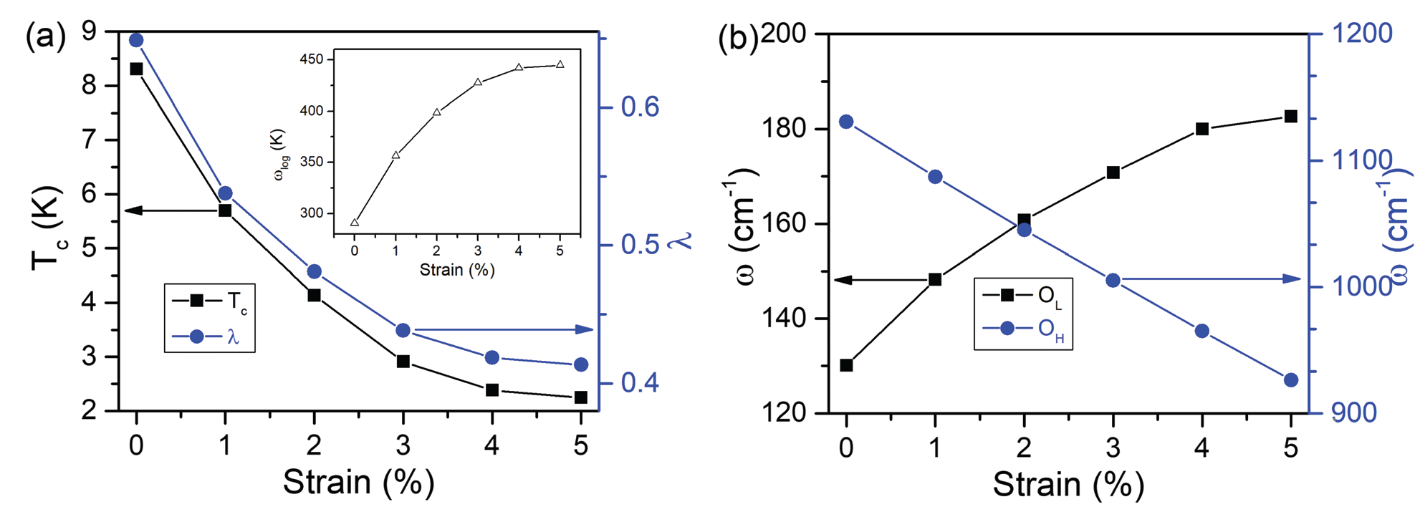
\includegraphics[width=0.96\textwidth]{figs/ch5_tib7_strain.png}
  \centering
  \caption{计算了\ce{TiB7}单层的$T_c$和电声耦合常数$\lambda$随等双轴拉伸应变的变化。以及对数平均声子频率($\omega_{\mathrm{log}}$)的变化。(b)在$\Gamma$处的光学声子的最低($O_L$)和最高($O_H$)频率随应变变化的函数。}
  \label{fig:ch5_tib7_strain}
\end{figure}

\begin{figure}
  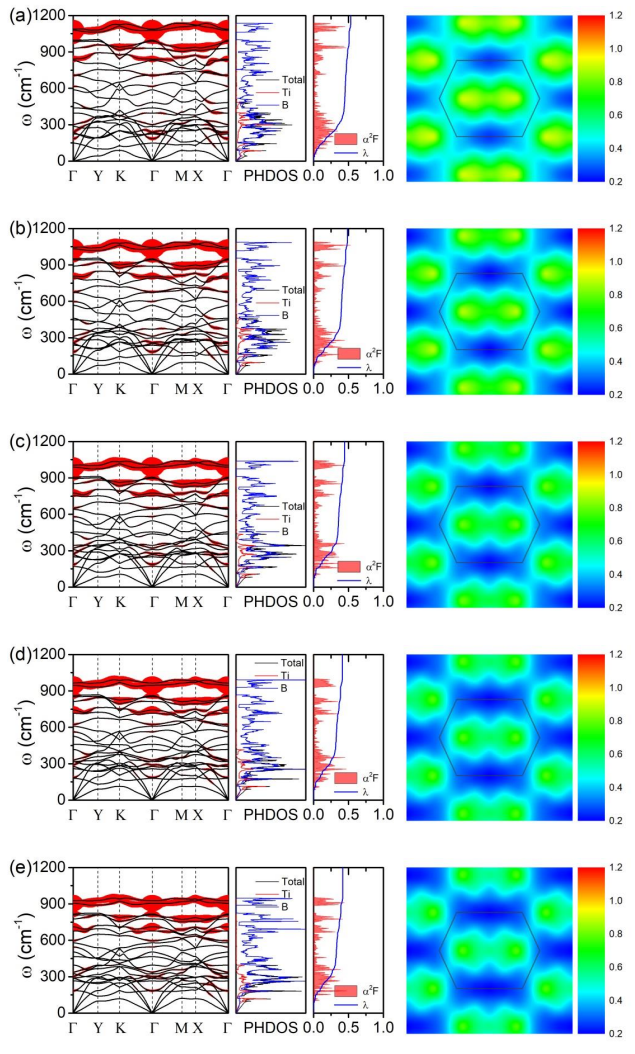
\includegraphics[width=0.88\textwidth]{figs/ch5_details_strains.png}
  \centering
  \caption{在拉伸应变为(a) 1\%, (b) 2\%, (c) 3\%, (d) 4\%, (e) 5\%时,\ce{TiB7}单层薄膜的声子色散以声子线宽$\gamma_{qj}$、声子态密度、Eliashberg函数$\alpha^2 F(\omega)$和$\lambda(\omega)$和耦合常数强度在倒空间的分布。}
  \label{fig:ch5_details_strains}
\end{figure}

作为对比我们还理论计算了\ce{TiB9}单层的超导相关性质。如图\ref{fig:ch5_tib9_phonon},该结构声子谱中同样不存在虚频说明其能够以二维的形式稳定存在。电声耦合的计算结果如图\ref{fig:ch5_tib9_phonon}所示,其各向同性平均电声耦合系数$\lambda$为0.40.在$\Gamma$点附近其电声耦合系数最大为$\lambda_{\bm{q}j}$约为0.7.由此可以估计其超导转变温度为1.2K。如前面描述的,\ce{TiB7}单层是完全平面的结构,而\ce{TiB9}不同其垂直方向有原子的起伏。为了研究垂直方向的起伏对超导性质的影响,我们构造了完全平整的\ce{TiB9}构型作为对比,并研究了其声子部分振动模式信息的变化作为参照,以确定是否完全平整的平面能够提高电声耦合从而提高超导性质。
优化后的\ce{TiB9}平面构型的晶格参数增加了1.2\%,且总能上升了0.19eV。然而,计算结果显示该构型有明显的虚频如图\ref{fig:ch5_tib9_phonon_a}所示,因此无法进一步研究电声耦合性质以作为对比。

\begin{figure}
  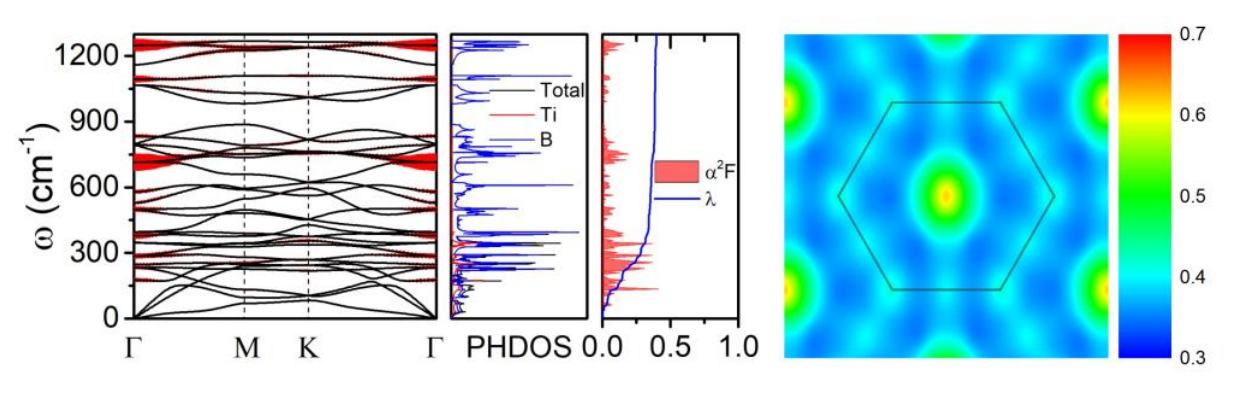
\includegraphics[width=0.96\textwidth]{figs/ch5_tib9_phonon.png}
  \centering
  \caption{\ce{TiB9}单层薄膜的声子色散以声子线宽$\gamma_{qj}$、声子态密度、Eliashberg函数$\alpha^2 F(\omega)$和$\lambda(\omega)$和耦合常数强度在倒空间的分布。}
  \label{fig:ch5_tib9_phonon}
\end{figure}

\begin{figure}
  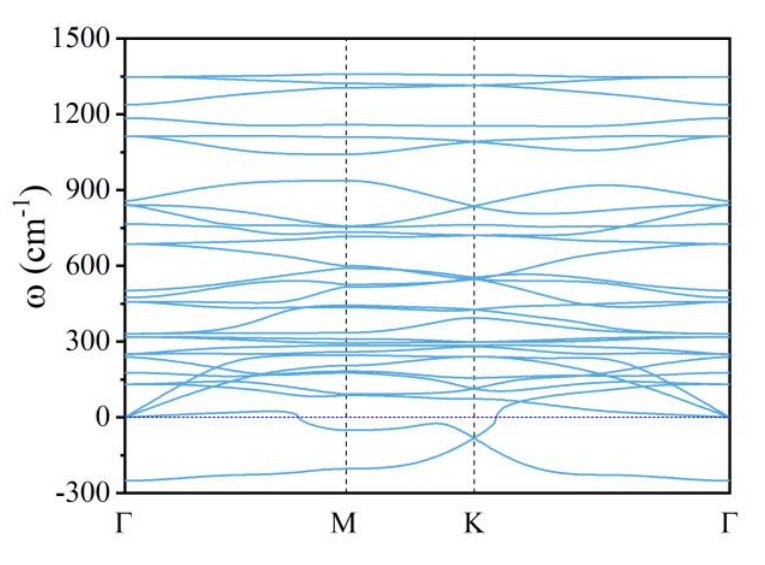
\includegraphics[width=0.72\textwidth]{figs/ch5_tib9_phonon_a.png}
  \centering
  \caption{全平的\ce{TiB9}的声子谱。}
  \label{fig:ch5_tib9_phonon_a}
\end{figure}

\subsection{双层TiB7的超导性质}
因为之前报道的有超导性质的过渡金属硼二维材料都是多层的构型,我们考虑通过将\ce{TiB7}堆积为双层构型是否能够提高其超导性质。如下图\ref{fig:ch5_stack_tib7},展示了\ce{TiB7}单层堆叠后形成的双层的声子谱及声子线宽$\gamma_{\bm{q}j}$,Eliashhberg函数$\alpha^2 F(\omega)$和$\lambda(\omega)$($\omega$。可以确定的是,从图?的AB形式堆叠的\ce{TiB7}双层的声子谱可以看出,声子谱中没有虚频说明结构可以在叠层状态稳定存在。
但相比于单层堆叠的\ce{TiB7}构型,双层的\ce{TiB7}费米能级处的电子密度$N(\epsilon_F)$下降了近25\%(如图\ref{fig:ch5_stack_tib7}),因此导致电声耦合系数$\lambda$下降了约22\%,超导转变温度下降了34\%。

从图中可以看出,在该双层构型中,同样是是低频(<400cm-1)的振动模式贡献了主要的电声耦合。根据McMillan–Allen–Dynes方程,我们可以估计超导临界温度$T_c$为5.5K。

\begin{figure}
  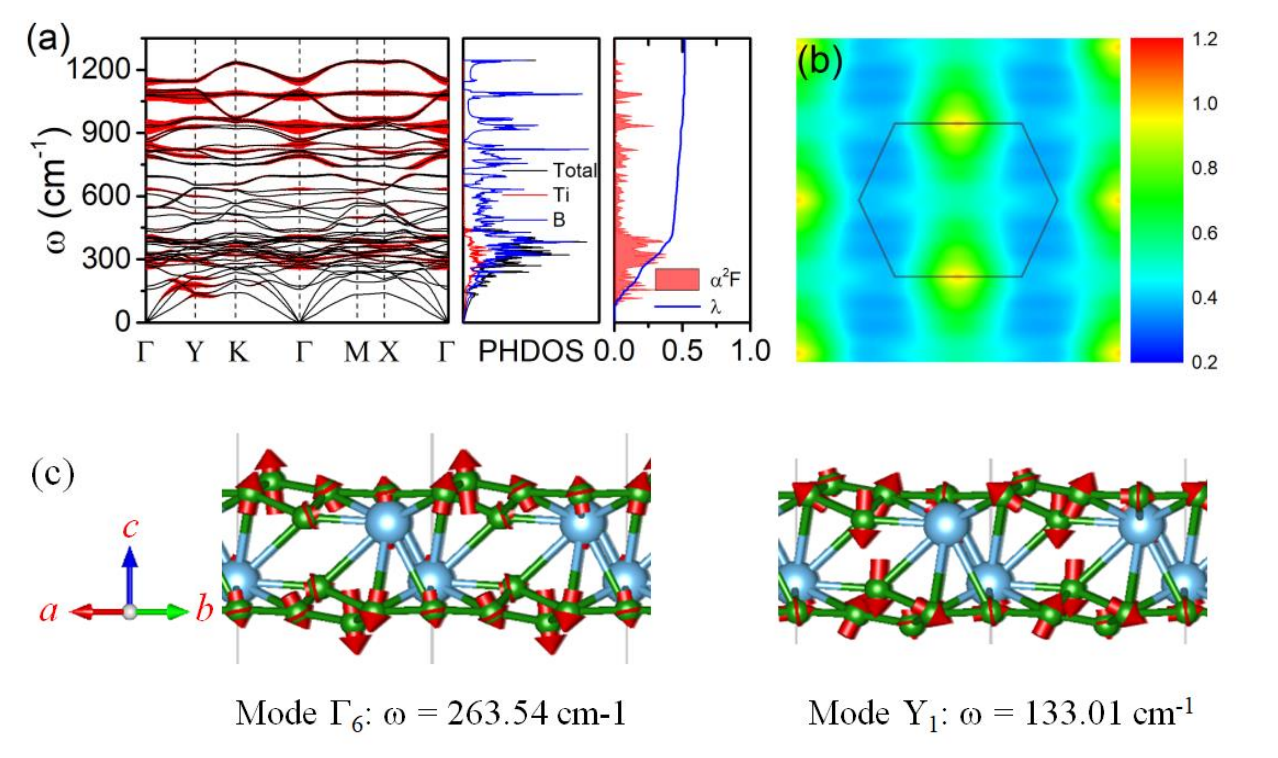
\includegraphics[width=0.96\textwidth]{figs/ch5_stack_tib7.png}
  \centering
  \caption{AB方式堆叠的\ce{TiB7}单层薄膜的声子色散以声子线宽$\gamma_{qj}$、声子态密度、Eliashberg函数$\alpha^2 F(\omega)$和$\lambda(\omega)$和耦合常数强度在倒空间的分布。}
  \label{fig:ch5_stack_tib7}
\end{figure}

与单层\ce{TiB7}超导性质计算时相同,经验公式中的库伦排斥势mu我们依然选取使用了$\mu=0.1$来计算超导转变温度。图\ref{fig:ch5_stack_tib7}中展示了电声耦合系数$\lambda_{\bm{q}}$在到空间中的变化情况,我们可以看到,声子线宽在$Y$对称点附近为最大,这是与单层\ce{TiB7}所不同的,且该处的电声耦合系数为最大值$\lambda_{\bm{q}}\approx 1$。从振动模式中可以看出,在堆叠后双层\ce{TiB7}中每个单层都不再是全平的平面结构,而有原子的起伏,这使得原先单层中对电声有较大贡献的面内的旋转振动模式不再出现。与单层\ce{TiB7}相同,双层\ce{TiB7}的电声耦合同样主要来源于原子质量较轻的硼原子。
我们将本文所研究的和已经报道的钛硼结构的电声耦合和超导性质总结在表\ref{table:sc_all}中。

\begin{table}
  \centering
  \begin{tabular}{lllll}
    \hline\hline
    compounds & $N(\epsilon_F)$ & $\omega_\mathrm{log}$ & $\lambda$ & $T_c$ \\
    \hline
    \ce{TiB7}单层 & 1.78 & 290.47 & 0.65 & 8.3 \\
    \ce{TiB7}双层 & 1.32 & 409.90 & 0.51 & 5.5 \\
    \ce{TiB9}单层 & 2.25 & 325.97 & 0.40 & 1.2 \\
    \ce{TiB4}单层 & 1.21 & 484.87 & 0.18 & 0.0 \\
    \ce{Ti2B2}单层 & 7.96 & 326.75 & 0.27 & 0.0 \\
    \hline
  \end{tabular}
  \caption{各种二维钛硼结构的超导性质}\label{table:sc_all}
\end{table}


%%%%%%%%%%%%%%%%%%%%%%%%%%%%%%%%%%%%%%%%%%%%%%%%%%%%%%%%%%%%%%%%%%%%%%%%%%%%%%%
% 学位论文的正文应以《结论》作为最后一章
\chapter{结论与展望}\label{chapter_concludes}

本文在第1章介绍了硼材料结构和性质上的多样性,引出了我们最后一张中的研究对象钛硼结构。

在第二章中介绍了在研究中使用到的计算材料能量和超导性质的第一性原理方法的详细细节。

从第三章开始,我们介绍并实现了周期结构的查重和生成算法。周期性体系从原胞出发能够拓展出各种各样的衍生结构,这些衍生结构中存在大量的物理等价的构型。
构型的总数随着超胞体积的扩大增加的非常迅速,我们通过使用厄米标准型矩阵来对表示衍生的晶格并作用晶格的对称操作后进行对比查重。针对固定的衍生晶格,我们对晶格位点进行了编号,后续的对称操作能够等价于对编号的置换操作。同时合并使用对不同的衍生的超晶格的HNF矩阵进一步划分归类,将具有相同的SNF矩阵的归为同类。同类超晶格可以有相同的商群,因而有相同的不等价的标号顺序。通过这个方法,我们能够快速的对一系列具有相同SNF矩阵的晶格排除平移操作。因此大大提高了查重效率。
我们从实践上通过自己编写的软件实现了对这类衍生结构的查询,并向用户提供了友好的命令行以及网页端的接口来完成查重任务。

再在第四章中介绍了本论文使用以及本人参与开发维护的高通量工具流工具AiiDA的架构设计。该章主要介绍了这一工具其内核架构上为了满足FAIR数据原则数据可重复性在数据可重用性上扮演了重要的作用,所采用的设计和实现。在高通量计算材料学的研究中使用该工具,能够大大减少科研人员在操作上的事件成本,并使得原来难以管理的海量数据得到很好的整合,方便在将来容易地对结果进行分析,以及将结果与同行分享。

最后讨论综合以上的方法和工具对钛硼单层结构基于特定结构上的特征,加入先验的结构上的限制,有偏地对各个配比的单层钛硼结构生成大量处在势能面局域极小值附近的初始构型。之后进行结构的优化和能量的评定,从而挑选出各个配比下能量较优的构型进行进一步的性质的探索。我们主要对\ce{TiB7}最稳定的构型进行了超导性质的计算,认为它有很好的超导性质。使用相同的方法,我们希望可以在未来的研究工作中将体系拓展到夹层结构以及多层结构,甚至相同的方法和流程能够适用于有特定结构特征的体相结构的生成户搜索。方法本身相比成熟的全局搜索算法在结构有特定结构特征时搜索的构型空间更小,从而大大节约了计算成本,并且由于该方法逻辑上简洁明了只需要一步来生成所有候选构型,使得能够容易地使用高通量工具流工具和后续的性质计算连接,以进行更多复杂的性质方面的分析和计算。

%%%%%%%%%%%%%%%%%%%%%%%%%%%%%%%%%%%%%%%%%%%%%%%%%%%%%%%%%%%%%%%%%%%%%%%%%%%%%%%
% 致谢,应放在《结论》之后
\begin{acknowledgement}
  首先感谢我的母亲韦春花对我的支持。其次感谢我的导师陈近南对我的精心指导和热心帮助。接下来,
  感谢我的师兄茅十八和风际中,他们阅读了我的论文草稿并提出了很有价值的修改建议。

  最后,感谢我亲爱的老婆们:双儿、苏荃、阿珂、沐剑屏、曾柔、建宁公主、方怡,感谢
  你们在生活上对我无微不至的关怀和照顾。我爱你们!
\end{acknowledgement}

%%%%%%%%%%%%%%%%%%%%%%%%%%%%%%%%%%%%%%%%%%%%%%%%%%%%%%%%%%%%%%%%%%%%%%%%%%%%%%%
% 附录
\appendix

\chapter{博士(硕士)学位论文编写格式规定(试行)}


\subsection{致谢}

可以在正文后对下列方面致谢:

\begin{itemize}
\item 国家科学基金、资助研究工作的奖学金基金、合作单位、资助或支持的企业、组织或个
人;
\item 协助完成研究工作和提供便利条件的组织或个人;
\item 在研究工作中提出建议和提供帮助的人;
\item 给予转载和引用权的资料、图片、文献、研究思想和设想的所有者;
\item 其他应感谢的组织或个人。
\end{itemize}

% 参考文献。应放在\backmatter之前。
% 推荐使用BibTeX,若不使用BibTeX时注释掉下面一句。
\nocite{*}
\bibliography{main}

% % 附录,必须放在参考文献后,backmatter前
% \appendix
% \chapter{图论基础知识}
% \Blindtext
%
% %%%%%%%%%%%%%%%%%%%%%%%%%%%%%%%%%%%%%%%%%%%%%%%%%%%%%%%%%%%%%%%%%%%%%%%%%%%%%%%
% % 书籍附件
% \backmatter
%%%%%%%%%%%%%%%%%%%%%%%%%%%%%%%%%%%%%%%%%%%%%%%%%%%%%%%%%%%%%%%%%%%%%%%%%%%%%%%
% % 作者简历与科研成果页,应放在backmatter之后
% \begin{resume}
% % 论文作者身份简介,一句话即可。
% \begin{authorinfo}
% \noindent 韦小宝,男,汉族,1985年11月出生,江苏省扬州人。
% \end{authorinfo}
% % 论文作者教育经历列表,按日期从近到远排列,不包括将要申请的学位。
% \begin{education}
% \item[2007年9月 --- 2010年6月] 南京大学计算机科学与技术系 \hfill 硕士
% \item[2003年9月 --- 2007年6月] 南京大学计算机科学与技术系 \hfill 本科
% \end{education}
% % 论文作者在攻读学位期间所发表的文章的列表,按发表日期从近到远排列。
% \begin{publications}
% \item Xiaobao Wei, Jinnan Chen, ``Voting-on-Grid Clustering for Secure
%   Localization in Wireless Sensor Networks,'' in \textsl{Proc. IEEE International
%     Conference on Communications (ICC) 2010}, May. 2010.
% \item Xiaobao Wei, Shiba Mao, Jinnan Chen, ``Protecting Source Location Privacy
%   in Wireless Sensor Networks with Data Aggregation,'' in \textsl{Proc. 6th
%     International Conference on Ubiquitous Intelligence and Computing (UIC)
%     2009}, Oct. 2009.
% \end{publications}
% % 论文作者在攻读学位期间参与的科研课题的列表,按照日期从近到远排列。
% \begin{projects}
% \item 国家自然科学基金面上项目``无线传感器网络在知识获取过程中的若干安全问题研究''
% (课题年限~2010年1月 --- 2012年12月),负责位置相关安全问题的研究。
% \item 江苏省知识创新工程重要方向项目下属课题``下一代移动通信安全机制研究''
% (课题年限~2010年1月 --- 2010年12月),负责LTE/SAE认证相关的安全问题研究。
% \end{projects}
% \end{resume}

%%%%%%%%%%%%%%%%%%%%%%%%%%%%%%%%%%%%%%%%%%%%%%%%%%%%%%%%%%%%%%%%%%%%%%%%%%%%%%%
% 生成《学位论文出版授权书》页面,应放在最后一页
% \makelicense

%%%%%%%%%%%%%%%%%%%%%%%%%%%%%%%%%%%%%%%%%%%%%%%%%%%%%%%%%%%%%%%%%%%%%%%%%%%%%%%
\end{document}
